% This template was originally by R. Jacob Vogelstein
% Updated on March 1, 2010 by Noah J. Cowan


\documentclass[12pt,oneside,final]{thesis}

\usepackage[superscript]{cite}
\usepackage{amsmath,amsfonts}
\usepackage{graphicx}
\graphicspath{{./figs/}}
\usepackage{fixltx2e}
\usepackage{array}
% wrapfig is fragile: use sparingly
\usepackage{wrapfig} 
%\usepackage{times}  % Use this for ugly fonts

\usepackage{upgreek}
\usepackage{hyperref}
\usepackage{setspace}

\usepackage{booktabs}
\usepackage{multirow}
\usepackage{longtable}
\usepackage[font=singlespacing, labelfont=bf]{caption}
%\usepackage{CV}

\usepackage{enumitem}
\newlist{inlinelist}{enumerate*}{1}
\setlist*[inlinelist,1]{%
  label=(\arabic*),
}

\usepackage{fancyhdr}    % Use nice looking headers along with the required footer page numbers   
%\usepackage[hypertex]{hyperref}

\DeclareMathOperator{\tr}{tr}

%Define the header/footer style
\pagestyle{fancy}
\fancyhf{}
\setlength{\headheight}{15pt}
\lhead{\leftmark}
\cfoot{\thepage}
\renewcommand{\headrulewidth}{0pt}
\fancypagestyle{plain}{% Redefine ``plain'' style for chapter boundaries
\fancyhf{} % clear all header and footer fields
\fancyfoot[C]{\thepage} % except the center
\renewcommand{\headrulewidth}{0pt}
\renewcommand{\footrulewidth}{0pt}}

%\tolerance=10000

%\makeglossary % enable the glossary

% Carl's packages
\usepackage{color}
\usepackage{import}
\usepackage{amssymb}
\usepackage{wasysym}
\usepackage{bm}
%\usepackage{mathrsfs} 

% Colors
\definecolor{forest_green}{RGB}{60,160,60}
\definecolor{co1}{rgb}{0, 0.4470, 0.7410}
\definecolor{co2}{rgb}{0.8500, 0.3250, 0.0980}
\definecolor{co3}{rgb}{0.9290, 0.6940, 0.1250}
\definecolor{co4}{rgb}{0.4940, 0.1840, 0.5560}
\definecolor{co5}{rgb}{0.4660, 0.6740, 0.1880}
\definecolor{co6}{rgb}{0.3010, 0.7450, 0.9330}
\definecolor{co7}{rgb}{0.6350, 0.0780, 0.1840}
\definecolor{gray}{rgb}{0.5, 0.5, 0.5}
\definecolor{MPLred}{RGB}{214, 39, 40}
\definecolor{MPLgreen}{RGB}{44, 160, 44}
\definecolor{MPLorange}{RGB}{255, 127, 14}
\definecolor{MPLblue}{RGB}{32, 119, 180}

% Line styles
\newcommand{\dashed}{\protect\mbox{-\; -\; -\; -}}
\newcommand{\full}{\protect\mbox{------}}
\newcommand{\broken}{\protect\mbox{-- -- --}}
\newcommand{\dashdot}{\protect\mbox{---\; -}}


% tikz for block diagrams
\usepackage{tikz}
\usetikzlibrary{shapes,arrows}
\usetikzlibrary{positioning}
\usetikzlibrary{calc}
\usetikzlibrary{automata}
\tikzstyle{block} = [draw, rectangle, minimum height=3.5em, minimum width=5em]
\tikzstyle{dblock} = [draw, dashed, rectangle, minimum height=3.5em, minimum width=5em]
\tikzstyle{io} = [coordinate]
\tikzstyle{pinstyle} = [pin edge={to-,thin,black}]

\begin{document}

% Title page
\title{Large-eddy simulations, wake models, and control: Power grid frequency support with wind farms}
\author{Carl Robert Shapiro}
\degreemonth{September}
\degreeyear{2018} 
\dissertation
\doctorphilosophy
\copyrightnotice

% currsize is not set in the long table environment, so we need to set it before we set it up.
\makeatletter
\let\@currsize\normalsize
\makeatother

% Chapters
%% FRONTMATTER
\begin{frontmatter}

% generate title
\maketitle

\begin{abstract}
Improved integration of wind farms into frequency regulation services is vital for increasing renewable energy production while maintaining power system stability. In particular, wind farms of the future will need to be able to provide secondary frequency regulation by tracking a power reference signal controlled by the grid operator. Wind farm wake models, estimation methods, and control techniques are developed to improve wind farm secondary frequency regulation capabilities. Large-eddy simulations (LES), where the large scales are directly simulated, are combined with the actuator disk model, which represents a wind turbine as a drag disk, to simulate large wind farms. LES provides an ideal test bed for wake model validation and control algorithm development. A dynamic wind farm model is developed for time-varying changes in wind farm thrust and validated against LES of a wind farm at start up. A new yawed wind turbine theory is derived for the near-disk inviscid region of the flow and compared to numerical simulations. This model yields more accurate predictions of the initial transverse velocity and wake skewness angle than existing models. We use these predictions as initial conditions in an extended dynamic wake model for yawed turbines and compare predicted wake deflection with wind tunnel experiments. Sensing and estimation methods are developed to assimilate power measurements into the new dynamic wake model. Using LES, the dynamic wake model, and sensing and estimation methods, we propose the use of model-based receding horizon control to provide secondary frequency regulation for a power grid using thrust coefficient modulation.  We implement the controller in high-fidelity numerical simulations of a wind farm with 84 turbines and then test the controlled farm's ability to track a power reference signal. The results demonstrate the ability of the control algorithm to track two types of power reference signals used by a US independent system operator. Furthermore, the controller achieves accurate power tracking and reduces loss of revenue in the bulk power market by requiring less setpoint reduction (derate) than the power level control range. The control design is subsequently extended to include generator torque, blade pitch actuation, and the rotational inertia of the rotor. 

\vspace{1cm}

\noindent Primary Readers and Advisors: Dennice Gayme and Charles Meneveau\\
Secondary Reader: Enrique Mallada

\end{abstract}

\begin{acknowledgment}

I am forever indebted to the numerous people who supported me throughout my doctoral studies. First and foremost, I am grateful for the support of my advisors, Professors Dennice Gayme and Charles Meneveau, for their patience, kindness, and encouragement. Thank you to Professor Johan Meyers, for both his technical guidance as well as his generosity and hospitality during my visits to KU Leuven. I must also thank Professor Enrique Mallada for serving on my dissertation and GBO committees, Professors Ben Hobbs and Sauleh Siddiqui for serving on my GBO committee, and the many wonderful professors who made my education possible. This dissertation was also made possible by the financial support of the National Science Foundation through grants ECCS 1230788, OISE 1243482, and CMMI 1635430, as well as the computational resources of the Maryland Advanced Research Computing Center (MARCC).

For the love and support of my parents, Donna and Martin, who taught me to care about what is right, I am eternally gratefully. To my sister, Anna, for her friendship, humor, and shared love of politics, food, and furry creatures. And of course, thank you to my partner, Zo\'{e}, whose love, intellect, and kindness never ceases to amaze me. To Quince for always being herself. To all of my friends and colleagues at Hopkins and KU Leuven --- Ismail, Tony, Juliaan, Joel, Dan, Michelle, Eshwan, Sean, Claire, Adrien, Perry, Ted, Vaughan, Richard, Michael, Di, Mike, Xiang, Wim, Thanos, Dries, Adam, Elina, Brent, Cindy, Robin, and Anna --- for their fun and enriching conversations. And to Baltimore for never ceasing to charm me along the way.

\end{acknowledgment}

\begin{dedication}
\topskip0pt
\vfil
{\it 
%One possibility is just to tag along with the fantasists in government and industry who would have us believe that we can pursue our ideals of affluence, comfort, mobility, and leisure indefinitely. This curious faith is predicated on the notion that we will soon develop unlimited new sources of energy: domestic oil fields, shale oil, gasified coal, nuclear power, solar energy, and so on. This is fantastical because 
\noindent [T]he basic cause of the energy crisis is not scarcity; it is moral ignorance and weakness of character.}~\cite{Berry1996a}
\begin{flushright}
--- Wendell Berry
\end{flushright}
\vfil
\end{dedication}

% generate table of contents
\tableofcontents

% generate list of tables
\listoftables

% generate list of figures
\listoffigures

\end{frontmatter}

\chapter{Introduction}
\label{chap:intro}
\chaptermark{Introduction}

Worldwide electricity generation from non-hydroelectric renewable energy sources --- solar, wind, biomass, ethanol, and geothermal --- has grown considerably over the past several decades, increasing from 30 TWh in 1980 to almost 1,692 TWh in 2015~\cite{EIA2018a}. During this period of growth (see Figure~\ref{fig:gen-hist}), wind energy has played a leading role, increasing from 0.1 TWh in 1986 to over 833 TWh in 2015~\cite{EIA2018a}. Wind's exponential growth has been widespread, reaching, as a percent of total electricity generation, 9.8\% in the European Union (EU), 4.7\% in the United States (US), 3.3\% in China, and 1.5\% in the rest of the world~\cite{EIA2018a}. 

\begin{figure}[h!]
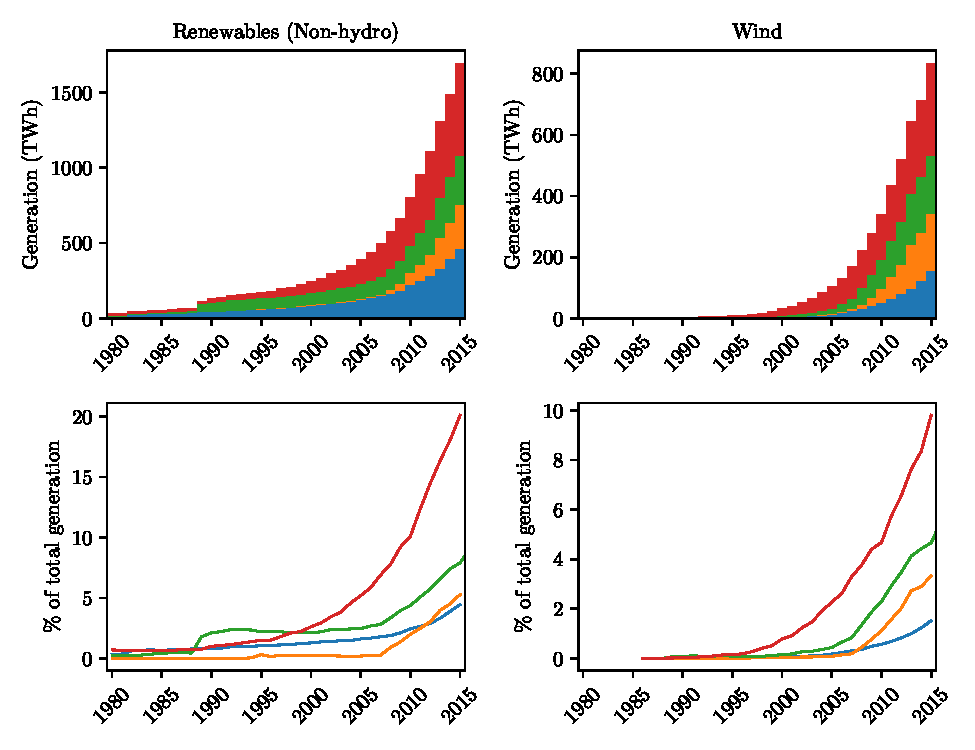
\includegraphics[width=\textwidth]{./wind-growth/gen-hist.pdf}
\caption{Growth in worldwide non-hydroelectric renewable electricity generation (left panels) and wind electricity generation (right panels). Renewable and wind generation are shown in TWh in the top panels and as a percentage of total generation in the bottom panels. Worldwide totals are displayed for the European Union ({\color{MPLred}\full}), United States ({\color{MPLgreen}\full}), China ({\color{MPLorange}\full}), and the rest of the world ({\color{MPLblue}\full}). Data from EIA~\cite{EIA2018a}.}
\label{fig:gen-hist}
\end{figure}

Wind's growth has not been uniformly distributed across the US and EU, with certain regions making significantly larger gains than other areas. In the EU, wind energy has reached nearly 50\% of total generation in Denmark, over 20\% in Ireland, Portugal, the Netherlands, and Lithuania, 18\% in Spain, and 13\% in Germany and the United Kingdom~\cite{EIA2018a}. In the US, wind generation is over 12\% of total generation in 11 states, including 31\% in Iowa and 25\% in South Dakota~\cite{GWEC2016a}.

The growth trends of wind have been driven by reduced costs and larger wind turbines. In the US, the levelized cost of energy for land-based wind has plummeted from nearly 600/MWh in 1980 to less than 50/MWh in 2015, and wind turbine rotor diameters and hub heights have increased from 17 m to over 100 m~\cite{DOE2015a}. As importantly, the environmental benefits of the move to wind energy are considerable. In the US, wind has reduced annual carbon dioxide emissions by 115,000,000 metric tons, sulfur dioxide emissions by 157,000 metric tons, nitrogen dioxide emissions by 97,000 metric tons, and water consumption by 36.5 billion gallons~\cite{DOE2015a}.

Wind energy's remarkable growth is expected to continue in the coming decades. The Global Wind Energy Center projects that wind will reach 15--40\% of global electricity demand by 2050, depending on future policy decisions~\cite{GWEC2016a}. In the US, the Department of Energy projects wind energy generation reaching 25\% of total demand by 2050 under 2015 policies with the potential to reach 35\% under more favorable policies~\cite{DOE2015a}.

\section{A challenge for grid integration of wind: Frequency regulation}
\label{sec:intro-freq-reg}
The continuing growth of variable and nondispatchable resources like wind energy has significant implications for the electric power system and will require changes in wind plant design and control. Over the last several years, wind has been operated as a niche energy source and grid operators have treated wind energy as a ``must take'' resource~\cite{Gil2013a}. As a result, wind plants prioritized maximizing power production because they were paid for every unit of power they produced. With growing grid penetration, however, wind energy has a growing potential to affect the overall state of the grid. A particular challenge for reliable power system operations under increased wind generation are ancillary services that maintain the stability of the grid~\cite{DOE2015a}. This has led grid operators and regulators to start requiring wind plants to participate in many of these services~\cite{Aho2012a, DiazGonzalez2014a}. 

Frequency regulation, which keeps the grid operating around its nominal frequency rating, is a particularly important ancillary service. Power systems currently rely on conventional dispatchable power sources to provide frequency regulation through short-term balancing of active power generation and load. As variable resources displace conventional generation, the resulting concern about the future availability of sufficient regulation participation has led many grid operators to consider expanding the pool of participating resources to include unconventional resources like wind energy~\cite{Aho2012a, DiazGonzalez2014a}. However, enabling full wind energy participation in frequency regulation involves many technological and economic challenges. A successful strategy will require new control designs that focus on power tracking rather than maximizing power output~\cite{Aho2012a}, modified frequency regulation market structures~\cite{Ela2014a, Ela2014b, Ela2014c}, expanded interconnection requirements for wind farms~\cite{Aho2012a, DiazGonzalez2014a}, and consideration of economic trade-offs between bulk power supply payments, ancillary service payments, and possible coordination with energy storage technologies~\cite{Rose2014a, Kirby2010a, DiazGonzalez2015a, Sun2010a}. 

Frequency regulation services act over many time scales to limit the deviation of the grid frequency from its nominal operating value in response to a grid disturbance, such as the failure of a major power plant of power transmission line. These services are classified into four categories of service, which each operate over a distinct time scale and serve a specific function. Figure~\ref{fig:freq-reg} shows the response of the grid frequency after a major generation loss and the time scales of each regulation service category.

\begin{figure}[h]
\begin{center}
\subimport{./fig/}{freq_reg.pdf_tex}
\end{center}
\caption{Response of power grid frequency to a major generation loss and the time scales of each regulation service category. Figure adapted from Aho \textit{et al.}~\cite{Aho2012a}.}
\label{fig:freq-reg}
\end{figure}

After a grid disturbance, inertial regulation acts instantaneously to limit the rate of frequency change and the maximum frequency deviation that occurs within several seconds. Primary regulation (droop control) acts over many seconds to drive the grid frequency towards a new steady-state operating value. Secondary regulation (automatic generator control) restores the system to its nominal frequency value by commanding participating generators to follow a power signal set by the grid operator over tens of minutes. Finally, tertiary regulation involves manually redistributing generation resources to restore normal operating conditions over several hours~\cite{Aho2012a, Rebours2007a, Rebours2007b}. 

Frequency regulation strategies using wind energy have focused on the first three regulation services because tertiary services occur over long time scales during which wind energy is too variable to provide balancing services. Instead, tertiary regulation is addressed through better scheduling, unit commitment, forecasting, or transmission system expansion~\cite{DOE2008a}. Combined inertial and primary regulation controls using wind turbines have been quite successful~\cite{Holdsworth2004a, Almeida2007a, Ma2010a, Morren2006a, Erlich2010a, Miller2011a, Hansen2014a}, even reducing the maximum and settling frequency deviation more effectively than traditional generators~\cite{Miller2011a, Gevorgian2015a}. Since aerodynamic interactions between turbines are relatively unimportant at time scales of less than a minute, combined inertial/primary controls can be implemented at the turbine level. 

With the success of inertial and primary frequency regulation control strategies, recent studies have begun to focus on secondary regulation~\cite{Buckspan2012a, Buckspan2013a, Aho2013a, Aho2014a, Jeong2014a, vanWingerden2017a, Boersma2017a}. Power plants participating in secondary frequency regulation typically provide power in both the bulk power market and the regulation market. The bulk power is supplied at some fixed level $P_0$ and the regulation service entails providing $\Delta P$ of regulation power that is controlled by the grid operator through the normalized regulation signal $r(t)$. The combined reference signal the plant must track is
\begin{equation}
P_\text{ref}(t) = P_0 + \Delta P \, r(t).
\end{equation}
Two example secondary regulation signals from PJM, a grid operator in the US that includes Baltimore, Maryland within its operating territory, are shown in Figure~\ref{fig:pjm}. As seen in these signals, the regulation signals vary on time scales on the order of minutes.

\begin{figure}[h]
\begin{center}
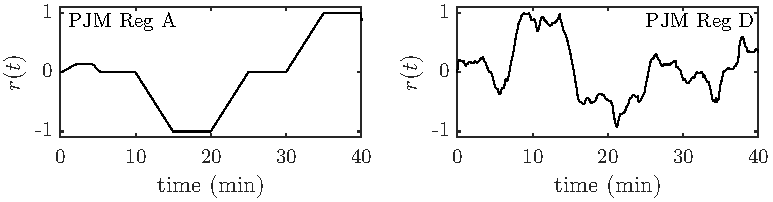
\includegraphics[width=\textwidth]{./fig/pjm.pdf}
\end{center}
\caption{Regulation signals from PJM~\cite{PJMm11, PJM2018a}, which has two regulation markets "RegA" and "RegD".}
\label{fig:pjm}
\end{figure}

A stand-alone turbine can regulate its instantaneous power output level through pitch and/or generator torque control, which enables it to follow a secondary regulation signal. While current wind turbine controllers operate at the maximum power point $P_*$, participation in the secondary frequency regulation market --- which includes increased power demand over the bulk power setpoint --- requires a wind turbine to reduce the amount of power it provides to the bulk power market~\cite{Aho2012a, Rose2014a, Kirby2010a, Aho2013a, Jeong2014a, Fleming2016a}. A particularly effective approach~\cite{Aho2013a} is to modify the generator torque control law such that the turbine operates at a higher-than-optimal tip speed ratio, thereby storing energy in the rotating rotor. Since a single wind turbine cannot provide power production greater than the maximum power point for an extended period, the derated generation setpoint is the maximum power point minus the regulation power; i.e. $P_0 = P_* - \Delta P$. This procedure is known as derating the turbine's power output. 

As a result, wind energy suppliers must consider the trade-offs between lost bulk power supply payments and additional ancillary service payments~\cite{Rose2014a, Kirby2010a}. Rose \& Apt~\cite{Rose2014a} found that these economic tradeoffs mean that given the current energy market design wind turbines can only provide secondary regulation more cost effectively that conventional generators less than 1\% of the time. This lack of profitability for providing regulation is because the secondary regulation price in competitive markets is equal to the lowest opportunity cost for a generator to provide regulation. This opportunity cost is the wholesale price of electricity less the generator's marginal cost that is dominated by fuel costs. A conventional generator's marginal cost is a significant fraction of the wholesale electricity price and a wind plant has a near zero marginal cost because wind is free~\cite{Rose2014a}. Therefore, wind energy is unlikely to have a lower opportunity cost than conventional generators. Kirby \textit{et al.}~\cite{Kirby2010a} found similar tradeoffs, but noted that in cases of high wind generation, conventional generators are forced to pay high costs related to minimum loads and regulation prices remain relatively stable. This makes wind energy cost competitive during some time periods~\cite{Kirby2010a}. Rose and Apt~\cite{Rose2014a} also note that the cost of developing secondary regulation controllers is low and should be required as an additional grid stability contingency. 

\section{Providing secondary frequency regulation with wind farms}
\label{sec:intro-secondary-wind}
In addition to the economic challenges outlined above, applying the single-turbine approach to wind farms is not straightforward because aerodynamic interactions between turbines complicate controlling the power output of an entire farm. Wind turbines in a farm are aerodynamically coupled by wakes, which are regions of reduced velocity and increased turbulence behind the turbines, depicted by the fog shown in Figure~\ref{fig:wind_farm_wake}. Control actions at an individual wind turbine modify the strength and characteristics of the wake behind the rotor, which in turn affects the subsequent power production of downstream turbines as the wake travels downwind and interacts with wakes of subsequent and adjacent turbines. In large wind farms, this complicated aerodynamic coupling is unavoidable. Wind turbine wakes extent tens of rotor diameters downstream, and moving downstream turbines away from the wakes of upstream turbines is impossible in practice given space constraints.

Several aerodynamic control variables can affect wind farm power output in a dynamic and coupled manner. Thrust modulation through pitch or generator torque control~\cite{Annoni2015b} affects the magnitude of the velocity behind the wake. Yawing, where the turbine is misaligned with the incoming wind direction, can redirect wakes toward or away from downstream turbines~\cite{Fleming2014a, Fleming2015a}. Tilting of the rotor can also dynamically affect wind farm power by redirecting wakes and modifying the entrainment of kinetic energy~\cite{Fleming2014a, Verhulst2015a, Annoni2017a}.

For example, suppose thrust modulation is employed at a turbine at the beginning of the farm. If the turbine pitches its blades from a feathered configuration toward the optimal pitch angle, the power generation at that turbine will increase and the velocity in the turbine's wake will be reduced. As a result, the generation of downstream turbines will decrease, but only after the wake has traveled to the downstream turbine. This complex and time-varying aerodynamic coupling of upstream turbine control actions and downstream turbine power generation is a particular challenge for secondary frequency regulation because the travel time of the wind from one turbine to the next and the time it takes the wind to travel the length of the farm is routinely the same or longer than the duration and frequency of typical regulation signals.

\begin{figure}[h]
\begin{center}
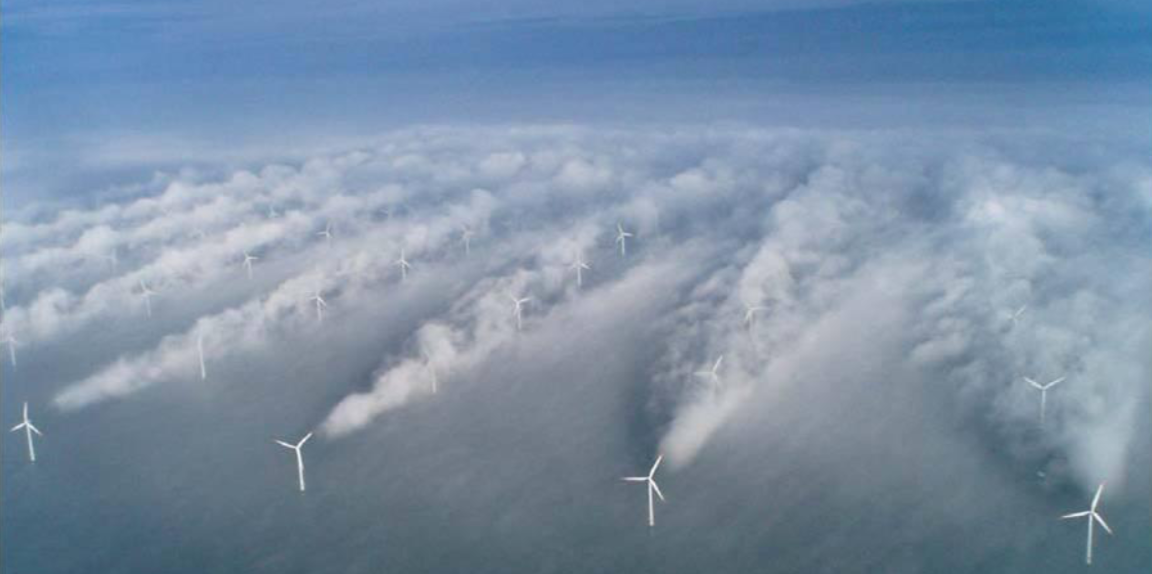
\includegraphics[width=\textwidth]{./fig/wind_farm.png}
\end{center}
\caption{Wind turbine wakes in Horns Rev wind farm visualized by the formation of fog. Figure is reproduced from Hasager \textit{et al.}~\cite{Hasager2013a} and licensed under CC BY 3.0.}
\label{fig:wind_farm_wake}
\end{figure}

Clearly, providing secondary regulation for the power grid with wind farms is more complicated than the single turbine case. Issues have been demonstrated in numerical simulations of a wind farm where each wind turbine employs a tracking method that neglects aerodynamic interactions~\cite{Fleming2016a}. When downstream turbines were placed away from upstream wakes, the farm was able to track the secondary frequency regulation signal. However, when downstream turbines were placed in the wakes of upstream turbines, the tracking performance of the downstream turbines was significantly degraded. 

One successful single-turbine approach was a proportional-integral controller that employs the same single-turbine control strategy but compensates for underperforming turbines by increasing the power production of other turbines operating below the maximum power point~\cite{vanWingerden2017a}. The resulting closed-loop wind farm provides good tracking performance in tests employing high-fidelity simulations as a wind farm model. However, the derate used~\cite{vanWingerden2017a} was larger than the regulation power, sacrificing considerable revenue in the bulk power market. As a result, approaches that do not consider interactions between turbine wakes~\cite{Hansen2006a, Hansen2006b} or use steady-state wake models that ignore the time-varying nature of these interactions~\cite{Ahmadyar2015a, Badihi2015a} may be unable to provide secondary frequency regulation. Ultimately, given the complexity of the aerodynamic interactions between turbines, more work is needed to develop effective controls for secondary frequency regulation. 

\section{Wind farm models and control}
\label{sec:intro-models}
Wind farm control designs have generally relied on model-based approaches to address the complexity of wind farm aerodynamics. Available wind farm models vary tremendously in complexity and accuracy. Static wake models have played a leading role in wind farm design for decades. The Jensen model~\cite{Jensen1983a, Katic1986a} treats the initial wake as a top-hat profile with an initial deficit specified using actuator disk theory~\cite{Burton2011a} and assumes that the diameter of the wake expands linearly with downstream distance through turbulent mixing, as shown in Figure~\ref{fig:jensen}. Other wake-centric models have mirrored this approach~\cite{Ainslie1988a, Bastankhah2014a, Niayifar2015a, Niayifar2016a, Archer2018a, Frandsen2006a, Gebraad2014c}. Top-down models~\cite{Frandsen1992a, Frandsen2006a, Calaf2010a, Meneveau2012a} view the wind farm as an added roughness that affects the entrainment of kinetic energy from above. Stevens~\textit{et al.}~\cite{Stevens2015a, Stevens2016c} recently coupled these two approaches to improve the results.

\begin{figure}[h]
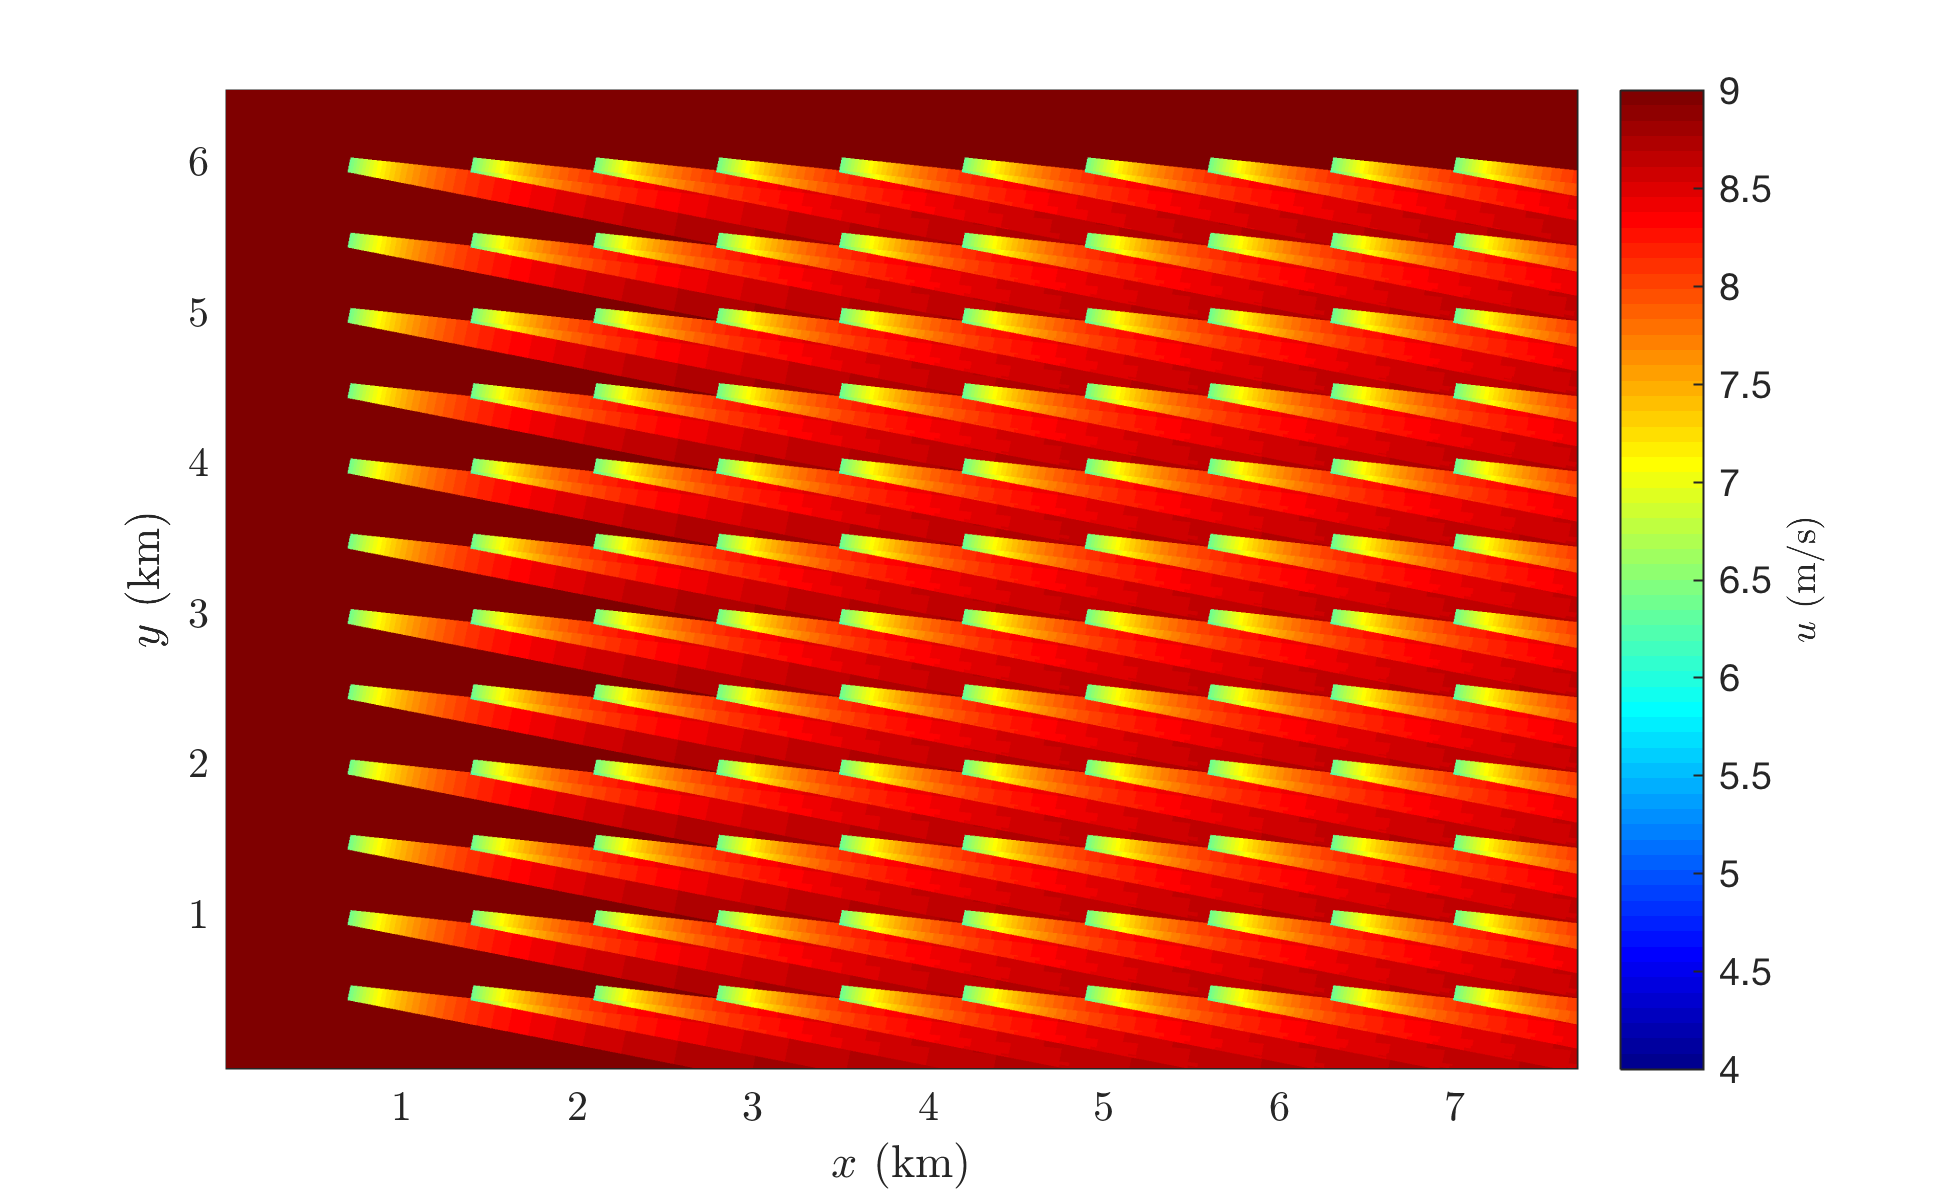
\includegraphics[width=\textwidth]{./fig/jensen.png}
\caption{Jensen model of a wind farm with 120 turbines with an inflow of $U_\infty = 9$ m/s.}
\label{fig:jensen}
\end{figure}

These static wake models, however, are unable to model yawed and tilted turbines. Wake models that account for these effects, unfortunately, have not been as successful in predicting wind farm behavior. Most notably, momentum balance arguments~\cite{Burton2011a, Jimenez2010a}, Glauert's proposed equation for the axial induced velocity through the rotor~\cite{Glauert1926a}, and the skewed elliptic vortex cylinder model~\cite{Coleman1945a, Branlard2016a} lead to conflicting results that do not always agree with simulations of yawed wind farms. Resolving the significant differences among these models is vital for providing secondary frequency regulation control with yawing or tilting.

Although static wake models have improved wind farm design and analysis, these models lack dynamics to model the effects of time-dependent changes in thrust coefficients and other operating conditions in general. In recent years, dynamic models have been proposed that account for the movement of wakes through the wind farm as well as turbulent mixing of wakes with the surrounding air through extensions of the classic Jensen wake model~\cite{Larsen2008a, Annoni2016b, Gebraad2014b, Gebraad2015b}. Higher-fidelity approaches include input-output dynamic mode decomposition~\cite{Annoni2016a}, the restricted nonlinear model~\cite{Bretheim2018a}, and the two-dimensional Navier-Stokes equations~\cite{Doekemeijer2017a, Boersma2018a}. Despite these advances, fully functioning wind farm controllers have yet to be built around these dynamic modeling approaches.

Control designs using high-fidelity simulations have been used successfully for similar problems, including drag reduction in turbulent boundary layers~\cite{Bewley2001a} and power maximization of wind farms~\cite{Goit2015a}. In these studies, numerical simulations of the flow states of these systems were taken as state-space representations, and control trajectories were determined by solving an online optimization problem using adjoint-based gradient methods. While this approach could also be applied to the secondary frequency regulation power tracking problem, the size of the optimization problem is too large to be solved in real time in any foreseeable future~\cite{Goit2015a}. 

\section{Outline}
\label{sec:intro-outline}
This thesis works towards a unified control framework for power tracking with wind farms using thrust and yaw modulation. Furthermore, we aim to reduce the derate requirements for wind farms providing secondary frequency regulation by storing energy in the wind flow field or the rotation of the rotor.  (See Appendix~\ref{app} for estimates of energy storage potential). This project includes (1) building dynamic wake models that account for the physics of wake advection, wake expansion through turbulent mixing, and wake deflection through yaw; (2) developing sensing and estimation tools to correct modeling errors using measurements from wind farms; and (3) developing controllers to provide power tracking with the error corrected models. The rest of this thesis is organized into the following chapters.

In Chapter~\ref{chap:methods}, we discuss the methods and tools used to develop and evaluate wind farm controls, including large eddy simulations and optimal control of PDE systems. In Chapter~\ref{chap:dynwake}, a dynamic wake model is presented that includes wake advection and expansion. A lifting line approach is used in Chapter~\ref{chap:yaw} to develop wake models that accurately predict the deflection of wakes behind yawed turbines. Sensing and estimation methods for the dynamic wake model are discussed in Chapter~\ref{chap:estimation}. Chapter~\ref{chap:rhc} presents the model-based receding horizon controller used to provide secondary frequency regulation and evaluates the control method using grid operator performance metrics and compares the control to a controller build around a static model. Chapter~\ref{chap:rhc2} discusses extensions of the controller presented in Chapter~\ref{chap:rhc} to allow for arbitrary wind farm configurations and incorporate rotor dynamics and inertia as well as realistic wind farm control variables. Conclusions and future work are discussed in Chapter~\ref{chap:conclusions}.
\chapter{Methods}
\label{chap:methods}
\chaptermark{methods}

In this thesis, high-fidelity large-eddy simulations and optimal control of systems governed by partial differential equations (PDE) are used extensively. Large-eddy simulations of wind farms,~\cite{Calaf2010a, Meyers2010a, Wu2011a, Wu2012a, Cater2012a, Churchfield2012a, Wu2013a, Stevens2014a, Stevens2014b, Stevens2014c, VerHulst2014a, Goit2015a, Wu2015a, Munters2016a, Munters2017a, Stevens2018a, Martinez2018a, Allaerts2018a} discussed in Section~\ref{sec:methods-les}, are used primarily as a means of evaluating the accuracy of wake models and serving as a ``virtual wind farm'' for testing control designs. In lieu of a physical installed wind farm to conduct control experiments or collect data, these simulation provide a cheap, yet accurate, way to rapidly develop models, sensing techniques, and control designs. In Section~\ref{sec:methods-pdeopt}, optimal control of PDE-constrained systems is discussed. This methodology will be used extensively to develop the secondary frequency regulation controllers of Chapters~\ref{chap:rhc} and~\ref{chap:rhc2}. 

\section{Large-eddy simulations of wind farms}
\label{sec:methods-les}

The neutrally-buoyant flow over a wind farm is governed by the incompressible Navier-Stokes equations
\begin{align}
\frac{\partial u_i}{\partial x_i} &= 0 \\
\frac{\partial u_i}{\partial t} + u_j \frac{\partial u_i}{\partial x_j} &= - \frac{1}{\rho} \frac{\partial p}{\partial x_i}   - \nu \frac{\partial^2 u_i}{\partial x_j \partial x_j} + f_i
\end{align}
where $u_i$ is the $i$-th component of the velocity, $\rho$ is the density of the air,  $\nu$ is the kinematic viscosity, $p$ is the pressure, and $f_i$ is the $i$-th component of the force per unit mass imposed by the turbine on the flow. Einstein's summation convention is used for repeated indices. Direct numerical simulation (DNS) of the Navier-Stokes equations over wind farms pose insurmountable hurdles due to scale disparity. The range of scales present in large wind farms ranges from the length of the farm itself, which can reach several kilometers long, to the Kolmogorov microscale~\cite{Tennekes1972a} $\eta = (\nu^3/\epsilon)^{1/4}$ or the viscous sublayer on the turbine blades. The dissipation rate $\epsilon \sim u_*^3/H$ is related to the friction velocity of $u_*$ and  atmospheric boundary layer height $H$. Assuming $u_*= 0.5$ m/s and a boundary layer height of $H = 1000$ m, the Kolmogorov microscale is approximately $\eta = 2$ mm. Near the blades, the scales become even smaller, on the order of the blade viscous layer height, $\nu/u_{*bl} = 0.01$ mm, where $u_{*bl}$ is on the order of 2 m/s. As a result, DNS of flow over wind farms will be impossible for the foreseeable future. 

Fortunately, large-eddy simulations provide a path forward that is both tractable and retains much of the accuracy of DNS. This allows LES to be used to develop simple analytic wind farm models and as a ``plant model" for testing wind farm control designs. Instead of directly solving all scales present in the flow, a filtering operation $\widetilde{\cdot}$ is applied to the Navier-Stokes equations that removes scales smaller than the filter width $\Delta$. Applying the filtering operations to the Navier-Stokes equations yields
\begin{align}
&\frac{\partial \tilde{u}_i}{\partial x_i} = 0 \\
&\frac{\partial \tilde{u}_i}{\partial t} + \frac{\partial}{\partial x_j} \widetilde{u_j u_i} = - \frac{1}{\rho}\frac{\partial \tilde{p}}{\partial x_i} + \nu \frac{\partial^2 \tilde{u}_i}{\partial x_j \partial x_j} + \tilde{f}_i,
\end{align}
While filtering does not have the same properties as averaging, i.e $\tilde{\tilde{f}} \ne \tilde{f}$, we can decompose the advective term in a similar way to the Reynolds stress $\overline{u'_ju'_i} = \overline{u_ju_i} - \bar{u}_j\bar{u}_i$
\begin{equation}
\widetilde{u_j u_i} = \tilde{u}_j \tilde{u}_i + \left(   \widetilde{u_j u_i} - \tilde{u}_j \tilde{u}_i \right) = \tilde{u}_j \tilde{u}_i  + \sigma_{ij},
\end{equation}
where $\sigma_{ij} = \widetilde{u_j u_i} - \tilde{u}_j \tilde{u}_i$ is the subgrid stress tensor. After applying this decomposition, the filtered equations become
\begin{align}
&\frac{\partial \tilde{u}_i}{\partial x_i} = 0 \\
&\frac{\partial \tilde{u}_i}{\partial t} +\tilde{u}_j \frac{\partial \tilde{u_i}}{\partial x_j}  =  - \frac{\partial \sigma_{ij}}{\partial x_j}  - \frac{1}{\rho}\frac{\partial \tilde{p}}{\partial x_i} + \nu \frac{\partial^2 \tilde{u}_i}{\partial x_j \partial x_j} + \tilde{f}_i.
\end{align}
The viscous term is negligible after the filtering because the gradient of the filtered velocity is now smooth. The advective term can be written in a rotational form by adding a ``Bernoulli" term $-\tilde{u}_j \frac{\partial \tilde{u_j}}{\partial x_i} = - \frac{\partial}{\partial x_i} \left(\frac{1}{2}\tilde{u}_j \tilde{u}_j \right)$. We can also decompose the subgrid stess tensor into a deviatoric part by removing its trace $\sigma_{ij} = \tau_{ij} + \frac{1}{3}\sigma_{kk} \delta_{ij}$. The trace of the subgrid stress and the Bernoulli term can then be subsumed into a modified pressure $\tilde{p}^* = \tilde{p}/\rho + \frac{1}{3}\sigma_{kk} + \frac{1}{2}\tilde{u}_j \tilde{u}_j $. These simplifications lead to the filtered Navier-Stokes equations
\begin{align}
&\frac{\partial \tilde{u}_i}{\partial x_i} = 0 \\
&\frac{\partial \tilde{u}_i}{\partial t} +\tilde{u}_j \left( \frac{\partial \tilde{u_i}}{\partial x_j}  - \frac{\partial \tilde{u_j}}{\partial x_i} \right)=  - \frac{\partial \tau_{ij}}{\partial x_j}  - \frac{\partial \tilde{p}^*}{\partial x_i} + \tilde{f}_i.
\end{align}

\subsection{Flow solver}
\label{subsec:methods-les-solver}
In this thesis, the filtered Navier-Stokes equations are solved using the large-eddy simulation code LESGO~\cite{LESGO}. LESGO, which descends from the LES code of Albertson~\cite{Albertson1999a}, has been used to simulate air pollutant transport in urban canopies~\cite{Tseng2006a}, flow over fractal trees~\cite{Graham2012a}, buoyant plumes from oil well blowouts~\cite{Yang2016a}, heat entrainment under arctic sea ice~\cite{Ramudu2017a}, and flow over wind turbines~\cite{Martinez2018a} and wind farms~\cite{Calaf2010a, Stevens2014b, Verhulst2015a, Stevens2018a}. Written in rotational form, LESGO ensures mass, momentum, and kinetic energy conservation~\cite{Albertson1999a}. LESGO simulates Cartesian domains using psuedo-spectral numerics that mixes spectral derivatives in the streamwise direction $x$ and spanwise direction $y$ with second-order finite-differencing in the vertical direction $z$. Time integration uses the second-order Adams-Bashforth method. The advective term is calculated in spectral space and dealiased using the 3/2-rule~\cite{Orszag1975a}. The pressure is found from the pressure Poisson equation, which is solved using the tridiagonal matrix algorithm in the vertical direction and spectrally in the horizontal directions. The (nonlinear) right hand side of the Poisson equation is evaluated pseudo-spectrally. LESGO can be run in parallel using the message passing interface, where the domain is split between processors in the vertical direction.

The code uses a staggered grid in the vertical direction, where the $u$ and $v$ components of velocity and the pressure $p$ are stored on the $uv$ grid and the $w$ component of velocity is stored on the $w$ grid. Vertical derivatives or evaluated on the opposing grids, e.g. $\frac{\partial u}{\partial z}$ is evaluated on the $w$ grid. The first grid point of the $w$ grid starts at $z=0$, and the first grid point of the $uv$ grid is at $z=\Delta z/2$, where $\Delta z$ is the vertical grid size.

The stress at a wall with a roughness height of $z_0$ is modeled using the equilibrium wall model~\cite{Albertson1999a}. The total wall stress is given by
\begin{equation}
\tau_w = - \left[  \frac{\kappa u_\tau}{\ln(z/z_0)} \right]^2,
\end{equation}
where $z = \Delta z/2$ is the height from the wall, $\kappa$ is the von-K\'{a}rm\'{a}n constant, and $u_\tau$ is the velocity magnitude 
\begin{equation}
u_\tau^2 = \tilde{u}^2 + \tilde{v}^2
\end{equation}
at $z$. The wall stress is then apportioned to each component~\cite{Schmidt1989a} as
\begin{equation}
\left.\tau_{i3}\right\vert_{\text{wall}}= \tau_w \frac{\tilde{u}_i}{u_\tau}.
\end{equation}
At the wall, a no-penetration conditions is applied for $w$. At horizontal boundaries without walls, a stress-free boundary condition is applied, where the vertical derivatives of the $u$ and $v$ components of the velocity vanish, and a no-penetration condition is applied for $w$.

We consider domains with prescribed inflow conditions. LESGO's standard configuration uses a periodic boundary condition for the inflow, which naturally arises from the pseudo-spectral numerics. In this configuration, a wall is usually applied at the bottom boundary and the flow is driven using a streamwise pressure gradient. The resulting force term is 
\begin{equation}
\tilde{f}_i = -\frac{1}{\rho}\frac{\partial p_\infty}{\partial x} \delta_{i1} + \tilde{f}^a_i,
\end{equation}
where $p_\infty$ is the freestream pressure and $\tilde{f}^a_i$ are any other applied forces, such as forces representing the momentum losses due to wind turbines.

In cases with a prescribed inflow, the streamwise pressure gradient is not imposed. Instead, the inflow is imposed using a fringe region at the end of the domain. This fringe region smoothly transitions to a prescribed inflow velocity~\cite{Stevens2014a}. For uniform (laminar) inflow, the velocity field is transitioned to a constant $\tilde{u}_i(0,y,z) = U_\infty \delta_{i1}$. For cases where an inflow for a developed boundary layer is needed, such as for a developing boundary layer or over a finite-sized wind farm, the inflow condition is sampled from a concurrently running simulation with periodic boundary conditions~\cite{Stevens2014a}.

\subsection{Subgrid stress models}
\label{subsec:methods-les-subgrid}
In order to solve the filtered Navier-Stokes equations, a closure is needed for the subgrid stress tensor $\tau_{ij}$. The eddy viscosity model uses an analogy with ordinary viscosity
\begin{equation}
\tau_{ij} = - 2 \nu_T \tilde{S}_{ij}
\end{equation}
where $\tilde{S}_{ij}$ is the filtered strain rate tensor
\begin{equation}
 \tilde{S}_{ij} = \frac{1}{2}\left( \frac{\partial \tilde{u}_i}{\partial x_j} + \frac{\partial \tilde{u}_j}{\partial x_i}\right).
\end{equation}
(Note that the viscous term can be written as $\frac{\partial}{\partial x_j} 2 \nu S_{ij} = \frac{\partial}{\partial x_j} \nu \left(\frac{\partial u_i}{\partial x_j} + \frac{\partial u_i}{\partial x_j} \right) = \nu \frac{\partial^2 u_i}{\partial x_j \partial x_j}$ because of incompressibility and constancy of $\nu$.) The difficulty with the eddy viscosity model is to write a suitable model for the eddy viscosity $\nu_T$. In this thesis, we will use two subgrid stress closures, the Smagorinsky model and the Lagrangian-averaged scale-dependent (LASD) model.

\subsubsection{Smagorinsky model}
\label{subsubsec:methods-les-subgrid-smag}
The Smagorinsky subgrid stress model~\cite{Smagorinsky1963a} uses the strain rate tensor again for a velocity scale, which dimensionally requires another length scale. Since the subgrid stress only represents scales smaller than the filter size $\Delta$, this is the only suitable selection of this length scale. The resulting Smagorinsky model is 
\begin{equation}
\nu_T = C_s^2 \Delta^2 \vert \tilde{S} \vert \qquad \qquad \vert \tilde{S} \vert^2 = 2 \tilde{S}_{ij} \tilde{S}_{ij}
\end{equation}
where $C_s$ is the Smogorinsky coefficient. In the inertial subrange of high-Reynolds-number turbulence, Lilly showed that the appropriate Smagorinsky coefficient for a spectral cutoff filter is $C_s \approx 0.16$~\cite{Lilly1966b, Pope2000a}.

For wall bounded flows, the value $C_s = 0.16$ is overly dissipative towards the wall. Instead, the Mason wall damping model~\cite{Mason1994a} is used to specify the Smagorinsky coefficient. In this model, the mixing length $\lambda = C_s \Delta$ depends on the height from the wall
\begin{equation}
\lambda^{-n} = \lambda_0^{-n} + \left[\kappa (z + z_0)\right]^{-n},
\end{equation}
where $n =2$, $\kappa$ is the von-K\'{a}rm\'{a}n constant, $z$ is the height from the wall, $z_0$ is the surface roughness height, and $\lambda_0 = C_0 \Delta$ is the mixing length with the Lilly-Smagorinsky coefficient $C_0 = 0.16$.

\subsubsection{Lagrangian-averaged scale-dependent model}
\label{subsubsec:methods-les-subgrid-lasd}
The basic idea behind dynamic subgrid stress models is to use multiple filter sizes to measure the Smagorinsky coefficient in the resolved scales of the flow~\cite{Germano1992a, Bou-Zeid2005a}. Let $\tilde{\cdot}$ denote a filtering operation of a scale $\Delta$ and $\bar{\cdot}$ denote a test filter on scale $\alpha \Delta$, where $\alpha > 1$. We define the test-filtered filtered Navier-Stokes equations as
\begin{equation}
\frac{\partial \bar{\tilde{u}}_i}{\partial t} + \frac{\partial}{\partial x_j} \bar{\tilde{u}}_j\bar{\tilde{u}}_i  = - \frac{\partial T_{ij} }{\partial x_j} - \frac{\partial \bar{\tilde{p}}^*}{\partial x_i},
\end{equation}
where $T_{ij}$ is the stress at scales bar-tilde. The Germano identity~\cite{Germano1992a} relates the stress at different scales $T$ and $\tau$ and results in the resolved stress tensor
\begin{equation}
L_{ij} = T_{ij} - \bar{\tau}_{ij} = - \bar{\tilde{u}}_j\bar{\tilde{u}}_i + \overline{\tilde{u}_j\tilde{u}}_i,
\end{equation}
which can be measured in the resolved part of the flow. Using the Smagorinsky model for both $T_{ij}$ and $\bar{\tau}_{ij}$
\begin{equation}
T_{ij} = 2C_{s,\alpha\Delta}^2 \left( \alpha \Delta\right)^2 \vert \bar{\tilde{S}} \vert \bar{\tilde{S}}_{ij} \qquad \qquad \bar{\tau}_{ij} = 2C_{s,\Delta}^2 \Delta^2 \overline{\vert \tilde{S} \vert \tilde{S}_{ij}},
\end{equation}
we can now define the tensor $M_{ij}$ based on the modeled values for $T_{ij}$ and $\bar{\tau}_{ij}$
\begin{equation}
C_{s,\Delta}^2 M_{ij} = T_{ij} - \bar{\tau}_{ij} =2 C_{s,\Delta}^2 \Delta^2 \left( \overline{\vert \tilde{S} \vert \tilde{S}_{ij}} - \alpha^2 \beta \vert \bar{\tilde{S}} \vert \bar{\tilde{S}}_{ij} \right),
\end{equation}
where $\beta = C_{s,\alpha\Delta}^2 / C_{s,\Delta}^2$. The error between the measurements and model is therefore
\begin{equation}
e_{ij} = L_{ij} -  C_{s,\Delta}^2 M_{ij}.
\end{equation}

The simplest approach is to assume scale invariance ($\beta = 1$) and minimize the averaged least-square error $\left \langle e_{ij} e_{ij} \right \rangle$.
\begin{equation}
\underset{C_{s,\Delta}}{\mathrm{min}} \qquad \qquad \left \langle e_{ij} e_{ij} \right \rangle = \left \langle L_{ij} L_{ij} \right \rangle - 2 C_{s,\Delta}^2 \left \langle L_{ij} M_{ij} \right \rangle + C_{s,\Delta}^4\left \langle M_{ij} M_{ij} \right \rangle,
\end{equation} 
where the averaging can be any suitable averaging operation. The squared error is minimized by finding the root of the derivative
\begin{equation}
\frac{d}{d C_{s,\Delta}} \left \langle e_{ij} e_{ij} \right \rangle = -4 C_{s,\Delta} \left \langle L_{ij} M_{ij} \right \rangle + 4C_{s,\Delta}^3\left \langle M_{ij} M_{ij} \right \rangle = 0,
\end{equation}
which yields the following equation for the Smagorinsky coefficient
\begin{equation}
 C_{s,\Delta}^2 = \frac{\left \langle L_{ij} M_{ij} \right \rangle}{\left \langle M_{ij} M_{ij} \right \rangle}.
\end{equation}

This scale-invariant approach can be applied using planar averaging or Lagrangian averaging along fluid paths~\cite{Bou-Zeid2005a}. Scale-dependent models can also be derived by using two test filters to determine the coefficient $\beta$~\cite{Porte-Agel2000a}. In this thesis, we use the most advanced form of the dynamic models, the Lagrangian-average scale-dependent (LASD) model, which performs averaging along fluid paths and includes scale dependence~\cite{Bou-Zeid2005a}.

\subsection{Wind turbine model}
\label{subsec:methods-les-turbine}
In a wind farm with $N$ turbines without additional applied forces, the filtered force that enters the filtered Navier Stokes equations is
\begin{equation}
\tilde{\boldsymbol{f}^a} = \sum_{n=1}^N \mathbf{f}_n(\mathbf{x},t),
\end{equation}
where $ \mathbf{f}_n(\mathbf{x},t)$ is the force per unit volume applied by the $n$-th turbine. LESGO includes the actuator line model~\cite{Martinez2018a}, which models the effects of individual blades, and the actuator disk model~\cite{Calaf2010a}, which only models the wind turbine as a drag disk. While the actuator line model is a better parameterization of detailed flow phenomena near the turbine blades and in the near wake, both models accurately predict far wake characterizations and power production~\cite{Stevens2018a}. Furthermore, for large wind farms with coarse grid resolution, the actuator line cannot be properly resolved. As a result, we use the actuator disk model, without rotation or tangential forces, that distributes the force across several grid points that together represent the turbine. 

The actuator disk model represents the wind turbine as a drag disk that exerts a uniform thrust force across its area. The actuator disk model applies directly to the inviscid flow past a drag disk with a uniform velocity $U_\infty$~\cite{Glauert1935a, Glauert1947a, Burton2011a}. The resulting thrust force magnitude of a turbine (dropping the indices that denote the turbine number) is
\begin{equation}
F = - \frac{1}{2} \frac{\pi D^2}{4} \rho C_T U_\infty^2,
\end{equation}
where $\rho$ is the fluid density, $C_T$ is the thrust coefficient, and $D$ is the diameter of the actuator disk. Applying mass conservation, momentum conservation, and Bernoulli's equation, the velocity at the disk $u_d$ and velocity deficit in the ultimate wake $\delta u_0$ 
\begin{equation}
u_d = U_\infty(1-a) \qquad \qquad \delta u_0 = 2 U_\infty a
\end{equation}
are found to depend on the induction factor $a$. This induction factor depends only on the thrust coefficient 
\begin{equation}
C_T= 4a(1-a).
\end{equation}
Since the power generated by the turbine is
\begin{equation}
P = -F u_d = \frac{1}{2} \frac{\pi D^2}{4} \rho C_P U_\infty^3,
\end{equation}
the power coefficient only depends on the induction factor
\begin{equation}
C_P= 4a(1-a)^2.
\end{equation}

This model can also be applied to the turbulent flow past a wind turbine. However, the inflow velocity $U_\infty$ becomes somewhat difficult to define in wind farms. The solution is a local approach~\cite{Meyers2010a, Calaf2010a}, which writes the thrust force and power as
\begin{align}
F &= -\frac{1}{2} \frac{\pi D^2}{4} \rho C_T' u_d^2\\
P &= \frac{1}{2} \frac{\pi D^2}{4} \rho C_P' u_d^3,
\end{align}
where $C_T'$ is the local thrust coefficient and $C_P'$ is the local power coefficient. Using the results from the actuator disk theory, the relationships between the local and standard thrust and power coefficients are
\begin{equation}
C_T' = \frac{C_T}{(1-a)^2} \qquad \qquad C_P' = \frac{C_p}{(1-a)^3}.
\end{equation}
After some algebra, we find that
\begin{equation}
a = \frac{C_T'}{4 + C_T'} \qquad \qquad C_P' = C_T'.
\end{equation}

LESGO represents each wind turbine as an actuator disk with finite thickness $s$, which can be represented by the normalized indicator function, with units of inverse volume
\begin{equation}
\mathcal{I}(\mathbf{x}) = V^{-1}\left[ H(\hat{x}+s/2) - H(\hat{x} - s/2) \right] H(D/2 - \hat{r}),
\end{equation}
where $V = s \pi D^2/4$ is the volume of the disk, $H(x)$ is the Heaviside function, and $\hat{r}^2 = \hat{y}^2 + \hat{z}^2$. The coordinate system of the actuator disk is denoted by hats with the $\mathbf{\hat{e}_1}$ unit vector opposite of the thrust force. Since LESGO is a psuedo-spectral code, using the normalized indicator function to apply the thrust force on the flow directly would create Gibbs phenomena around the actuator disk. Instead, LESGO uses a smoothed indicator function
%
\begin{equation}
\mathcal{R}(\mathbf{x}) = \int G(\mathbf{x}-\mathbf{x'}) \, \mathcal{I}(\mathbf{x'}) \, d^3\mathbf{x'}
\end{equation}
%
based on a three-dimensional Gaussian kernel. The kernel
%
\begin{equation}
\label{eq:LESGO-Gaussian-kernel}
G(\mathbf{x}) = \left(\frac{6}{\pi \Delta^2}\right)^{3/2} \exp \left( -\frac{6\lVert\mathbf{x}\rVert^2}{\Delta^2} \right)
\end{equation}
%
has a filter width $\Delta = 1.5 h $ that is based on the grid size $h = \sqrt{\Delta x^2 + \Delta y^2 + \Delta z^2}$, where $\Delta x$, $\Delta y$, and $\Delta z$ are the grid spacings.  

The smoothed indicator function can be decomposed 
\begin{equation} \mathcal{R}(\mathbf{x}) = \mathcal{R}_1(\hat{x}) \mathcal{R}_2(\hat{r})
\end{equation}
into a normal component 
\begin{equation}
\mathcal{R}_1(\hat{x}) = \frac{1}{s} \left(\frac{6}{\pi \Delta^2}\right)^{1/2} \int \left[ H\left(\hat{x}'+\frac{s}{2}\right) - H\left(\hat{x}' - \frac{s}{2}\right) \right] \exp \left( -6\frac{(\hat{x}-\hat{x}')^2}{\Delta^2} \right) \, d \hat{x}' 
\end{equation} and radial component
 \begin{equation} 
 \mathcal{R}_2(\hat{r}) = \frac{1}{A}\frac{6}{\pi \Delta^2} \int \int H(D/2 - \hat{r}') \exp \left( -6\frac{(\hat{y}-\hat{y}')^2 + (\hat{z}-\hat{z}')^2}{\Delta^2} \right) \, d \hat{y}' \, d \hat{z}',
\end{equation} 
where $A = \pi D^2/4$ is the swept area of the turbine and $s$ is the thickness of the actuator disk. LESGO calculates the the smoothed indicator function at each point using the analytic solution to the normal component
\begin{equation}
\mathcal{R}_1(\hat{x}) = \frac{1}{s}\frac{1}{2}\mathrm{erf}\left(\frac{\sqrt{6}}{\Delta}\left(x+\frac{s}{2}\right) \right) - \frac{1}{2}\mathrm{erf}\left(\frac{\sqrt{6}}{\Delta}\left(x-\frac{s}{2}\right) \right)
\end{equation}
and numerically computing $\mathcal{R}_2(\hat{r})$ on a grid finer than the simulation grid.

LESGO uses this local formulation and distributes the turbine thrust force using a smoothed normalized indicator function $\mathcal{R}(\mathbf{x})$ with time-filtering of the disk-averaged velocity 
\begin{equation}
\mathbf{f}(\mathbf{x}) = -\frac{1}{2} \frac{\pi D^2}{4} \rho C_T' \left\langle u_d\right\rangle_T^2 \mathcal{R}(\mathbf{x}) \,\mathbf{\hat{e}_1}.
\end{equation}
The disk averaged velocity is also found using the smoothed indicator function
\begin{equation}
u_d = \int \mathcal{R}(\mathbf{x}) \, \tilde{\mathbf{u}}(\mathbf{x}) \, d^3\mathbf{x},
\end{equation}
and time averaging is performed using an exponential filter with time scale $\tau$
\begin{equation}
\tau \frac{ d \left\langle u_d \right\rangle_T}{dt} = u_d - \left\langle u_d \right\rangle_T.
\end{equation}



\subsection{Finite wind farm simulation}
\label{subsec:methods-les-farm}
\begin{figure}[b!]
\begin{center}
\includegraphics[width=\textwidth]{./fig/les.eps}
\end{center}
\caption{\label{fig:les} Instantaneous streamwise velocity contours for a large eddy simulation with actuator disk turbine models, which are indicated by black dashes. Each turbine has a rotor diameter of $D = 100$ m and hub height of 100 m. The mean and maximum inlet velocities are approximately 9 m/s and 12 m/s, respectively. The inlet conditions are generated using a concurrent precursor simulation~\cite{Stevens2014a} shown at the beginning of the plotted domain.}
\end{figure}

In much of this thesis, we will consider a wind farm composed of 84 turbines arranged in $N=7$ rows of $M=12$ aligned columns. Each turbine has a 100 m rotor diameter $D$ and a 100 m hub height. The spacing between turbines is $7D$ in the streamwise direction and $5D$ in the spanwise direction. We assume a  local thrust coefficient of $C_T'= 1.33$ is representative of wind turbines operating in region 2~\cite{Calaf2010a, Stevens2014c}. Inlet conditions for the wind farm are generated using the concurrent-precursor method~\cite{Stevens2014a}. Both the farm and precursor domains have 9~km streamwise, 6~km spanwise, and 1~km vertical lengths. The number of grid points in each domain are $384 \times 256 \times 192$, i.e. a grid size of $\Delta x = \Delta y = 23.44$ m is used in the streamwise and spanwise spectral directions and a grid size of $\Delta z = 5.21$ is used in the finite-difference vertical direction. The forcing fringe region of the farm domain is 1.125~km long and the first row of turbines is located 1.4 km from the beginning of the domain. The LASD subgrid scale model is used. A color contour plot of a snapshot of the streamwise velocity is shown in Figure~\ref{fig:les}. Unless noted otherwise, the simulations in the remainder of this thesis use this wind farm and computational set up.


\section{Optimal control of PDE-constrained systems}
\label{sec:methods-pdeopt}
Optimization of systems governed by partial differential equations is important in a range of engineering applications. First developed in the work of Lions~\cite{Lions1971a}, PDE-constrained optimal control has been applied in the last few decades to a many fluid dynamics applications, such as drag reduction of turbulent boundary layers ~\cite{Bewley2001a} and power maximization of wind farms in the atmospheric boundary layer~\cite{Goit2015a}. In this thesis, we will largely follow the approaches of Borz\`{i} \& Schulz~\cite{Borzi2011a} and Goit \& Meyers~\cite{Goit2015a}. We will consider problems of the form
\begin{align}
\label{eq:pde_constrained1}
\underset{\mathbf{q}, \mathbf{u}}{\textrm{min}} &\qquad \mathcal{J}(\mathbf{q},\mathbf{u}) \\
\label{eq:pde_constrained2}
\text{subject to} &\qquad \mathbf{B}(\mathbf{q}, \mathbf{u}) = \mathbf{0},
\end{align}
where $\mathbf{q} \in Q$ are the states of the system, $\mathbf{u} \in U$ are the control variables, $\mathcal{J}:Q\times U \rightarrow \mathbb{R}$ is the cost functional, and $\mathbf{B}:Q \times U \rightarrow Z$ are the state equations (the constraining PDEs). We will assume that $Q$, $U$, and $Z$ are Hilbert spaces whose respective scalar products are denoted by $\langle \cdot, \cdot \rangle_Q$, $\langle \cdot, \cdot \rangle_U$, and $\langle \cdot, \cdot \rangle_Z$.

In practice, it is typically easier to solve an unconstrained problem, and we want a method that minimizes possible evaluations of the constraining PDEs. The formal Lagrangian approach described below allows the constrained problem to be reformulated as the minimization of an unconstrained functional whose value and gradients can be found using a single evaluation of a set of PDEs. This approach requires forming a Lagrangian functional, defining a suitable directional derivative and gradient, and specifying the optimality conditions in terms of PDE evaluations.

The PDE-constrained problem is reformulated as an unconstrained problem by incorporating the constraints into an augmented cost functional known as the Lagrangian. The Lagrangian $\mathcal{L}$ is the sum of the constrained cost functional and the scalar product of the the adjoint variables (Lagrange multipliers) $\mathbf{z} \in Z$ with the constraints $\mathbf{B}(\mathbf{q}, \mathbf{u})$
\begin{equation}
\mathcal{L}(\mathbf{q}, \mathbf{u}, \mathbf{z}) = \mathcal{J}(\mathbf{q}, \mathbf{u} ) + \left \langle \mathbf{z}, \mathbf{B}(\mathbf{q}, \mathbf{u}) \right \rangle_Z.
\end{equation}
The scalar product is defined here with respect to the Hilbert space of the adjoint variable and constraints $Z$.

In order to specify the first-order Karush-Kuhn-Tucker (KKT) optimality conditions~\cite{Boyd2004a}, we must first define a suitable generational of the directional derivative for scalar functionals on Hilbert spaces. The G\^{a}teaux derivative of $\mathcal{F}: X \rightarrow \mathbb{R}$, a functional defined on a Hilbert space $X$, in the direction $\boldsymbol \delta \mathbf{x} \in X$ is defined as
\begin{equation}
\mathcal{F}_\mathbf{x}(\boldsymbol \delta \mathbf{x}) = \left. \frac{d}{d\alpha} \mathcal{F}(\mathbf{x} + \alpha \boldsymbol \delta \mathbf{x}) \right\vert_{\alpha=0}.
\end{equation}
Using the Reisz representation theorem, we find that the directional derivative can be written as the scalar product of the gradient of $\mathcal{F}$ with respect to $\mathbf{x}$ and the direction $\boldsymbol \delta \mathbf{x}$
\begin{equation}
\mathcal{F}_\mathbf{x}(\boldsymbol \delta \mathbf{x}) = \left \langle \frac{\partial \mathcal{F}}{\partial \mathbf{x}}, \boldsymbol \delta \mathbf{x} \right \rangle_X.
\end{equation}


With this definition of the G\^{a}teaux derivative, the the KKT conditions are written as 
\begin{equation}
\mathcal{L}_\mathbf{z}(\boldsymbol \delta \mathbf{z}) = 0 \qquad \qquad \mathcal{L}_\mathbf{q}(\boldsymbol \delta \mathbf{q}) = 0 \qquad \qquad \mathcal{L}_\mathbf{u}(\boldsymbol \delta \mathbf{u}) = 0.
\end{equation}
By evaluating the G\^{a}teaux derivatives and rewriting in terms of a scalar product using the Reisz representation theorem, we can then identify the gradient of the Lagrangian. The G\^{a}teaux derivative of the Lagrangian with respect to the Lagrange multipliers yields
\begin{equation}
\mathcal{L}_\mathbf{z}(\boldsymbol \delta \mathbf{z}) = \left \langle \boldsymbol \delta \mathbf{z}, \mathbf{B}(\mathbf{q}, \mathbf{u})\right \rangle_Z = 0.
\end{equation}
Since the direction vector can be any arbitrary vector, we require that the second term in the scalar product vanishes. This simply returns the state equations $\mathbf{B}(\mathbf{q}, \mathbf{u}) = \mathbf{0}$.

When evaluating the G\^{a}teaux derivatives with respect to the state variables and input variables, we will encounter some linear operators that result from linearizing the state equations about $\left(\mathbf{q}, \mathbf{u}\right)$ in the direction $\left(\boldsymbol \delta \mathbf{q}, \boldsymbol \delta  \mathbf{u}\right)$
\begin{equation}
\frac{\partial \mathbf{B}}{\partial \mathbf{q}} \boldsymbol \delta \mathbf{q} + \frac{\partial \mathbf{B}}{\partial \mathbf{u}} \boldsymbol \delta \mathbf{u} = \mathbf{0},
\end{equation}
where $\frac{\partial \mathbf{B}}{\partial \mathbf{q}} : Q \rightarrow Z$ and  $\frac{\partial \mathbf{B}}{\partial \mathbf{u}} : U \rightarrow Z$ are linear operators that map the state and input vectors, respectively, to the Hilbert space containing the solution to $ \mathbf{B}(\mathbf{q}, \mathbf{u}) = \mathbf{0}$. The adjoints of these linear operators, $\left(\frac{\partial \mathbf{B}}{\partial \mathbf{q}} \right)^* : Z \rightarrow Q$ and $\left(\frac{\partial \mathbf{B}}{\partial \mathbf{u}} \right)^* : Z \rightarrow U$, map back to the state and input Hilbert spaces, respectively, and are defined by
\begin{align}
\left \langle \mathbf{z}, \frac{\partial \mathbf{B}}{\partial \mathbf{q}} \boldsymbol \delta \mathbf{q} \right \rangle_Z&=
\left \langle\left(\frac{\partial \mathbf{B}}{\partial \mathbf{q}} \right)^*  \mathbf{z}, \boldsymbol \delta \mathbf{q} \right \rangle_Q \\
\left \langle \mathbf{z}, \frac{\partial \mathbf{B}}{\partial \mathbf{u}} \boldsymbol \delta \mathbf{u} \right \rangle_Z&=
\left \langle\left(\frac{\partial \mathbf{B}}{\partial \mathbf{u}} \right)^*  \mathbf{z}, \boldsymbol \delta \mathbf{u} \right \rangle_U.
\end{align}
In these cases, the scalar products on each side of the equality are taken over different Hilbert spaces. This is a direct consequence of the Reisz representation theorem and the domain and range of the linear operators and their adjoints. The gradients of the cost functional are formally defined using the G\^{a}teaux derivative and the Reisz representation theorem. For example, the gradient $\frac{\partial \mathcal{J}}{\partial \mathbf{u}}$ is defined by writing the G\^{a}teaux derivative in its Reisz representation form
\begin{equation}
\mathcal{J}_\mathbf{u}(\boldsymbol \delta \mathbf{u}) = \left. \frac{d}{d\alpha} \mathcal{J}(\mathbf{u} + \alpha \boldsymbol \delta \mathbf{u}) \right\vert_{\alpha=0} = \left \langle \frac{\partial \mathcal{J}}{\partial \mathbf{u}}, \boldsymbol \delta \mathbf{u} \right \rangle_U.
\end{equation}

The G\^{a}teaux derivative of the Lagrangian with respect to the state variables, combined with the KKT conditions, yields
\begin{align}
\mathcal{L}_\mathbf{q}(\boldsymbol \delta \mathbf{q}) &= \left \langle \frac{\partial \mathcal{J}}{\partial \mathbf{q}}, \boldsymbol \delta \mathbf{q} \right \rangle_Q +  \left \langle \mathbf{z},  \frac{\partial \mathbf{B}}{\partial \mathbf{q}} \boldsymbol \delta \mathbf{q} \right \rangle_Z \\
&= \left \langle \frac{\partial \mathcal{J}}{\partial \mathbf{q}}, \boldsymbol \delta \mathbf{q} \right \rangle_Q +  \left \langle \left(  \frac{\partial \mathbf{B}}{\partial \mathbf{q}}\right)^*\mathbf{z},  \boldsymbol \delta \mathbf{q} \right \rangle_Q \\
&= \left \langle \frac{\partial \mathcal{J}}{\partial \mathbf{q}} + \left(  \frac{\partial \mathbf{B}}{\partial \mathbf{q}}\right)^*\mathbf{z},  \boldsymbol \delta \mathbf{q} \right \rangle_Q = 0.
\end{align}
Again noting that the direction $\boldsymbol \delta \mathbf{q}$ is arbitrary, we require the first term in the scalar product to vanish. This yields the adjoint equations
\begin{equation}
\label{eq:adjoint_eq}
\frac{\partial \mathcal{J}}{\partial \mathbf{q}} + \left(  \frac{\partial \mathbf{B}}{\partial \mathbf{q}}\right)^*\mathbf{z} = \mathbf{0}.
\end{equation}
Finally, the G\^{a}teaux derivative of the Lagrangian with respect to the input variables, combined with the KKT conditions, yields
\begin{align}
\mathcal{L}_\mathbf{u}(\boldsymbol \delta \mathbf{u}) &= \left \langle \frac{\partial \mathcal{J}}{\partial \mathbf{u}}, \boldsymbol \delta \mathbf{u} \right \rangle_U +  \left \langle \mathbf{z},  \frac{\partial \mathbf{B}}{\partial \mathbf{u}} \boldsymbol \delta \mathbf{u} \right \rangle_Z \\
&= \left \langle \frac{\partial \mathcal{J}}{\partial \mathbf{u}}, \boldsymbol \delta \mathbf{u} \right \rangle_U +  \left \langle \left(  \frac{\partial \mathbf{B}}{\partial \mathbf{u}}\right)^*\mathbf{z},  \boldsymbol \delta \mathbf{u} \right \rangle_U \\
&= \left \langle \frac{\partial \mathcal{J}}{\partial \mathbf{u}} + \left(  \frac{\partial \mathbf{B}}{\partial \mathbf{u}}\right)^*\mathbf{z},  \boldsymbol \delta \mathbf{u} \right \rangle_U.
\end{align}
Requiring the scalar product to vanish yields the design equations
\begin{equation}
\label{eq:design_eq}
\frac{\partial \mathcal{J}}{\partial \mathbf{u}} + \left(  \frac{\partial \mathbf{B}}{\partial \mathbf{u}}\right)^*\mathbf{z} = \mathbf{0}.
\end{equation}

Using the Lagrangian approach described above, the original problem can be solved by writing the constrained problem~\eqref{eq:pde_constrained1}--\eqref{eq:pde_constrained2} as a minimization of an unconstrained cost functional in two ways. First, the method of Lagrange multipliers results in the problem
\begin{align}
\underset{\mathbf{q}, \mathbf{u}, \mathbf{z}}{\textrm{min}} &\qquad \mathcal{L}(\mathbf{q},\mathbf{u}, \mathbf{z}),
\end{align}
whose gradient is given by
\begin{equation}
\nabla \mathcal{L} = \left(\mathbf{B}(\mathbf{q}, \mathbf{u}), \frac{\partial \mathcal{J}}{\partial \mathbf{q}} + \left(  \frac{\partial \mathbf{B}}{\partial \mathbf{q}}\right)^*\mathbf{z},  \frac{\partial \mathcal{J}}{\partial \mathbf{u}} + \left(  \frac{\partial \mathbf{B}}{\partial \mathbf{u}}\right)^*\mathbf{z} \right).
\end{equation}. 
Alternatively, the problem can be solved using the reduced cost functional
\begin{align}
\underset{\mathbf{u}}{\textrm{min}} &\qquad \tilde{\mathcal{J}}(\mathbf{u}),
\end{align}
where $\tilde{\mathcal{J}}(\mathbf{u}) = \mathcal{J}(\mathbf{q}(\mathbf{u}))$ is the reduced cost functional with $\mathbf{q}(\mathbf{u})$ denoting the solution to $\mathbf{B}(\mathbf{q}, \mathbf{u})  = \mathbf{0}$. With this approach, the state and adjoint equations are explicitly enforced by solving $\mathbf{B}(\mathbf{q}, \mathbf{u})  = \mathbf{0}$ and $\frac{\partial \mathcal{J}}{\partial \mathbf{q}} + \left(  \frac{\partial \mathbf{B}}{\partial \mathbf{q}}\right)^*\mathbf{z} = \mathbf{0}$, as discussed in the derivation of~\eqref{eq:adjoint_eq}. The design equation then gives the gradient of the reduced cost functional
\begin{equation}
\frac{\partial \tilde{\mathcal{J}}}{\partial \mathbf{u}} = \frac{\partial \mathcal{J}}{\partial \mathbf{u}} + \left(  \frac{\partial \mathbf{B}}{\partial \mathbf{u}}\right)^*\mathbf{z}.
\end{equation}

\subsection{Example}
\label{sec:methods-pdeopt-example}
In this section we consider an example of a PDE-constrained optimization problem that is solved using the reduced cost functional approach. Consider the PDE-constrained minimization problem
\begin{align}
\label{eq:example1}
\underset{q,u}{\textrm{min}} &\qquad \mathcal{J}(q,u) = \frac{1}{2}\int_\Omega \left( q(\mathbf{x}) - f(\mathbf{x})\right)^2 \, d\mathbf{x} + \frac{\gamma}{2} \int_\Omega u^2(\mathbf{x}) \, d\mathbf{x} \\
\label{eq:example2}
\text{subject to} &\qquad \nabla^2 q = -u(x)& \qquad & \hspace{-15em} \text{on} \quad \Omega\\
\label{eq:example3}
&\qquad q(\mathbf{x}) = 0 & \qquad & \hspace{-15em} \text{on} \quad \partial \Omega.
\end{align}
We will define the scalar product as 
\begin{equation}
\left \langle v, w \right \rangle = \int_\Omega v(\mathbf{x}) w(\mathbf{x}) \, d \mathbf{x}
\end{equation}
and the Lagrangian using
\begin{equation}
\mathcal{L}(q, u, z) = \mathcal{J}(q,u) + \int_\Omega z(\mathbf{x}) \left[ \nabla^2 q + u(\mathbf{x}) \right] \, d\mathbf{x}.
\end{equation}
The adjoint equations are found via
\begin{align}
\mathcal{L}_q(\delta q) &= \int_\Omega \left( q(\mathbf{x}) - f(\mathbf{x})\right) \delta q(\mathbf{x}) \, d\mathbf{x} +\int_\Omega z(\mathbf{x}) \nabla^2 \delta q \, d\mathbf{x} \nonumber \\
&= \int_\Omega \left( q(\mathbf{x}) - f(\mathbf{x})\right) \delta q(\mathbf{x}) \, d\mathbf{x} +\int_\Omega \nabla^2 z \delta q \, d\mathbf{x} - \int_\Omega  \delta q(\mathbf{x}) \nabla^2 z \, d\mathbf{x} \\
&= \int_\Omega \left[ q(\mathbf{x}) - f(\mathbf{x})- \nabla^2 z\right] \delta q(\mathbf{x}) \, d\mathbf{x} +\int_{\partial \Omega} \left( \nabla z \delta q\right) \cdot \mathbf{n} \, dS \nonumber \\
&= \int_\Omega \left[ q(\mathbf{x}) - f(\mathbf{x})- \nabla^2 z\right] \delta q(\mathbf{x}) \, d\mathbf{x} +\int_{\partial \Omega} \delta q(\mathbf{x}) \nabla z  \cdot \mathbf{n} \, dS +\int_{\partial \Omega} z(\mathbf{x}) \nabla \delta q  \cdot \mathbf{n} \, dS. \nonumber
\end{align}
Since $q$ vanishes on the boundary, the second term also vanishes. As a result, the adjoint equations become
\begin{align}
\label{eq:example_adjoint1}
&\nabla^2 z = q(\mathbf{x}) - f(\mathbf{x}) & \qquad & \text{on} \quad \Omega \\
\label{eq:example_adjoint2}
&z(\mathbf{x}) = 0 & \qquad & \text{on} \quad \partial \Omega.
\end{align}
The design equation is found using
\begin{equation}
\mathcal{L}_u(\delta u) = \gamma \int_\Omega u(\mathbf{x}) \delta u(\mathbf{x}) \, d\mathbf{x} + \int_\Omega z(\mathbf{x}) \delta u(\mathbf{x}) \, d\mathbf{x},
\end{equation}
which gives the gradient of the reduced cost functional as 
\begin{equation}
\label{eq:example_gradient}
\frac{\partial \tilde{\mathcal{J}}}{\partial u} = u(\mathbf{x}) + z(\mathbf{x}).
\end{equation}
The adjoint equations~\eqref{eq:example_adjoint1}--\eqref{eq:example_adjoint2} and gradient of the reduced cost function~\eqref{eq:example_gradient} allow us to solve the original constrained problem~\eqref{eq:example1}--\eqref{eq:example3} using a gradient-based optimization method.
\chapter{A simple dynamic wake model}
\label{chap:dynwake}
\chaptermark{A simple dynamic wake model}

Wind turbines extract momentum and energy from the wind, generating a wake that travels downstream. These wakes reduce the energy extraction and power production of downstream turbines; however, they also expand through turbulent mixing, thus partially recovering the energy available for subsequent turbines. To provide secondary frequency regulation, wind turbines can be used to modulate energy extraction, changing the properties of the wake generated at the turbine. For instance, if the energy extraction at one turbine is momentarily reduced, increased kinetic energy becomes available in its wake. However, this additional energy only becomes available to the downstream turbine after the flow travel time between these turbines has elapsed. In order to capture such effects quantitatively, we develop a dynamic wake model, drawing on the classic steady-state Jensen wake model~\cite{Katic1986a}, to include the time-varying impact of changing turbine kinetic energy extraction on total wind farm power production.

\section{The dynamics of a wind turbine wake}
\label{sec:dynwake-wakemodel}
We begin by considering the wake behind a single wind turbine. The coordinate system is defined such that the mean inflow velocity $U_\infty$ is directed in the positive $x$ direction, $y$ and $z$ denote the transverse directions, and the origin of the coordinate system is at the center of the rotor swept area. Considering the behavior of the wake in a Reynolds-averaged sense, i.e. solving for the ensemble mean velocity from the unsteady RANS equations, the wake behind a the turbine is governed by the Reynold-averaged mean momentum equation
\begin{equation}
\rho \frac{\partial u_i}{\partial t} + \rho u_j \frac{\partial u_i}{\partial x_j} = - \frac{\partial p}{\partial x_i} - \frac{\partial \tau_{ij}}{\partial x_j} + f_i,
\end{equation}
where $\rho$ is the density of air, $u_i(\mathbf{x},t)$ is the Reynolds-averaged velocity (for convenience we omit the ensemble averaging symbols), $p(\mathbf{x},t)$ is the mean pressure, $f_i(\mathbf{x},t)$ is the turbine thrust force per unit mass, and $\tau_{ij}$ the Reynolds stress tensor.  After neglecting the viscous terms, linearizing the advective term with the average inflow velocity $U_\infty$, i.e. $u_j \frac{\partial }{\partial x_j} = U_\infty \frac{\partial}{\partial x}$, and rewriting in terms of the local velocity deficit $U_\infty\delta_{i1} - u_i({\bf x},t)$, the Reynolds averaged mean momentum equation becomes
%
\begin{equation}
\label{eq:linearized_momentum_deficit}
 \rho \frac{\partial}{\partial t} (U_\infty\delta_{i1} - u_i) +  \rho U_\infty \frac{\partial }{\partial x}  (U_\infty\delta_{i1} - u_i) = \frac{\partial p}{\partial x_i} - f_i + \frac{\partial \tau_{ij}}{\partial x_j},
\end{equation}
As the wake travels downstream, the area of the wake will increase through turbulent mixing. If the expansion rate is determined only by the turbulence properties of the incoming flow, then the effective area of the wake $A(x)$ can be assumed to be a function of only the streamwise distance $x$ from the turbine. As a result, this wake area is constant in time and we implicitly neglect possible dependencies of wake expansion on temporal variations in the thrust coefficient.  Assuming that this effective area --- which will be specified shortly --- is known, the mean velocity deficit $\delta u_i(x,t)$ is defined as
\begin{equation}
\label{eq:area_velocity}
\delta u_i(x,t) = \frac{1}{A(x)}\int_{-\infty}^{\infty} \int_{-\infty}^{\infty}( U_\infty\delta_{i1} - u_i(x,y,z,t)) \, dy \, dz.
\end{equation}
Integrating~\eqref{eq:linearized_momentum_deficit} in the transverse directions, $y$ and $z$, yields
\begin{equation}
\label{eq:averaged_momentum}
\frac{\partial}{\partial t} \left[ \rho A(x) \delta u_i(x,t) \right] + U_\infty \frac{\partial }{\partial x} \left[ \rho  A(x) \delta u_i(x,t)\right] = \frac{\partial \bar{p}}{\partial x}\delta _{i1} - \bar{f}_i ,
\end{equation}
where $\bar{p}(x,t)$ and $\bar{f}_i(x,t)$ denote the transversely averaged pressure and thrust force and $\delta(x)$ is the Dirac delta function. Although the divergence of the Reynolds stress does not enter, the effects of turbulence are encoded in the modeled behavior of $A(x)$. 

Since the thrust force is confined to the rotor disk and the pressure gradient vanishes away from the turbine~\cite{Glauert1935a}, the right hand size of~\eqref{eq:averaged_momentum} only has to be considered in the region near the turbine rotor. The net effect of the pressure gradient and thrust force is therefore modeled as a source of momentum deficit
\begin{equation}
\frac{\partial \bar{p}}{\partial x}\,\delta _{i1} - \bar{f}_i = \rho A(x) \,S_i(t) \, \delta(x),
\end{equation}
where $S_i(t)$ may be time dependent in cases of varying turbine thrust. Substituting  into~\eqref{eq:averaged_momentum}, expanding the spatial derivatives, and dividing by $\rho A(x)$ yields
\begin{equation}
\label{eq:preliminary_deficit}
\frac{\partial \delta u_i}{\partial t} + U_\infty \frac{\partial \delta u_i }{\partial x} = - w(x) \,\delta u_i(x,t) + \,S_i(t) \, \delta(x),
\end{equation}
where the wake expansion rate is
\begin{equation}
w(x) = U_\infty  \frac{1}{A(x)} \frac{d A}{d x}.
\end{equation}

The source strength $S_i(t)$ is specified in a manner consistent with inviscid models of the initial velocity deficit behind the turbine.  In other words, the source strength is determined in such a way that the initial velocity deficit (just after a fluid parcel has passed through the turbine) is $\delta u_i(x=\epsilon) = \delta u_{0i} $, where $\delta u_{0i}$ is the initial velocity deficit known separately as predicted from an inviscid model and $\epsilon$ is a small displacement. To impose this initial velocity deficit, we integrate~\eqref{eq:preliminary_deficit} in $x$ between $x=-\epsilon$, where $\delta u_i(- \epsilon)=0$, and $x=\epsilon$. In this region, the rate of change of $A$ is negligible compared to the effects of the Dirac delta forcing. Hence,~\eqref{eq:preliminary_deficit} becomes $U_\infty  \frac{\partial \delta u_i}{\partial x} = S_i  \delta(x)$, and after integrating we obtain  $\delta u_i(\epsilon)=S_i / U_{\infty}$. Therefore, the source term is specified as $S_i = U_\infty \delta u_{0i}$.

In the unyawed case, the appropriate inviscid model is the actuator disk theory, discussed in Section~\ref{subsec:methods-les-turbine}, which gives an initial velocity deficit $\delta u_{i0} = 2 U_\infty a = 2 U_\infty C_T'/(4+C_T')$ that depends on the induction factor $a$ or the local thrust coefficient $C_T'$. As a result, the only velocity component that remains is in the streamwise direction, and the source term is $S_i(t) = 2 U_\infty a(t) \delta_{i1} = 2 U_\infty C_T'/(4+C_T') \delta_{i1}$. This procedure will properly specify the source of velocity deficit in the unyawed case, but in yawed or tilted cases a different inviscid model is needed, as will be discussed in Chapter~\ref{chap:yaw}.

Since we assume that the wake area is invariant in time, we can consider a steady flow to derive the correct expression for the wake area function
\begin{equation}
A(x)= \frac{\pi D^2}{4} d_w^2(x),
\end{equation}
which is written in terms of $d_w(x)$, the effective diameter of the wake normalized by turbine diameter $D=2R$. After linearizing the advective term, assuming the pressure gradient vanishes in the region sufficiently downstream from the turbine, neglecting the streamwise Reynolds stress, and using the eddy viscosity model, the Reynolds-averaged mean momentum equation for the streamwise velocity $u$ in the region away form the turbine forcing becomes
\begin{equation}
\label{eq:RANS_eddy_viscosity}
U_\infty \frac{\partial u}{\partial x} = \frac{1}{r} \frac{\partial}{\partial r} \left( r \nu_T  \frac{\partial u}{\partial r} \right),
\end{equation}
where $r$ is the distance from the center of the wake and $\nu_T$ is the eddy viscosity. Past research has noted that the far wake of a turbine has a self-similar profile~\cite{Bastankhah2014a}; therefore, the velocity may be written as
\begin{equation}
\label{eq:deficit_profile}
u(x,r) = U_\infty - \delta u(x) W\left(\frac{r}{\ell(x)}\right),
\end{equation}
where $W(\xi)$ is a self-similar function of $\xi = \frac{r}{\ell(x)}$ and $\ell(x) \sim D d_w(x)$ is proportional to the diameter of the wake. 

For a free wake, the eddy viscosity scales with the wake width and the velocity deficit $\nu_T \sim \delta u \, \ell$~\cite{Tennekes1972a}. In the atmospheric boundary layer, however, the appropriate velocity scale is the friction velocity $u_*$, giving the following eddy viscosity
\begin{equation}
\label{eq:eddy_viscosity}
\nu_T(x) = u_* \ell(x).
\end{equation}
Replacing~\eqref{eq:deficit_profile} and~\eqref{eq:eddy_viscosity} into~\eqref{eq:RANS_eddy_viscosity} and expanding the derivatives we obtain
\begin{equation}
-U_\infty \frac{d \delta u}{dx} W + U_\infty \delta u(x)\frac{r }{\ell(x)^2} \frac{d \ell}{dx}W' = -\frac{u_* \delta u(x)}{r} W' -\frac{u_* \delta u(x)}{\ell(x)} W'',
\end{equation}
where primes denote derivatives with respect to $\xi$. Rearranging in dimensionless form
\begin{equation}
\frac{U_\infty}{u_*}  \frac{\ell(x)}{\delta u(x)}  \frac{d \delta u}{dx} W = \left(\frac{U_\infty}{u_*} \frac{d \ell}{dx} \xi  + \frac{1}{\xi}\right)W' +W'',
\end{equation}
we find that in order for the profile to be self-similar, two values must be constant in the wake
\begin{align}
\label{eq:self-similar1}
\frac{U_\infty}{u_*} \frac{d \ell}{dx} &= \text{constant} \\
\label{eq:self-similar2}
\frac{U_\infty}{u_*}  \frac{\ell(x)}{\delta u(x)}  \frac{d \delta u}{dx} &= \text{constant}.
\end{align}

From~\eqref{eq:self-similar1}, we note that $\ell(x) \sim x$ expands linearly with downstream distance, as in the Jensen model~\cite{Jensen1983a, Katic1986a}. We use the linear growth form of the Jensen model, where the dimensionless diameter of the wake $d_w(x) = 1 + 2k_wx/D$ grows at rate determined by an empirical wake expansion coefficient  $k_w$, with two modifications. First, the linear expansion is assumed to begin at $x = 2\Delta_w$ to prevent the wake expansion from occurring within the induction zone imposed by the Gaussian forcing. Second, the equation for the standard Jensen dimensionless wake diameter is ill-posed upstream of the turbine, where it can vanish or become negative. Therefore, we instead use the following modified function that smoothly approximates the linear expansion in the far wake while avoiding becoming less than unity close to the turbine
\begin{equation}
d_w(x) = 1 + k_w\ln \left(1 + \exp \left[\frac{x-2\Delta_w}{R}\right]\right).
\end{equation}
Note that here we follow the approach used in most applications of the Jensen model by assuming that the wake's initial diameter is D rather than the further expanded streamtube diameter $D \sqrt{(1-a)/(1-2a)}$.

While the solution to~\eqref{eq:self-similar2} only requires $\delta u \sim x^n$, we can find the scaling using momentum flux conservation in the far field limit
\begin{equation}
\begin{split}
\int_0^\infty U_\infty \left[ U_\infty - u(x,r) \right] 2 \pi r \, dr &= \int_0^\infty U_\infty \delta u(x) W\left( \xi \right) 2 \pi \ell^2(x) d\xi \\
&= U_\infty \delta u(x) \ell^2(x) C,
\end{split}
\end{equation}
where $C$ is a constant that depends on the initial velocity deficit in the wake $\delta u_0$ and the integral $\int_0^\infty W(\xi) \, d\xi$. Therefore the velocity deficit scales inversely with the square of the downstream distance $\delta u \sim x^{-2}$. Solving the steady-state version of the PDE~\eqref{eq:preliminary_deficit} also provides this scaling.

Furthermore, to model the velocity deficit field in a smooth manner, the Dirac delta function in~\eqref{eq:preliminary_deficit} is replaced by a normalized Gaussian function with characteristic width $\Delta_w=R$.
\begin{equation}
\label{eq:gaussian}
G(x) = \frac{1}{\Delta_w\sqrt{2\pi}} \exp \left({-\frac{x^2}{2 \Delta_w^2}} \right).
\end{equation}
This approach provides a smooth increase of the velocity deficits from zero upstream of the rotor to the desired `wake initial condition' downstream of the rotor region. It also mimics the effect of the pressure gradient inside the streamtube upstream and downstream of the actuator disk. The resulting PDE model equation for the velocity deficit becomes 
\begin{equation}
\label{eq:velocity_deficit}
\frac{\partial \delta u_i}{\partial t} + U_\infty \frac{\partial \delta u_i }{\partial x} = - w(x) \,\delta u_i(x,t) + \,S_i(t) \, G(x).
\end{equation}
Written in this way, the left hand side of~\eqref{eq:velocity_deficit} represents advection of the velocity deficit. The first term on the right hand side, $w(x)\delta u_i(x,t)$, represents transverse diffusion through turbulent mixing, which is characterized by the expansion of the wake area. The forcing term $S_i(t) \, G(x)$ represents turbine thrust and the resulting streamwise pressure distribution around the turbine. Furthermore, to fully specify this model, initial and boundary conditions are needed for the velocity deficit. Since the turbine produces no velocity deficit upstream of the turbine, the inlet boundary condition is $\delta u_i(0, t) = 0$. The initial condition is denoted as $\delta u_i(x,0)$. 

\section{Dynamic unyawed wind farm model}
\label{sec:dynwake-1d}
In the present discussion, we will consider regular rectangular wind farms of $N$ rows and $M$ columns in aligned and staggered configurations, as shown in Figure~\ref{fig:wake_model}(a)--(b). In both cases, we will also only consider unyawed configurations, where the turbine is directly aligned with the incoming wind. Each column $m \in 1, \hdots, M$ of turbines is defined as a set of turbines aligned with the prevailing wind direction. Ordering turbines in each column from inlet to outlet, each row $n \in 1, \hdots, N$ of turbines is defined as the set of $n$-th turbines in all columns. Although this paper only considers regular arrangements, the proposed model can be supplemented to include irregular farms using the more general superposition approach of the classic Jensen model~\cite{Katic1986a}. To further simplify the approach in the current work and allow for better averaging in LES evaluations (cf. Section~\ref{subsec:dynwake-1d-validation}), we consider each row of turbines collectively, as shown in Figure~\ref{fig:wake_model}(b), which effectively neglects the spanwise merging of wakes. This results in a one-dimensional model where the streamwise coordinate $x$ is aligned with the prevailing wind and the streamwise extent of the farm is limited to $x \in [0, L]$, where $x=0$ is several rotor diameters upstream of the first turbine and $x=L$ is several rotor diameters downstream of the last turbine. The wind speed at $x=0$ is denoted as $U_\infty$, and the streamwise location of each row is denoted as $s_n$. In Chapters~\ref{chap:yaw} and~\ref{chap:rhc2} we will relax some of these restrictions to provide a more general theory for yawed turbines in arbitrary arrangements. 

\begin{figure}
\centering
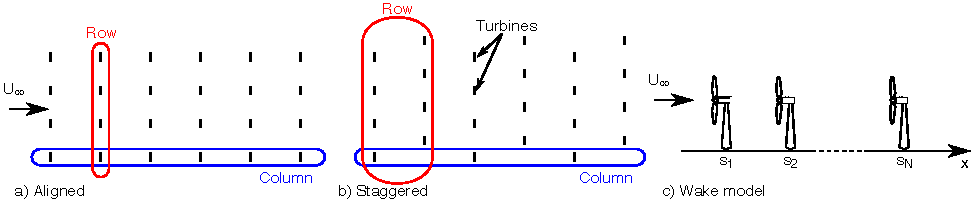
\includegraphics[width=\textwidth]{./fig/wake_model_final.pdf}
\caption{Diagrams of (a) an aligned and (b) a staggered wind farm showing definitions of rows and columns and (c) a wake model showing definitions of the streamwise coordinate x and the turbine locations $\text{s}_\text{n}$. The aligned and staggered wind farms have the same number of turbines, but the staggered arrangement has twice as many columns and double the distance between rows.}
\label{fig:wake_model}
\end{figure}

Since we are only considering the unyawed case, the forcing is only in the steamwise direction and the index notation can be dropped from the discussion of Section~\ref{sec:dynwake-wakemodel}. Instead, the equations are indexed by turbine row $n$ and some equations must be written in terms of the distance from the turbine rotor $x-s_n$. We follow the simplified approach of the Jensen model~\cite{Katic1986a} by first computing the wake deficit velocity $\delta u_n(x,t)$ for each turbine $n$ as if each turbine was on its own, i.e. based on the same freestream velocity $U_\infty$. As in Section~\ref{subsec:dynwake-conclusions}, time-dependency is included by allowing the  thrust coefficient of each turbine  to depend on time  and describing the associated evolution of the wake deficit velocity $\delta u_n(x,t)$ based on the momentum equation. The velocity deficits of all turbines are then superposed using the common ``square-superposition" approach~\cite{Katic1986a}. 

For completeness, we present the one-dimensional wake model for unyawed turbines in a wind farm with all relevant details. The streamwise velcity deficit of the $n$-th turbine is governed by
\begin{equation}
\label{eq:delta_un}
\frac{\partial \delta u_n}{\partial t} + U_\infty \frac{\partial \delta u_n}{\partial x} = -w_n(x) \delta u_n(x,t) + f_n(x,t),
\end{equation}
where $w_n(x)$ is the wake decay function and $f_n(x,t)$ is a forcing function used to account for the effect of the turbine on the flow field. The wake decay function
\begin{equation}
w_n(x) = 2 \frac{U_\infty}{d_n(x)} \frac{d}{dx}d_n(x)
\end{equation}
is determined by the wake diameter normalized by the rotor diameter 
\begin{equation}
d_n(x) = 1 + k_n\ln \left(1 + \exp \left[\frac{x-s_n-2\Delta_w}{R}\right]\right),
\end{equation}
where $k_n$ is the wake expansion coefficient of the $n$-th turbine. The forcing function is specified as
\begin{equation}
\label{eq:forcing}
f_n(x,t) = 2 U_\infty^2  \frac{C_{Tn}'(t)}{4 + C_{Tn}'(t)} G(x-s_n),
\end{equation}
where $G(x)$ is the same Gaussian function in~\eqref{eq:gaussian}.

Equations~\eqref{eq:delta_un}--\eqref{eq:forcing} above describe the time-varying behavior of a wake generated by a single turbine row. The squared deficits~\cite{Katic1986a} are superposed to calculate the streamwise velocity at position $x$ and time $t$
\begin{equation}
\label{eq:u}
u(x,t) = U_\infty - \left(\sum_{m=1}^N \delta u_m^2(x,t)\right)^{1/2}.
\end{equation}
The estimated velocity at the $n$-th turbine row $\hat{u}_n$ is then found using
\begin{equation}
\label{eq:estimated_velocity} 
\hat{u}_n (t) = \int_0^L  u(x,t) G(x - s_n) \, dx.
\end{equation}
Note that we use the same Gaussian shape function as an integration kernel for this superposition in order to maintain smoothness in the adjoint fields discussed in Chapters~\ref{chap:rhc} and~\ref{chap:rhc2}. Finally, the total estimated power $\hat{P}_n$ of the $M$ turbines in row $n$ is
\begin{equation}
\label{eq:estimated_power_row}
\hat{P}_n =  M \frac{1}{2}\rho \frac{\pi D^2}{4} C'_{Pn} \hat{u}_n^3.
\end{equation}
where $C'_{Pn}$ is the local power coefficient. 

Using simple momentum theory (see Section~\ref{subsec:methods-les-turbine}), which assumes idealized conditions, $C_P' = C_T'$.  These idealized conditions assume that the electrical power generated by the turbine is proportional to the power extracted from the flow and the control actions do not significantly affect the aerodynamic efficiency of the blades~\cite[Appendix A]{Goit2015a}. Aerodynamic losses could also be taken into account by reducing the local power coefficient $C_P' \approx \alpha C_T'$ by a constant factor $\alpha$~\cite{Stevens2014b}. For example, a wind turbine operating at a thrust coefficient of $C_T = 0.75$ and $C_P = 0.45$ would use $\alpha = 0.8$. 

This formulation recovers the classical steady-state Jensen model for a single column if one uses a steady local thrust coefficient and appropriate expressions for the shape function and the normalized wake diameter. Specifically, the use of a Dirac delta function instead of the Gaussian $G(x-s_n) \to \delta(x-s_n)$ restores the step change in velocity deficit at the turbine. The wake expansion function $d_n(x) = 1 + 2k_n(x-s_n)/D$ restores the unmodified linear wake growth. Taken together, the above equations yield a nonlinear model with $N$ inputs $C_{Tn}'$, $N$ outputs $\hat{P}_n$, and a set of $N$ PDEs. While this system is infinite-dimensional, seeking solutions to this model using finite-differencing; this leads to 1,750 states for the relatively coarse grid resolution of 28 m and wind farm size $N=7$ used in this study.

\subsection{Validation --- Wind farm startup}
\label{subsec:dynwake-1d-validation}
We now validate the model by comparing the local velocities at each row estimated by the time-varying one-dimensional wake model to velocities obtained from LES of wind farms at startup. These simulations were performed by Pieter~Bauweraerts using KU Leuven's LES code SP-WIND~\cite{Goit2015a, Calaf2010a, Munters2016a}, which shares many numerical details with LESGO.  Unlike LESGO, however, it uses four-stage fourth-order Runge-Kutta time integration, fourth-order energy conserving finite differencing in the vertical direction. SP-Wind uses shifted periodic boundary conditions for the precursor domain~\cite{Munters2016a} to reduce the production of unrealistically long streamwise streaks in the precursor domain. The Smagorinsky subgrid-stress model~\cite{Smagorinsky1963a} with wall damping is used.

For the startup validation, the prescribed surface roughness parameter is $z_{0} = 0.1$ m. Both the wind farm and the precursor domains use the same constant pressure gradient yielding an average of $U_\infty = 9$ m/s at hub height. The precursor domain and wind farm domains have lengths of $13.3$ km in the streamwise direction, 5 km in the spanwise direction, and 1 km in the vertical direction. The number of gridpoints in each domain is $576 \times 256 \times 128$, which corresponds to grid sizes of 23 m $\times$ 20 m $\times$ 8 m in the streamwise, spanwise, and vertical directions, respectively. In the precursor domain, the recycling region is the first 8.7 km and the fringe forcing region is the last 2 km. In the wind farm domain, the first row of turbines is located 1.4 km from the beginning of the domain and the fringe forcing region is the last 2 km. 

 The simulations are started from a fully-developed neutral atmospheric boundary layer, to which the wind farm actuator disk forcing is introduced as a step change in $C_T'$ from 0 to 1.33. Both aligned and staggered arrangements are considered. The aligned wind farm is composed of $N=14$ rows of $M=10$ turbines. Each turbine has a rotor diameter of $D=100$ m and a hub height of 100 m. The spacing between turbines is $7D$ in the streamwise direction and $5D$ in the spanwise direction. The staggered wind farm uses the same configuration with alternating rows offset by half the spanwise spacing in the spanwise direction. This can be viewed as modeling only one streamwise column of turbines and multiplying by the number of columns. Startup is simulated for 20 different initial conditions, which are generated by the same atmospheric boundary layer simulation but separated by approximately one wind farm flow-through time to produce sufficient independence between inflow conditions. Averaging over spanwise columns and 20 simulations results in an average over a total of 200 samples.

\begin{figure}[h]
\centering
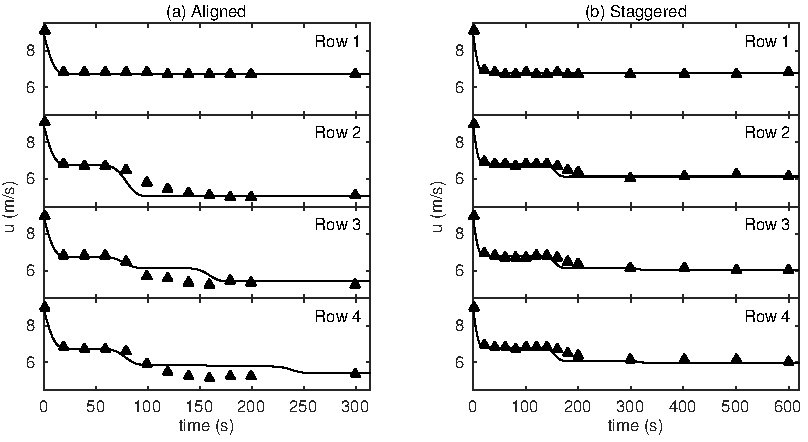
\includegraphics[width=\textwidth]{./fig/startup.pdf}
\caption{Comparison of wake model (---) and LES  averaged over spanwise rows and 20 simulations ($\blacktriangle$) for a wind farm at startup. Local turbine velocities of rows 1--4 are shown as a function of time for (a) aligned and (b) staggered wind farms. The initial decline in velocity in each row is produced by the startup induction of the turbines. Subsequent declines in velocity at downstream rows are produced as the wakes from upstream turbines impact the turbine rotor plane.}
\label{fig:compare}
\end{figure}

The wake model is evaluated numerically using four-stage fourth-order Runge-Kutta time integration with third-order upwind biased spatial discretization, 28 m grid spacing, and a CFL number of 0.99. The parameters $U_\infty$ and $k_n$ must be chosen to describe the flow conditions in the atmospheric boundary layer. In this validation, these parameters are chosen such that the estimated velocities of the steady-state version of the wake mode match the time-averaged velocities from the same wind farm configurations operating at a constant $C_T'=1.33$. The inlet velocity is chosen as $U_\infty = \overline{u}_1(4+C_T')/4$, where $ \overline{u}_1$ is the time-averaged local velocity of the first row of turbines as measured in LES. This results in $U_\infty = 8.93$ m/s for the aligned case and $U_\infty = 9.04$ m/s for the staggered case. The wake expansion coefficients $k_n$ are chosen so that the predicted velocity at downstream rows match the time-averaged LES measurements. The wake model for the staggered case uses only seven rows of turbines with twice the streamwise spacing. 

The time evolution of the velocities at rows 1--4 for a wind farm startup beginning at $t=0$ is shown in Figure~\ref{fig:compare}, where the estimated turbine velocity $\hat{u}_n$ is compared to the streamwise velocity at the center of the turbine rotor averaged over 20 LES. As the model farm and LES start up, the wind speed in all rows initially declines exponentially from the inlet velocity $U_\infty$ to the expected rotor-averaged velocity $4/(4+C_T') U_\infty$. Subsequent declines in velocity at downstream rows are produced as the wakes from upstream turbines impact the turbine rotor plane. Figure~\ref{fig:compare} shows that the wake model captures the wind farm startup response behavior, although there are some obvious differences between the predictions and measurements. For example, assuming a constant advection speed of $U_\infty$ leads to an under-estimate of the advection time between turbines. Maintaining the nonlinear advection speed produces a more accurate wind speed prediction in the wake; however, the concomitant nonlinearity would lead to added complexity and cost in the subsequent control design and implementation. 

\section{Conclusion}
\label{subsec:dynwake-conclusions}
In this chapter, we first developed a simple one-dimensional PDE model of the velocity deficits $\delta u_i(x,t)$ in the wake behind a turbine. This model requires as input the results from inviscid flow past a turbine to specify the forcing term in the PDE. We then apply the model to predict the time evolution of velocity deficits in regularly-arranged wind farms where each turbine is unyawed and compare the model to ensemble and spanwise-averaged large eddy simulations of a wind farm at startup. The performance in Figure~\ref{fig:compare} suggests that the dynamic behavior is adequately captured for a closed-loop control design, where the feedback accommodates small errors. Therefore, this model will be used in the next section for designing controllers for secondary frequency regulation. 

\chapter{Wind turbines in yaw: a lifting line approach}
\label{chap:yaw}
\chaptermark{Yawed wind turbines}

Yawing of wind turbines has the potential to increase wind farm power production by deflecting wakes away from downstream turbines~\cite{Fleming2015a, Bastankhah2016a, Branlard2016a, Howland2016a}. Dynamic yawing can also be used to regulate wind farm power production for improved integration in power systems~\cite{Aho2012a, Shapiro2017a}. Despite these promising emerging applications, a practical, yet accurate, aerodynamic theory is missing. Specifically, accurately predicting, from first principles, the magnitudes of the transverse velocity and the axial velocity deficit, the circulation of the shed counter-rotating vortex pair~\cite{Bastankhah2016a, Howland2016a}, and the skewness of the wake downstream remains a challenge.

Inviscid models of the region near the rotor of un-yawed turbines have played an important role in wind turbine modeling. Axial momentum theory and the vortex cylinder model have been used to derive the celebrated Betz limit and predict the initial wake velocity deficit~\cite{Glauert1935a, Burton2011a}. Blade element momentum theory \cite{Burton2011a,Hansen2008a} and vortex system models~\cite{Glauert1935a, Branlard2015a} have been used to predict the distribution of loads and velocity deficits in the wake. 
Such inviscid results are often used as initial conditions for models describing the turbulent wake downstream of the turbine (e.g. Chapter~\ref{chap:dynwake})~\cite{Jensen1983a, Frandsen2006a}.

In contrast, the arguments used in models of un-yawed turbines cannot always be straightforwardly applied to derive accurate predictions for yawed turbines. For example, the low pressure within the cores of the counter-rotating vortices results in a non-vanishing transverse pressure force on the streamtube. As a result, momentum balance arguments~\cite{Burton2011a, Jimenez2010a}, Glauert's proposed equation for the axial induced velocity through the rotor~\cite{Glauert1926a}, and the skewed elliptic vortex cylinder model~\cite{Coleman1945a,Branlard2016a} lead to conflicting results that do not always agree with the data. Resolving the significant differences among these models is vital for properly setting the initial conditions for models of the turbulent wake of yawed turbines.

In Section~\ref{sec:yaw-adm}, a model for the predominantly inviscid region near the rotor of a yawed actuator disk is proposed that agrees with measurements from numerical simulations. A key insight of this approach is to regard a yawed actuator disk as a lifting surface with an elliptic distribution of transverse lift. Then, Prandtl's lifting line theory~\cite{Milne-Thomson1973a} is used to predict the initial constant transverse velocity and the strength of the counter-rotating vortex pair. The transverse velocity is then combined with streamwise momentum theory to predict the induced velocity through the rotor and the initial streamwise velocity deficit. In Section~\ref{sec:yaw-wakemodel} these results are used as initial conditions in a model for the evolution of a turbulent wake far downstream of a yawed turbine.

\section{The yawed actuator disk as an elliptically loaded lifting line}
\label{sec:yaw-adm}
In actuator disk theories, wind turbines can be treated as porous disks that exert a thrust force perpendicular to the rotor area on the flow field (see Section~\ref{subsec:methods-les-turbine}). Figure~\ref{fig:yawed-actuator-disk} defines the  coordinate system $\mathbf{x} = (x,y,z)$ with the unit vectors $\boldsymbol{i}$, $\boldsymbol{j}$, and $\boldsymbol{k}$ aligned with the incoming flow velocity $\mathbf{U}_\infty = U_\infty \boldsymbol{i}$. The coordinate system $\mathbf{x}' = (x',y',z')$ is aligned with the unit normal of the actuator disk $\mathbf{n} = \cos \gamma \, \boldsymbol{i} + \sin \gamma \, \boldsymbol{j}$, where $\gamma$ is the angle between $\mathbf{U}_\infty$ and $\mathbf{n}$. The actuator disk forcing per unit volume 
\begin{equation}
\mathbf{f}(\mathbf{x}) = T \, \mathcal{R}(\mathbf{x}) \, \mathbf{n}
\end{equation}
equally distributes the total thrust force $T$ in the direction $\mathbf{n}$, where the area fraction function is defined as \begin{equation}
\mathcal{R}(\mathbf{x}) = \frac{1}{\pi R^2} \delta (x') H(R - \vert r' \vert),
\end{equation}
$\delta(x)$ is the Dirac delta function, $H(x)$ is the Heaviside (unit step) function, $r'^{\,2} = y'^{\,2} + z'^{\,2}$, and $R=D/2$ is the radius of the disk. (Note that the area fraction function here differs from the indicator function defined in Section~\ref{subsec:methods-les-turbine}.) The area fraction function is non-zero only within a disk of infinitesimal thickness that encloses the rotor swept area. The velocity field is denoted by $\mathbf{u}(\mathbf{x})$, and the fluid density is denoted by $\rho$. The total thrust force can be written in terms of the inflow velocity $U_\infty$ and thrust coefficient $C_T$ or the disk-averaged velocity normal to the disk 
\begin{equation}
u_d= \int \mathbf{u}(\mathbf{x}) \cdot \mathbf{n} \, \mathcal{R}(\mathbf{x}) \, d^3 \mathbf{x}
\end{equation}
and local thrust coefficient $C_T'$~\cite{Calaf2010a} as follows
\begin{equation}
\label{eq:thrust}
T = -\frac{1}{2} \rho \pi R^2  C_T U_\infty^2 \cos^2\gamma  = -\frac{1}{2} \rho \pi R^2 C_T' u_d^2.
\end{equation}

\begin{figure}
\begin{center}
\subimport{./fig/}{yawed-actuator-disk.pdf_tex}
\end{center}
\caption{\label{fig:yawed-actuator-disk} An actuator disk with radius $R$ yawed at an angle $\gamma$.}
\end{figure}

As in models of the flow around un-yawed actuator disks, we divide the flow into two regions, as shown in Figure~\ref{fig:yawed-actuator-disk-wake}. We first consider the predominantly inviscid region near the disk. The description of this region can then be used as an initial condition for models of the wake, where turbulent mixing dominates.  In the inviscid region, we first employ the vorticity equation to avoid dealing with pressure fields, which is equivalent to considering the fate of circulation. The appropriate framework is the Prandtl lifting line theory~\cite{Milne-Thomson1973a}, which can be used to predict the transverse velocity, shed circulation, and strength of the counter-rotating vortex pair. 

\begin{figure}
\begin{center}
\subimport{./fig/}{yawed-actuator-disk-wake.pdf_tex}
\end{center}
\caption{\label{fig:yawed-actuator-disk-wake} Sketch of the two regions downstream of the rotor: the inviscid region of streamwise velocity deficit, shown in blue, with a counter-rotating vortex pair with circulation $\pm\Gamma_0$, superimposed in green, and the expanding turbulent wake region, shown as dashed lines, developing downstream of the inviscid near-disk region.}
\end{figure}

There is an natural analogy between the yawed actuator disk and Prandtl's lifting line theory for finite wings~\cite{Milne-Thomson1973a}. First, let us consider a two-dimensional airfoil in a fluid with density $\rho$ inclined at an angle $\gamma$ to the freestream velocity $U_\infty$, as shown in Figure~\ref{fig:naca-coordinates}. Let $y$ denote the direction of lift and $z$ denote the right-handed direction of circulation in the $x$-$y$ plane. The flow around the airfoil, shown in Figure~\ref{fig:naca-streamlines}, is composed by the superposition of the freestream uniform velocity field and an ideal vortex with circulation $\Gamma$. This circulation is defined to satisfy the Kutta condition, which specifies that the velocity at the trailing edge of the airfoil must be smooth~\cite[pg. 211]{Houghton2013a}, and therefore only depends freestream velocity, angle of attack, and the geometry of the airfoil itself. The Kutta-Joukowsky theorem then gives the relationship between the circulation and the resulting lift~\cite[pg. 92]{Milne-Thomson1973a}.\footnote{Milne-Thomson denotes the inflow velocity pointing in the negative $x$ direction, the span along the $y$ direction, the lift in the negative $z$ direction, and the circulation $\Gamma$ in the positive $y$ direction. Our nomenclature differs, with the inflow velocity $U_\infty$ pointing in the positive $x$ direction, the span $2R$ along the $z$ direction, the lift in the positive $y$ direction, and the circulation $\Gamma$ in the positive $z$ direction. As a result, the (right-handed) circulation distribution switches sign in our convention.}
\begin{equation}
\label{eq:kuta-joukowsky}
l = - \rho U_\infty \Gamma
\end{equation}

\begin{figure}
\begin{center}
\subimport{./fig/}{naca-coordinates.pdf_tex}
\end{center}
\caption{\label{fig:naca-coordinates} A two-dimensional airfoil in a fluid with freestream velocity $U_\infty$. The streamwise coordinate $x$ is aligned with the freestream velocity, and the lift is aligned with $y$. The circulation is defined to be right-handed, and is therefore negative in this flow. Adapted from ~\cite{Belisle2008a}.}%https://en.wikipedia.org/wiki/File:Streamlines_around_a_NACA_0012.svg
\end{figure}

Now consider a finite airfoil with a span length of $2R$, as shown in Figure~\ref{fig:finite_airfoil}. Prandtl's lifting line theory considers each spanwise section using the two-dimensional theory and distributes the distribution of circulation $\Gamma(z)$ as a line along the spanwise coordinate $z$. The resulting lift distribution per unit span $l(z)$ is given based on the Kuta-Joukowski theory~\eqref{eq:kuta-joukowsky}, giving a total lift of~\cite[pg. 197]{Milne-Thomson1973a}
\begin{equation}
L = \int_{-R}^R l(z) \, dz = - \int_{-R}^R \rho U_\infty \Gamma(z) \, dz.
\end{equation}
Since vortex lines must be closed or terminate at a boundary, the vortex line forms a vortex line that begins at the wing and ends at a starting vortex behind the airfoil. The corresponding strength of the vortex lines shed from the airfoil is $d\Gamma/dz$~\cite[pg. 195]{Milne-Thomson1973a}. This trailing vortex sheet, however, is unstable and rolls up into two large counter-rotating vortices in the wake of the airfoil~\cite[pg. 185]{Milne-Thomson1973a}. The downwash $w(z)$ [\footnote{Using our coordinate system, the downwash is negative since the vertical coordinate $y$ is in the positive lift direction}, just behind the trailing edge of the airfoil, generated by the circulation system is found using the Biot-Savart law~\cite[pg. 197]{Milne-Thomson1973a}] 
\begin{equation}
\label{eq:downwash}
w(z) = \frac{1}{4\pi}\int_{\eta=-R}^{\eta=R} \frac{1}{z-\eta} \, d \Gamma.
\end{equation}


\begin{figure}
\begin{center}
\subimport{./fig/}{naca-streamlines.pdf_tex}
\end{center}
\caption{\label{fig:naca-streamlines} Streamlines around an airfoil with uniform freestream velocity and circulation satisfying the Kuta condition. Adapted from ~\cite{Belisle2008a}.}%https://en.wikipedia.org/wiki/File:Streamlines_around_a_NACA_0012.svg
\end{figure}


\begin{figure}
\begin{center}
\subimport{./fig/}{finite_airfoil.pdf_tex}
\end{center}
\caption{\label{fig:finite_airfoil} Finite airfoil with a span of $2R$ with a trailing vortex sheet that rolls up into two counter-rotating vortices.}%https://en.wikipedia.org/wiki/File:Streamlines_around_a_NACA_0012.svg
\end{figure}

In the analogy between the yawed wind actuator disk and the lifting line theory, the elliptically loaded finite airfoil is an important special case. Let the circulation along the span be given by an elliptic distribution
\begin{equation}
\label{eq:elliptic-circulation}
\left( \frac{\Gamma(z)}{\Gamma_0} \right)^2 + \left( \vphantom{ \frac{\Gamma(z)}{\Gamma_0}} \frac{z}{R} \right)^2  =  1,
\end{equation}
with a maximum circulation magnitude $\Gamma_0$ at the center of the span $z=0$, as shown in Figure~\ref{fig:elliptic-loading}. The classic elliptic circulation distribution is generated using an elliptic chord distribution, but it can also be created by varying airfoil sections and twist angle along the span. Using the coordinate transformation $z=-R \cos \theta$, the circulation distribution is~\cite[pg. 200]{Milne-Thomson1973a}
\begin{equation}
\Gamma(z) = -\Gamma_0 \sin \theta.
\end{equation}
Letting $\eta = -R\cos \phi$, the downwash is
\begin{equation}
w(z) = -\frac{1}{4\pi} \int_0^\pi \frac{\Gamma_0 \cos \phi}{ R (\cos \phi - \cos \theta)} \, d\phi = -\frac{\Gamma_0}{4R},
\end{equation}
independent of $z$. The elliptically loaded wing is a special case with constant downwash and minimized induced drag~\cite[pp. 201, 209]{Milne-Thomson1973a}. The strength of the counter-rotating vortices shed shed behind the wing are
\begin{equation}
\label{eq:gamma_shed}
\int_{-R}^{0} \frac{d\Gamma}{dz} \, dz = -\int_{0}^{R} \frac{d\Gamma}{dz} \, dz = \Gamma_0.
\end{equation}
and the distance between them is $\pi R/2$~\cite[pg. 209]{Milne-Thomson1973a}.

\begin{figure}
\begin{center}
\subimport{./fig/}{elliptic-loading.pdf_tex}
\caption{\label{fig:elliptic-loading} Elliptic spanwise circulation distribution between $z=-R$ and $z=R$ with a maximum circulation $-\Gamma_0$.}
\end{center}
\end{figure}

\begin{figure}[b]
\begin{center}
\subimport{./fig/}{chord.pdf_tex}
\caption{\label{fig:chord} Chord length $c(z)$ of the actuator disk with radius $R$ at a spanwise location $z$. }
\end{center}
\end{figure}
%
The yawed actuator disk can be viewed as an inclined lift-generating surface, akin to the finite airfoil discussed above, with a total span of $2R$ and a chord length $c(z)$ that varies along the vertical direction $z$. Geometrically, the chord length $c(z)$ is the length of the line segment between the two outer points of the disk at a point $z$, as shown in Figure~\ref{fig:chord}, expressed mathematically as 
\begin{equation}
\label{eq:chord}
\left(\frac{c(z)}{2}\right)^2 + z^2 = R^2.
\end{equation}
To apply lifting line theory, the associated lift force can be thought to be distributed along a line segment through the origin between $z=-R$ and $z=R$, as shown in Figure~\ref{fig:lifting-line}.
The lift is found by decomposing the thrust force into a streamwise force along the $x$-axis and a transverse force along the $y$-axis
\begin{equation}
\boldsymbol f (\mathbf{x}) = T \cos \gamma \, \mathcal{R}(\mathbf{x}) \boldsymbol{i} + T \sin \gamma \, \mathcal{R}(\mathbf{x}) \boldsymbol{j} 
\end{equation}
The total transverse force that the fluid exerts on the actuator disk, which we refer to as the ``transverse lift," is therefore
\begin{equation}
L = - T \sin \gamma.
\end{equation}
Since the lift distribution imposed by the fluid on the actuator disk is uniformly distributed over the disk, the lift per unit span $l(z)$ is equal to the lift per unit area $L/\pi R^2$ times the chord length $c(z)$
\begin{equation}
l(z) = \frac{L}{\pi R^2} c(z).
\end{equation}
At $z=0$ the chord length is $2R$, the lift has a maximum value of 
\begin{equation}
\label{eq:l0}
l_0 = \frac{2L}{\pi R} = \frac{-2T\sin\gamma}{\pi R} =   \rho R  C_T U_\infty^2 \cos^2 \gamma \sin \gamma.
\end{equation}

\begin{figure}
\begin{center}
\subimport{./fig/}{lifting-line.pdf_tex}
\caption{\label{fig:lifting-line} The lifting line segment through the origin between $z=-R$ and $z=R$ has a lift force per unit span of $l(z)$. At $z=0$ the lift is $l_0$ and the circulation is $\Gamma_0$.}% (b) The inviscid streamtube in the near-rotor region  of a yawed actuator disk. The rotor region, assumed to be an elliptic cylinder, is between the dotted lines.}
\end{center}
\end{figure}

Using the geometric relationship~\eqref{eq:chord}, the resulting distribution of circulation along the span $\Gamma(z)$, which is related to the lift by the Kuta-Joukowsky theorem~\eqref{eq:kuta-joukowsky}, has an elliptic distribution~\eqref{eq:elliptic-circulation}. The maximum circulation magnitude is related to the maximum lift~\eqref{eq:l0} 
\begin{equation}
\label{eq:gamma0}
\Gamma_0 = - \frac{l_0}{\rho U_\infty} = -R \, C_T U_\infty \cos^2\gamma \sin \gamma.
\end{equation}
As with an elliptically loaded wing, vortex filaments with a strength per unit span $d\Gamma/dz$ are shed and roll up into counter-rotating trailing vortices at the top and bottom of the disk~\eqref{eq:gamma_shed} with strength
\begin{equation}
\Gamma_\text{bottom} = \Gamma_0 \qquad \qquad \Gamma_\text{top} = - \Gamma_0.
\end{equation}
The downwash is therefore given by the maximum circulation magnitude~\eqref{eq:downwash}
\begin{equation}
\label{eq:deltav0}
\delta v_0 = -\frac{\Gamma_0}{4R} = \frac{1}{4} C_T U_\infty \cos^2\gamma \sin \gamma.
\end{equation}

In addition to the transverse velocity derived, additional expressions are needed to fully describe the inviscid region near the yawed actuator disk. The induced velocity through the disk, as well as the streamwise velocity deficit in the wake, are derived using an approach similar to the un-yawed momentum theory~\cite{Glauert1935a, Burton2011a}. The streamtube through the rotor is used as a control volume and the velocity is assumed to be uniform across every cross section, as shown in Figure~\ref{fig:momentum-theory}. The velocities upstream of the rotor and at the end of the inviscid region (beginning of the wake) are denoted by $\mathbf{U}_\infty$  and $\mathbf{U}_w$, respectively. Also, at those locations we consider flow through vertical sections with area vectors, $\mathbf{A}_\infty = A_\infty \, \boldsymbol{i}$ and $\mathbf{A}_w = A_w \,\boldsymbol{i}$, defined in Figure~\ref{fig:momentum-theory}. The disk-averaged velocity $u_d$ through the disk area $A_d = \pi R^2$ and mass conservation yields 
\begin{equation}
u_d A_d = \mathbf{U}_\infty \cdot \mathbf{A}_\infty  =  \mathbf{U}_w \cdot \mathbf{A}_w,
\end{equation}
where the dots indicate inner products. The wake velocity is written as 
\begin{equation}
\mathbf{U}_w = (U_\infty - \delta u_0) \boldsymbol{i} - \delta v_0 \, \boldsymbol{j},
\end{equation}
where $\delta u_0$ is the streamwise velocity deficit and $\delta v_0$ is the transverse velocity magnitude specified by the lifting line theory in~\eqref{eq:deltav0}. 


\begin{figure}
\begin{center}
\subimport{./fig/}{momentum-theory.pdf_tex}
\caption{\label{fig:momentum-theory} The inviscid streamtube in the near-rotor region  of a yawed actuator disk. The rotor region, assumed to be an elliptic cylinder, is between the dotted lines.}
\end{center}
\end{figure}

The region of the streamtube cut by the actuator disk is treated as an elliptic cylinder with a cross sectional area of $A_d \cos \gamma$. Inside this volume, the upstream and downstream pressure are assumed to be constant at $p^+$ and $p^-$, respectively. The upstream and downstream  velocities are
\begin{align}
\mathbf{u}^+ &= u_d \cos^{-1}\gamma \, \boldsymbol{i} \\
\mathbf{u}^- &= u_d \cos^{-1}\gamma \boldsymbol{i} - \delta v_0 \, \boldsymbol{j},
\end{align}
respectively. The streamwise velocity through this region is assumed to be constant and is determined using mass conservation. The transverse velocity has a discontinuity at the disk, jumping from zero to the downwash $-\delta v_0$ behind the rotor region.

Assuming that the streamwise pressure force vanishes over the streamtube's surface, as in the un-yawed case~\cite{Glauert1935a}, the streamwise momentum equation  is
\begin{equation}
\label{eq:streamwise_momentum}
- \rho \, \mathbf{U}_\infty \cdot \mathbf{A}_\infty \,U_\infty + \rho\, \mathbf{U}_w \cdot \mathbf{A}_w\, (U_\infty - \delta u_0) = T \cos \gamma.
\end{equation}
The Bernoulli equation is then applied from far upstream to where $p=p^+$ and from where $p=p^-$ to further downstream of the turbine where $p$ recovers and the turbulent wake begins, as shown in Figure~\ref{fig:momentum-theory}. Assuming that $\delta v_0$ remains constant in the downstream part of the inviscid region, we write
\begin{align}
\label{eq:bernoulliup}
\frac{1}{2}  U_\infty^2   &= \frac{1}{2}   \left(\frac{u_d}{\cos \gamma}\right)^2 + \frac{p^+}{\rho~} \\
\label{eq:bernoullidown}
\frac{1}{2} \left(\frac{u_d}{\cos \gamma}\right)^2 + \frac{1}{2}  \delta v_0^2 +\frac{p^- }{\rho~}   &= \frac{1}{2}  (U_\infty - \delta u_0)^2 + \frac{1}{2}   \delta v_0^2.
\end{align}
%
Subtracting~\eqref{eq:bernoullidown} from~\eqref{eq:bernoulliup}, and noting that the pressure force opposes the streamwise thrust force, or drag, 
\begin{equation}
\left(p^+ - p^-\right) A_d   = -T,
\end{equation}
we obtain
%
\begin{equation}
\label{eq:bernoulli}
\frac{1}{2}  U_\infty^2 - \frac{1}{2}  (U_\infty - \delta u_0)^2  = -\frac{T}{\rho A_d}.
\end{equation}
%
Substituting the thrust force~\eqref{eq:thrust} and mass flow rate into~\eqref{eq:streamwise_momentum} and~\eqref{eq:bernoulli} yields two equations for the unknown disk-averaged velocity and streamwise velocity deficit
%
\begin{align}
2 \frac{u_d}{U_\infty} \frac{\delta u_0}{U_\infty} &= C_T \cos^3 \gamma \\
\frac{\delta u_0}{U_\infty} \left( 2 - \frac{\delta u_0}{U_\infty} \right) &= C_T \cos^2 \gamma.
\end{align}
%
Written in terms of the induction factor $a$, the solution is
\begin{align}
\label{eq:sys2}
u_d &= U_\infty \cos \gamma (1-a) \\
\delta u_0  &= 2 U_\infty a,
\end{align}
%
where the thrust coefficient is related to the induction factor by $C_T \cos ^2 \gamma = 4a(1-a)$. The induction factor can subsequently be written in terms of both the standard  and local thrust coefficients using the identity 
\begin{equation}
C_T U_\infty^2 \cos^2 \gamma = C_T' u_d^2
\end{equation}
according to
%
\begin{equation}
\label{eq:induction_factor}
a = \frac{C_T' \cos^2 \gamma}{4 + C_T' \cos^2 \gamma} = \frac{1}{2} \left(1 - \sqrt{1 - C_T \cos^2 \gamma} \right).
\end{equation}
The initial skewness angle is obtained from $\tan \alpha = -\delta v_0 / (U_\infty - \delta u_0)$.

\subsection{Validation --- Uniform inflow}
\label{subsec:yaw-validation}

\begin{figure}[b!]
\begin{center}
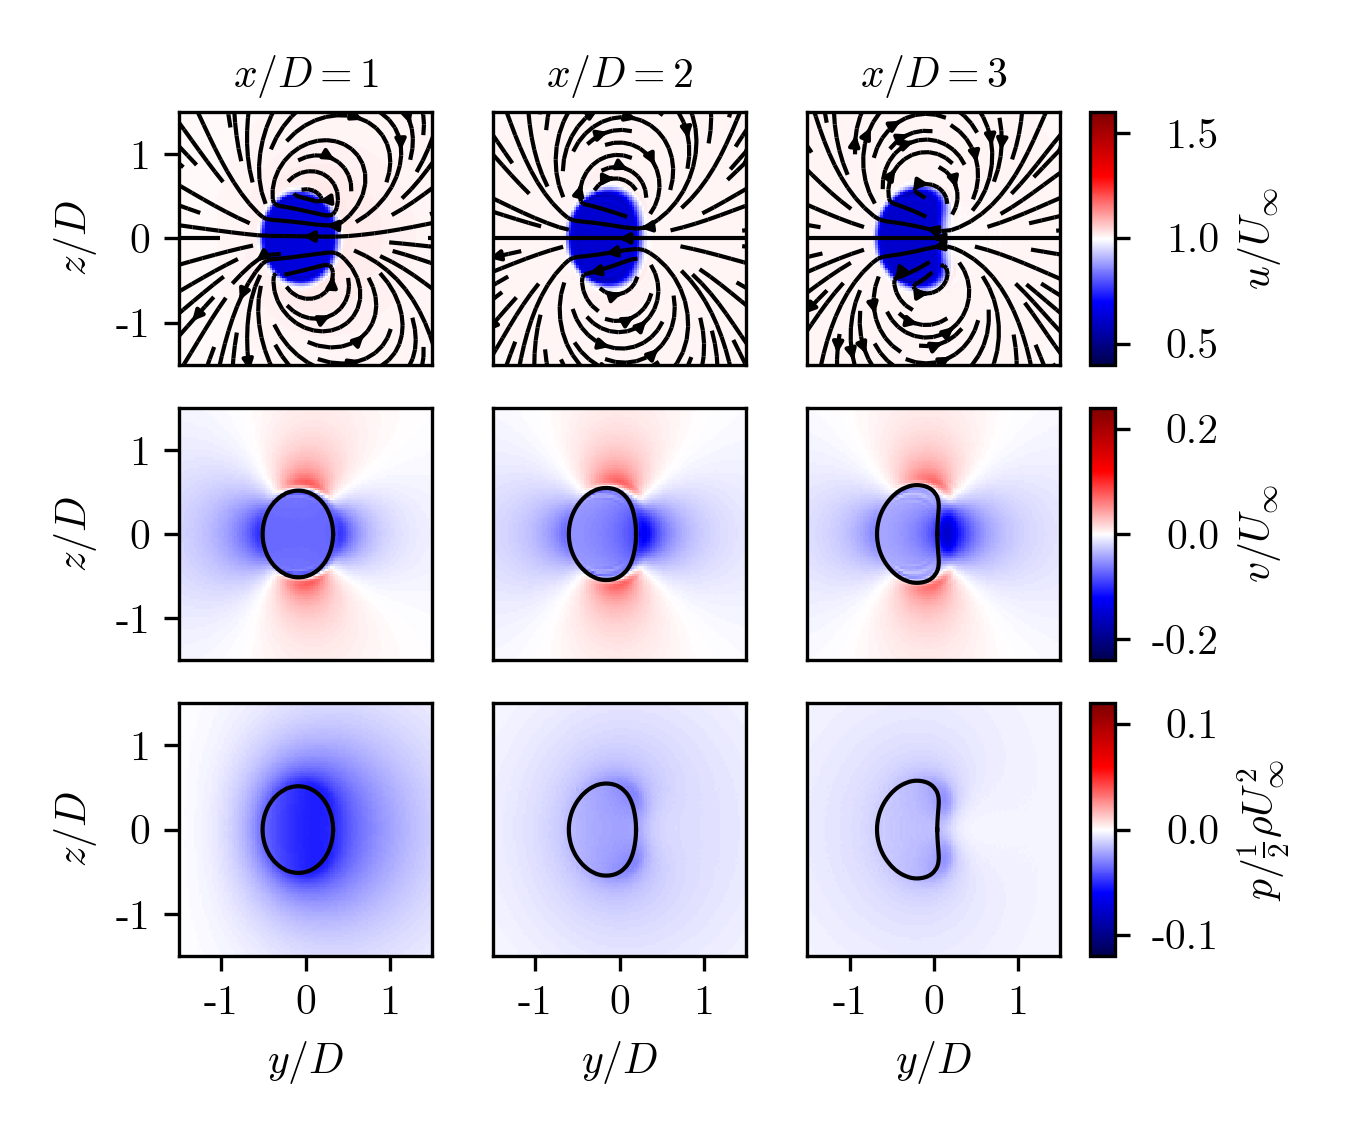
\includegraphics[width=\textwidth]{./fig/yzplane.png}
\caption{\label{fig:yzplane} Simulation results for $C_T' = 1.33$ and yaw angle $\gamma = 30^\circ$ in a domain $L_x/D=11.52$ and   $L_y/D=L_z/D=5.76$.
Shown are color contours of (top) streamwise velocity, (middle) transverse velocity, and (bottom) pressure at downstream locations $x/D = 1$, 2, and 3. Top panels  include streamlines in the $y$-$z$ plane. The transverse velocity and pressure plots show the outline of the wake, defined by the streamtube that passes the rotor at a radius of $r'=0.9R$.}
\end{center}
\end{figure}

In order to provide data to test predictions based on the proposed model above, numerical simulations of flow around a yawed actuator disk under uniform, laminar inflow are carried out using LESGO. A yawed actuator disk of diameter $D$ is placed in a domain of length $L_x=11.52D$ and cross-section size $L_y=L_z=5.76D$ using a total of \mbox{$384 \times 192 \times 192$} grid points. The center of the actuator disk is placed in the center of a $y$-$z$ plane $3.6D$ downstream of the domain inlet.  A uniform inflow velocity $U_\infty$ is applied using a fringe region forcing~\cite{Stevens2014a}.  Molecular viscosity is neglected and the Smagorinsky model is used  for numerical stability with $C_s = 0.16$. Since the flow in the bulk of the near-disk region of interest remains laminar and inviscid and the effect of the subgrid model is confined to the thin shear layer at the boundary of the wake, which is not included in the subsequent analysis, the details of the subgrid modeling are not important for present purposes. The simulations are insensitive to the choice of $C_s$, yielding the same results for $C_s = 0.08$. Various yaw angles $\gamma$ are considered. LESGO uses the local formulation of the thrust force with a local thrust coefficient $C_T'$~\cite{Calaf2010a}. The force is applied using the area fraction function filtered by a three-dimensional Gaussian (see~\eqref{eq:LESGO-Gaussian-kernel}) with a filter width $\sigma_{\mathcal{R}} = 1.5 h / \sqrt{12}$ proportional to the grid size $h = (\Delta x^2 + \Delta y^2 + \Delta z^2)^{1/2}$, where $\Delta x$, $\Delta y$, and $\Delta z$ are the grid spacings.  

Representative results at downstream distances $x/D = 1$, 2, and 3 are shown in  Figure~\ref{fig:yzplane} for $C_T' = 1.33$ and  $\gamma = 30^\circ$. A wake that stays laminar for a large portion of the domain is generated by the actuator disk forcing. At $x/D=1$ near the actuator disk, the wake forms an ellipse with uniform streamwise and transverse velocity components inside of the wake. The transverse component of the force generates the well known counter-rotating vortex pair~\cite{Howland2016a, Bastankhah2016a}, which curls the wake as it moves downstream, shown schematically in Figure~\ref{fig:yawed-actuator-disk-wake}. 

Further simulations are performed at yaw angles $\gamma = 10^\circ$, $20^\circ$, $30^\circ$, and $40^\circ$ and local thrust coefficients $C_T' = 0.8$, $1.0$, and $1.33$.
From these simulations, the spanwise circulation distribution $\Gamma(z)$ is evaluated numerically via integration along rectangular contours running from the inlet of the domain to $x=R$ and spanning the entire width of the domain. The circulation of each shed vortex $\Gamma_0$ is calculated at $x=R$ by averaging the circulation around two rectangular circuits spanning $|y| \le 3R$ and $ |z| \le 3R$. 

We seek to compare the measured results to~\eqref{eq:elliptic-circulation} and~\eqref{eq:gamma0}, for which the disk radius is an important parameter. The footprint of the applied force in the simulations extends slightly from the geometrically prescribed disk dimensions, owing to the use of a filtered area fraction function. To correct for the filtered geometric representation of the disk, the width of an equivalent top-hat filter~\cite{Pope2000a}  $\sqrt{12}\sigma_{\mathcal{R}}=1.5h$ ($h<<R$ is the grid size) is added to the diameter of the disk in~\eqref{eq:gamma0} when applying the inviscid model. The resulting effective radius is $R_*=R+0.75 h$, which leads to the predicted maximum circulation being given by $\Gamma_0 = -(R+0.75 h) \, C_T U_\infty \cos^2\gamma \sin \gamma$. The thrust coefficient is obtained from $C_T = C_T' u_d^2/ (U_\infty \cos \gamma)^2$, where the disk-averaged velocity $u_d$ is measured in the simulations.  As seen in the comparison shown in  Figures~\ref{fig:gamma}(a--b), the predicted circulation distribution and simulation results collapse for all $\gamma$ and $C_T'$ values tested. 

\begin{figure}
\begin{center}
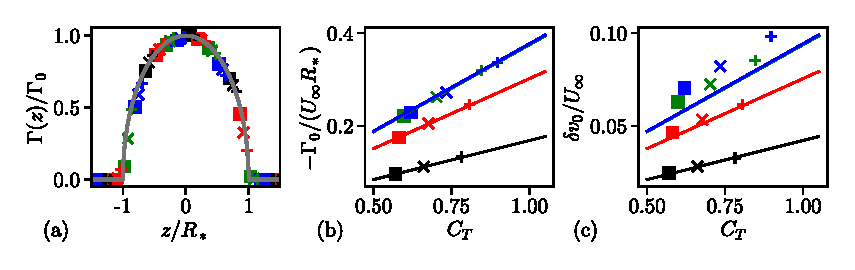
\includegraphics[width=\textwidth]{./fig/gamma.pdf}
\caption{\label{fig:gamma} Comparisons of (a) the measured circulation around the actuator disk (symbols) and the expected distribution from the elliptic lifting line $(1-z^2/R_*^2)^{1/2}$ (grey line), (b) the shed circulation of counter-rotating vortices measured at $x=R$ (symbols) and predicted by lifting line theory (lines), and (c)  the maximum $y$-$z$ planar-averaged transverse velocity measured in the streamtube (symbols) and transverse velocity predicted by lifting line theory (lines). Simulations are conducted with $\gamma = 10^\circ$ (black), $20^\circ$ (red), $30^\circ$ (green), and $40^\circ$ (blue) and $C_T' = 0.8$ ($\blacksquare$), 1.0 ($\times$), and 1.33 ($\bm{+}$). The theoretical values for $\gamma = 30^\circ$ and $40^\circ$ overlap in (b) and (c).}
\end{center}
\end{figure}

Next we compare the transverse velocity magnitude $\delta v_0$ with the model. To measure this value from simulations we take the maximum $y$-$z$ planar-averaged transverse velocity in the wake. The wake is defined as the streamtube passing through the disk at $r' = 0.9R$ to avoid including the thin shear layer near the actuator disk perimeter (results are quite insensitive to this choice). The downstream position of maximum transverse wake velocity occurs very near the disk, at $x \approx R$. Using the thrust coefficient obtained from \mbox{$C_T = C_T' u_d^2/ (U_\infty \cos \gamma)^2$}, we compare $\delta v_0 = \frac{1}{4} C_T U_\infty \cos^2\gamma \sin \gamma$ to simulation measurements in figure \ref{fig:gamma}(c). Again, excellent agreement is observed for various $\gamma$ and $C_T'$ combinations, with a slight underestimate at large $\gamma$. 


\begin{figure}
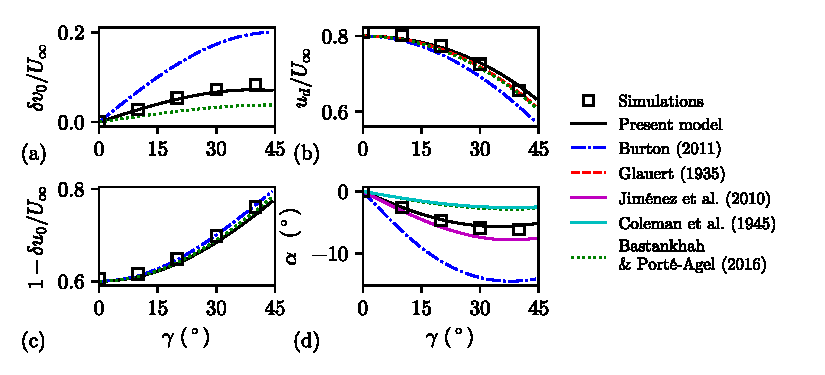
\includegraphics[width=\textwidth]{./fig/steady-uniform-1.pdf}
\caption{\label{fig:steady-uniform}Comparison of (a) transverse velocity $\delta v_0/U_\infty$, (b) disk-averaged velocity $u_d/U_\infty$, (c) streamwise velocity $1 - \delta u_0/U_\infty$,  and  (d) skewness angle $\alpha$ measured in simulations with $C_T' = 1.0$ (squares) with present theory (solid black line) and prior models (other lines).}
\end{figure}

The disk-averaged velocity, streamwise velocity deficit, transverse velocity, and skewness angle of the initial wake obtained from numerical simulations, the present model, and prior models are compared in Figure~\ref{fig:steady-uniform}. The velocity deficit $\delta u_0$ at the end of the inviscid region is obtained from the simulations as the maximum $y$-$z$ planar-averaged streamwise velocity deficit in the wake, which occurs at $x \approx 4D$. The maximum for $\delta u_0$ is further downstream than the maximum for $\delta v_0$ because $\delta u_0$ is strongly affected by streamwise pressure gradients. The transverse velocity prediction~\eqref{eq:deltav0} is expressed using the thrust coefficient $C_T = 16 C_T'/(4 + C_T'\cos^2\gamma)^2$ obtained from the induction factor equation~\eqref{eq:induction_factor}. Predictions for several of the features of the inviscid region are provided by earlier models. Momentum theory~\cite{Burton2011a} provides estimates for all quantities. Glauerts's~\cite{Glauert1926a} equation for the disk-averaged velocity was used by Coleman \textit{et al.}~\cite{Coleman1945a, Burton2011a} to predict the skewness angle of the wake. Bastankhah \& Port\'{e}-Agel~\cite{Bastankhah2016a} recently used momentum conservation, the Bernoulli equation, and approximations to Glauert's and Coleman's equations to predict the streamwise and transverse velocities behind the disk. Jimenez \textit{et al.}~\cite{Jimenez2010a} used momentum balance arguments to predict the initial wake deflection angle. 

Figure~\ref{fig:steady-uniform} shows that the present inviscid region model accurately predicts the quantities measured in simulations. In contrast, other models show significant disagreement in the skewness angle and transverse velocities. Momentum theory and Jim\'{e}nez's~\cite{Jimenez2010a} equation overestimate the skewness angle and transverse velocity magnitudes. The skewness angle magnitude predicted by Coleman~\cite{Coleman1945a}, and by extension the transverse velocity magnitude predicted by Bastankhah \& Port\'{e}-Agel~\cite{Bastankhah2016a}, are approximately half as large as those obtained in the simulations. While Coleman's~\cite{Coleman1945a} prediction may improve downstream as the wake is transformed by the counter-rotating vortex pair, this skewed elliptic vortex cylinder argument becomes less valid as a result of the curling. 

\section{Wake model for yawed turbines}
\label{sec:yaw-wakemodel}
An important application of the inviscid region theory described in the prior section is to determine an initial condition for models of the turbulent wake behind yawed turbines. We demonstrate the utility of the proposed inviscid region model by applying the predictions to the wake model of Section~\ref{sec:dynwake-wakemodel}.  Retaining the $u$ and $v$ components of the model, the velocity deficit source strengths, $S_1  = U_\infty \delta u_0$ and $S_2 = U_\infty \delta v_0$, are based on the inviscid model, where $\delta u_0$ and  $\delta v_0$ are given by~\eqref{eq:sys2} and \eqref{eq:deltav0}. This approach provides a smooth increase of the streamwise and transverse velocity deficits from zero upstream of the rotor to the desired `wake initial condition' downstream of the rotor region. 

The average streamwise velocity deficit $\delta u(x,t)$ is distributed using a Gaussian profile~\cite{Bastankhah2014a, Bastankhah2016a}, which along $z=0$ reads
\begin{equation}
\label{eq:u_model}
u(x,y,t) = U_\infty - \delta u(x,t) \, \frac{D^2}{8 \sigma_0^2} \,\exp \left(-  \frac{(y-y_c(x,t))^2}{2\sigma^2(x)} \right), 
\end{equation}
where the width of the Gaussian $\sigma(x) = \sigma_0 d_w(x)$ is proportional to the effective normalized wake diameter with a proportionality constant $\sigma_0$. The velocity deficits are found by integrating~\eqref{eq:preliminary_deficit}, and the wake centerline $y_c(x,t)$ is found by integrating the transverse velocity according to
\begin{equation}
\frac{\partial y_c}{\partial t} + U_\infty \frac{\partial y_c}{\partial x} = -\delta v(x,t).
\end{equation}
in the positive $x$ direction subject to $y_c = 0$ far upstream of the turbine. The negative sign occurs because $\delta v(x,t)$ is a deficit in our sign convention. 
Equation~\eqref{eq:u_model} is consistent with~\eqref{eq:area_velocity}; i.e. $\int_{0}^\infty (U_\infty - u) 2\pi \xi d\xi = A(x)\delta u(x,t)$, where the distance $\xi = y-y_c(x,t)$ is measured from the wake centerline at $y_c(x,t)$.
 
\begin{figure}[h!]
\begin{center}
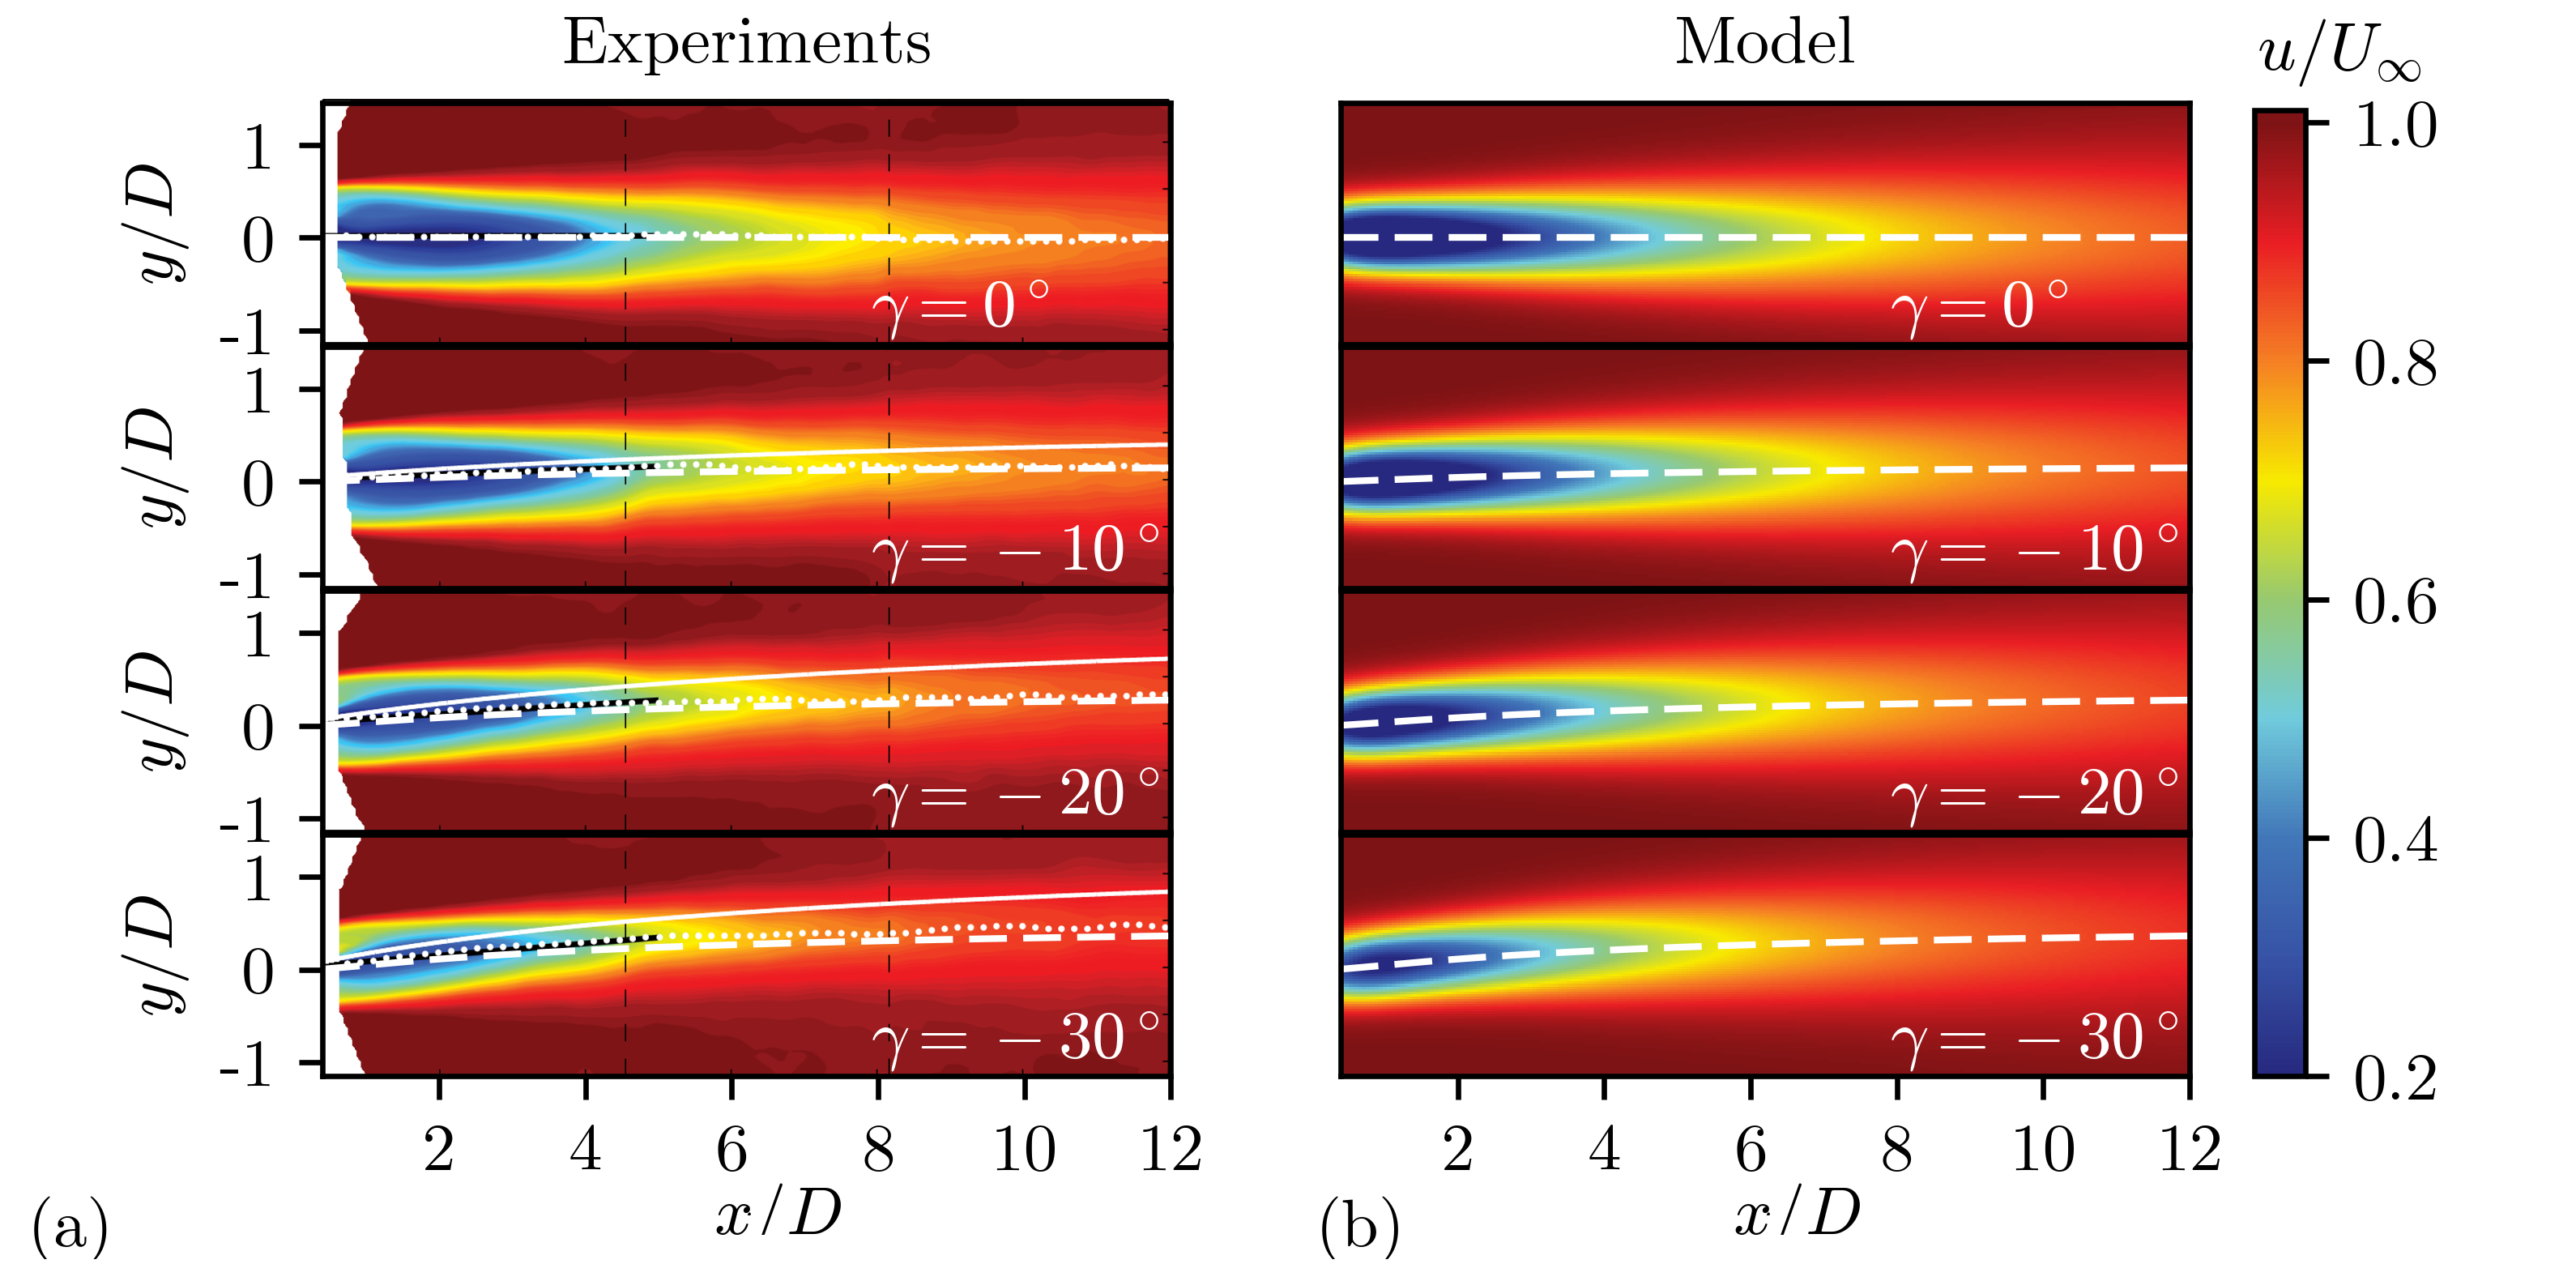
\includegraphics[width=\textwidth]{./fig/bastankhah_comparison_overlay.png}
\caption{\label{fig:far_wake} Hub-height color contour plots of streamwise velocity as (a) measured in experiments~\cite{Bastankhah2016a} and (b) predicted using the proposed model. 
Measured centerlines of the wake (dotted) are compared to the model of~\cite{Jimenez2010a} (solid) and the present model (dashed).  Experimental data in (a) adapted with permission from figure 3 of Bastankhah and Port\'{e}-Agel\cite{Bastankhah2016a}.}
\end{center}
\end{figure}

While this model includes possible time-dependence (e.g. the turbine's local thrust coefficient and yaw angle could change over time), in this chapter, we focus solely on the steady-state solution and compare it to the wind tunnel experiments of Bastankhah and Port\'{e}-Agel~\cite{Bastankhah2016a} that were performed under steady conditions. The steady-state version of this wake model, where time derivatives vanish and the solution found by integrating in $x$,
\begin{align}
\delta u(x) &= \frac{\delta u_0}{d_w^2(x)} \frac{1}{2}\left[1 + \mathrm{erf}\left(\frac{x}{\Delta_w \sqrt{2}}\right)\right]\\
\delta v(x) &= \frac{\delta v_0}{d_w^2(x)} \frac{1}{2}\left[1 + \mathrm{erf}\left(\frac{x}{\Delta_w \sqrt{2}}\right)\right]\\
y_c(x) &= \int_{-\infty}^x \frac{-\delta v(x')}{U_\infty} dx'
\end{align}
is compared to wind tunnel experiments by Bastankhah \&Port'{e}-Agel~\cite{Bastankhah2016a}. We use the experimental data for the un-yawed \mbox{($\gamma = 0^\circ$)} case to fit the two required  parameters $k_w$ and $\sigma_0$, obtaining very reasonable values $k_w=0.0834$ and  $\sigma_0 /D = 0.235$. 
The measured thrust coefficients of the rotating turbine (depending on the yaw angle, as reported by Bastankhah and Port\'{e}-Agel\cite{Bastankhah2016a}) are used to set the initial velocity deficits $\delta u_0$ and $\delta v_0$ in the model. Figure~\ref{fig:far_wake} compares the streamwise velocity deficit at hub height for $\gamma = 0^\circ$, $-10^\circ$, $-20^\circ$, and $-30^\circ$. The centerlines of the measurements are compared to the present model and the model of Jimenez \textit{et al.}~\cite{Jimenez2010a}. The proposed model is found to be in excellent agreement with the experiments, particularly the estimate of the centerline of the wake.  

\section{Conclusions}
\label{sec:yaw-conclusions}
Previous models for the inviscid region near a yawed actuator disk have generated conflicting predictions for the initial transverse velocity and skewness angle of the wake that fail to match actuator disk simulations. Accurate models for this inviscid region are vital for developing useful wake models for engineering design and control applications. In this chapter, we derive a new model of the flow in the inviscid region near the disk. It treats the yawed actuator disk as an elliptically loaded lifting line and uses Prandtl's lifing line theory to determine the initial transverse velocity deficit and magnitude of the counter-rotating vortex pair shed from the yawed actuator disk. Momentum conservation and Bernoulli's equation are then applied to determine the disk-averaged velocity and streamwise velocity deficit. The predictions are found to agree with numerical simulations and accurately estimating the initial transverse velocity.  We use the inviscid region predictions as initial conditions for a simple model of the flow field behind a yawed turbine and compare to experimental data. 
The newly proposed combined model for the inviscid and wake regions is remarkable for its simplicity and success at reproducing a variety of observations.


\chapter{Sensing and estimation}
\label{chap:estimation}
\chaptermark{Sensing and estimations}

The wake model discussed in Chapter~\ref{chap:dynwake} includes important aspects of wake advection, expansion, and interaction that have significant effects on the total wind farm power production. However, the model makes a number of simplifying assumptions, such as linear advection and neglecting spanwise wake interactions, and neglects natural variations in power production due to turbulence within the wind farm. There is also uncertainty in the model parameters, specifically the freestream velocity $U_\infty$ and the wake expansion coefficients $k_n$. 

Measurements that are readily available in existing wind farms may be able to correct many of these modeling errors. In addition to measurements of the power production at each turbine, velocity field and wind heading information can be obtained from a wide range of sensors. Sonic and propeller anemometers and wind vanes provide point source measurements of velocity~\cite{Pao2011a}, blade loads can be used to estimate wind alignment, wind shear, and wake locations~\cite{Bottasso2014a, Bottasso2018a}, and lidar measurements can be used to track wake positions~\cite{Raach2016a, Churchfield2016a}. Various measurements also can be combined to make estimates of other quantities such as the effective rotor-averaged wind speed~\cite{Knudsen2011a}.

All of the control designs considered in this thesis use power measurements for closed loop feedback. We consider two approaches that differ significantly in complexity. First, we consider a temporally damped correction term in Section~\ref{sec:estimation-damped} that does not directly correct model states or parameters. Instead, it provides a means of adjusting the current model output equation to improve the model based receding horizon control of Chapter~\ref{chap:rhc}. Second, we consider an ensemble based state and parameter estimation method in Section~\ref{subsec:estimation-ensemble-enkf}. At the cost of additional complexity, this approach provides online estimation of model parameters as well as direct state corrections to improve the model predictions.

\section{Temporally damped correction}
\label{sec:estimation-damped}
The simplest feedback used is a temporally-damped error correction term for the modeled rotor-averaged axial velocity. From the measured power production of the $m$-th turbine in the $n$-th row, the row-averaged power and row- and rotor-averaged wind velocities are defined as
\begin{equation}
\qquad P_n = \sum_{m=1}^M P_{nm}, \quad \text{and} \qquad \qquad u_n = \frac{1}{M}\left(   \sum_{m=1}^M u_{nm}^3  \right)^{1/3},
\end{equation}
where $u_{nm}$  is the velocity measured at the turbine in the $n$-th row and $m$-th column of the wind farm. The definition of the row-average velocity at the turbine disk is necessary to ensure that  the expression for the turbine output power $P_n = M \frac{1}{2} \rho \frac{\pi D^2}{4} C_{Tn}' u_{n}^3$ is satisfied. These measurements are used to calculate an error term $\epsilon_n$ and provide feedback by replacing Eq.~\eqref{eq:estimated_power_row} with
\begin{equation}
\hat{P}_n = M \frac{1}{2}\rho \frac{\pi D^2}{4} C_{Tn}' (\hat{u}_n + \epsilon_n)^3.
\end{equation}
The error correction at the current time $t_c$ is 
\begin{equation}
\epsilon_n(t) = \left(u_n(t_c) -  \hat{u}_n (t_c) \right) e^{-(t-t_c)/\tau}.
\end{equation}
The exponential decay accounts for the reduced  future accuracy of the error term in the prediction and is set to $\tau = 120$ s in the applicable results in Chapter~\ref{chap:rhc}.

While this feedback correction is simple to implement and incorporates the diminishing utility of  measurements further in the future, there are several deficiencies with this approach. First, the method assumes that the current measurement is perfectly accurate and ignores measurement error. Second, the corrections only affect the predictions at the turbine at which the measurement is taken. In the advective atmospheric boundary layer, past measurements at upstream turbines should affect the current estimate at downstream turbines. Finally, this method does not estimate the wake model parameters, which must be calculated in another way.

\section{Ensemble-based optimal estimation}
\label{sec:estimation-ensemble}

The second error correction method used is an ensemble based state and parameter estimation method employing an ensemble Kalman filter (EnKF)~\cite{Evensen2003a}. This approach provides online estimation of model parameters as well as state estimates. The EnKF approaches the properties of the standard Kalman filter (KF), but at significant computational savings. In this section, we first describe the canonical KF in Section~\ref{subsec:estimation-ensemble-kalman}. We then describe in Section~\ref{subsec:estimation-ensemble-enkf} the EnKF's approximation of the KF's error covariance matrix using an ensemble of state space representations and the associated forecast and analysis equations. Finally, we describe the details of the state and parameter estimation for the wake model of Section~\ref{sec:dynwake-1d} in Section~\ref{subsec:estimation-ensemble-wake} and validate the results using LES in Section~\ref{subsec:estimation-ensemble-validation}.

\subsection{The Kalman filter}
\label{subsec:estimation-ensemble-kalman}

The Kalman filter is a celebrated accomplishment of modern control theory that provides a rigorous method for estimating the state of a linear system using measurements and knowledge of the system's properties~\cite{Kalman1960a, Gelb1974a}. President Obama noted the profound impact of the Kalman filter upon awarding Rudolf Kalman the 2008 National Medal of Science 

\begin{quote}
for his invention of the ``Kalman filter," which was critical to achieving the Moon landings and creating the Global Positioning System and which has facilitated the use of computers in control and communications technology.~\cite{Obama2009a}
\end{quote}

In this thesis, we will follow the Kalman filter derivation of Gelb \textit{et al.}~\cite{Gelb1974a}. We consider linear, discrete-time, possibly time-varying system of equations between time steps $k$ and $k+1$ 
\begin{align}
\label{eq:linear_plant1}
\boldsymbol{\psi}_{k+1} &= \mathbf{A}_k \boldsymbol{\psi}_k + \mathbf{B}_k \boldsymbol{\gamma}_k + \mathbf{J}_k\boldsymbol{\chi}_k \\
\label{eq:linear_plant2}
\boldsymbol{\xi}_k &= \mathbf{C}_k\boldsymbol{\psi}_k + \mathbf{D}_k\boldsymbol{\gamma}_k + \boldsymbol{\epsilon}_k.
\end{align}
The matrices $\mathbf{A}_k \in \mathbb{R}^{N_s \times N_s}$, $\mathbf{B}_k \in \mathbb{R}^{N_s \times N_i}$, $\mathbf{J}_k \in \mathbb{R}^{N_s \times N_p}$, $\mathbf{C}_k \in \mathbb{R}^{N_m \times N_s}$, $\mathbf{D}_k \in \mathbb{R}^{N_m \times N_i}$ are known from the physics of the problem. The state variables are $\boldsymbol{\psi} \in \mathbb{R}^{N_s}$, the measurement variables are $\boldsymbol{\xi} \in \mathbb{R}^{N_m}$ and the deterministic and known input variables are $\boldsymbol{\gamma} \in \mathbb{R}^{N_i}$. The white process noise $\boldsymbol{\chi} \in \mathbb{R}^{N_p}$ and measurement noise $\boldsymbol{\epsilon} \in \mathbb{R}^{N_m}$ both have zero mean and known covariances
\begin{align}
\mathrm{E}[\boldsymbol{\chi}_k \boldsymbol{\chi}_k^T] &= \mathbf{Q}_k \qquad \qquad& \mathrm{E}[\boldsymbol{\chi}_k] &= \mathbf{0} \\
\mathrm{E}[\boldsymbol{\epsilon}_k \boldsymbol{\epsilon}_k^T] &= \mathbf{R}_k \qquad \qquad & \mathrm{E}[\boldsymbol{\epsilon}_k] &= \mathbf{0},
\end{align}
where $\mathrm{E}[\cdot]$ denotes an expectation. 

Given knowledge of the measurements $\boldsymbol{\xi}$ and the inputs $\boldsymbol{\gamma}$, the Kalman filter seeks a minimum-variance estimate of the states of the system $\bar{\boldsymbol{\psi}}$. The discrete-time Kalman filter is a recursive filter that begins with an initial estimate of the states $\bar{\boldsymbol{\psi}}_k$ at time $k$ and does not require storage of past estimates or measurements. The state estimate is first forecasted using an \textit{a priori} estimate, denoted as step $k+$, from the current state
\begin{align}
\label{eq:linear_forecast1}
\bar{\boldsymbol{\psi}}_{k+} &= \mathbf{A}_k \bar{\boldsymbol{\psi}}_k + \mathbf{B}_k \boldsymbol{\gamma}_k \\
\label{eq:linear_forecast2}
\bar{\boldsymbol{\xi}}_{k+} &= \mathbf{C}_k\bar{\boldsymbol{\psi}}_{k+} + \mathbf{D}_k\boldsymbol{\gamma}_k.
\end{align}
The subsequent analysis step is an \textit{a posteriori} update using measurements from the system 
\begin{align}
\label{eq:linear_analysis1}
\bar{\boldsymbol{\psi}}_{k+1} &= \bar{\boldsymbol{\psi}}_{k+} + \mathbf{K}_k(\boldsymbol{\xi}_k - \bar{\boldsymbol{\xi}}_{k+}) \\
\label{eq:linear_analysis2}
\bar{\boldsymbol{\xi}}_{k+1} &= \mathbf{C}_{k+1}\bar{\boldsymbol{\psi}}_{k+1} + \mathbf{D}_{k+1}\boldsymbol{\gamma}_{k+1},
\end{align}
where $\mathbf{K}_k$ is the currently unknown Kalman gain matrix that must be determined.

The state error $\boldsymbol{e}_k = \boldsymbol{\psi}_k - \bar{\boldsymbol{\psi}}_k$ at the previous time step can be used to recursively find the state error of the forecast
\begin{equation}
\begin{split}
\boldsymbol{e}_{k+} &= \boldsymbol{\psi}_{k+1} - \bar{\boldsymbol{\psi}}_{k+}\\
&= \mathbf{A}_k \boldsymbol{\psi}_k + \mathbf{B}_k \boldsymbol{\gamma}_k + \mathbf{J}_k\boldsymbol{\chi}_k - \left(\mathbf{A}_k \bar{\boldsymbol{\psi}}_k + \mathbf{B}_k \boldsymbol{\gamma}_k\right)\\
&= \mathbf{A}_k \boldsymbol{e}_k + \mathbf{J}_k\boldsymbol{\chi}_k
\end{split}
\end{equation}
and analysis steps
\begin{equation}
\begin{split}
\boldsymbol{e}_{k+1} &= \boldsymbol{\psi}_{k+1} - \bar{\boldsymbol{\psi}}_{k+1}\\
&= \boldsymbol{\psi}_{k+1} - \bar{\boldsymbol{\psi}}_k - \mathbf{K}_k(\mathbf{C}_k\boldsymbol{\psi}_k + \mathbf{D}_k\boldsymbol{\gamma}_k + \boldsymbol{\epsilon}_k -  \mathbf{C}_k\bar{\boldsymbol{\psi}}_{k+} - \mathbf{D}_k\boldsymbol{\gamma}_k )\\
&= (\mathbf{I} - \mathbf{K}_k\mathbf{C}_k) \boldsymbol{e}_{k+} + \mathbf{K}_k \boldsymbol{\epsilon}_k.
\end{split}
\end{equation}
From these state error definitions, we can define error covariance matrices for the forecast step
\begin{equation}
\begin{split}
\mathbf{P}_{k+} &= E\left[ \boldsymbol{e}_{k+} \boldsymbol{e}_{k+}^T \right] \\
&= \mathbf{A}_k \mathrm{E}[\boldsymbol{e}_k  \boldsymbol{e}_k^T]\mathbf{A}_k^T + \mathbf{J}_k \mathrm{E}[\boldsymbol{\chi}_k  \boldsymbol{\chi}_k^T]\mathbf{J}_k^T \\
&= \mathbf{A}_k \mathbf{P}_k \mathbf{A}_k^T + \mathbf{J}_k  \mathbf{Q}_k \mathbf{J}_k^T 
\end{split}
\end{equation}
and analysis step
\begin{equation}
\begin{split}
\mathbf{P}_{k+1} &= \mathrm{E} \left[ \boldsymbol{e}_{k+1} \boldsymbol{e}_{k+1}^T \right] \\
&=  (\mathbf{I} - \mathbf{K}_k\mathbf{C}_k) \mathrm{E}[\boldsymbol{e}_{k+} \boldsymbol{e}_{k+}^T]  (\mathbf{I} - \mathbf{K}_k\mathbf{C}_k)^T + \mathbf{K}_k \mathrm{E}[\boldsymbol{\epsilon}_k \boldsymbol{\epsilon}_k^T] \mathbf{K}_k^T\\
&=  (\mathbf{I} - \mathbf{K}_k\mathbf{C}_k) \mathbf{P}_{k+}  (\mathbf{I} - \mathbf{K}_k\mathbf{C}_k)^T + \mathbf{K}_k \mathbf{R}_k \mathbf{K}_k^T
\end{split}
\end{equation}
by noting that the expectations $\mathrm{E}[\boldsymbol{e}_k\boldsymbol{\chi}_k^T] = \mathbf{0}$ and $\mathrm{E}[\boldsymbol{e}_{k+}\boldsymbol{\epsilon}_k^T] = \mathbf{0}$ both vanish.

Finally, the optimal gain $\mathbf{K}_k$ will minimize the state error norm
\begin{equation}
\underset{\mathbf{K}_k}{\mathrm{min}} \qquad \boldsymbol{e}_{k+1}^T\boldsymbol{e}_{k+1} = \tr(\mathbf{P}_{k+1}).
\end{equation}
This can be determined through the first order condition
\begin{align}
\frac{\partial }{\partial \mathbf{K}_k} \tr(\mathbf{P}_{k+1}) &= \mathbf{0},\\
- 2(\mathbf{I} - \mathbf{K}_k\mathbf{C}_k) \mathbf{P}_{k+} \mathbf{C}_k^T + 2 \mathbf{K}_k \mathbf{R}_k &= \mathbf{0}.
\end{align}
which is found using the matrix identity~\cite{Gelb1974a}
\begin{equation}
\frac{\partial}{\partial \mathbf{A}} \tr(\mathbf{A} \mathbf{B} \mathbf{A}^T) = 2 \mathbf{A} \mathbf{B}
\end{equation}
for a symmetric matrix $\mathbf{B}$. The resulting gain is
\begin{equation}
\label{eq:kalman_gain}
\mathbf{K}_k = \mathbf{P}_{k+} \mathbf{C}_k^T\left( \mathbf{C}_k \mathbf{P}_{k+}\mathbf{C}_k^T + \mathbf{R}_k\right)^{-1},
\end{equation}
from which we can rewrite the analysis step of the covariance matrix as~\cite{Gelb1974a}
\begin{equation}
\begin{split}
\mathbf{P}_{k+1} =  (\mathbf{I} - \mathbf{K}_k\mathbf{C}_k) \mathbf{P}_{k+}.
\end{split}
\end{equation}

If we instead consider a nonlinear system of the form
\begin{align}
\label{eq:nonlinear_plant1}
\boldsymbol{\psi}_{k+1} &= \mathbf{f}_k (\boldsymbol{\psi}_k,  \boldsymbol{\gamma}_k) + \mathbf{J}_k\boldsymbol{\chi}_k \\
\label{eq:nonlinear_plant2}
\boldsymbol{\xi}_k &= \mathbf{h}_k (\boldsymbol{\psi}_k,  \boldsymbol{\gamma}_k) + \boldsymbol{\epsilon}_k,
\end{align}
where $\mathbf{f}_k$ and $\mathbf{h}_k$ are nonlinear functions, an extended Kalman Filter (EKF) that employs the machinery of the KF can usually be implemented instead. In the EKF, the matrices in the Kalman gain and error covariance equations 
\begin{equation}
\mathbf{A}_k = \left. \frac{\partial  \mathbf{f}_k}{\partial \boldsymbol{\psi}_k}\right\vert_{\bar{\boldsymbol{\psi}}_k} \qquad \qquad \mathbf{C}_k = \left. \frac{\partial  \mathbf{h}_k}{\partial \boldsymbol{\psi}_k}\right\vert_{\bar{\boldsymbol{\psi}}_k} 
\end{equation}
are the linear tangent operators of the nonlinear functions at the current estimate. The EKF works quite well in practice, although the optimality of the KF is lost. Specifically, the error covariance matrix $\mathbf{P}_k$ becomes an estimate and the state estimate is no longer optimal.

\subsection{The ensemble Kalman filter}
\label{subsec:estimation-ensemble-enkf}
The KF and EKF require  storage and computation of $\mathcal{O}(N_s^2)$ values to update and store the error covariance matrix. Although the wake model significantly reduces the number of states and computational cost compared to LES, after discretizing the wake model in time and space, the system may have many thousands of states. In systems with a large number of states, such as the PDEs used in numerical weather modeling or the dynamic wind farm model, the computation and storage of these values often becomes prohibitively expensive. Variational methods, such as 4DVar, or ensemble based methods can mitigate these computational challenges~\cite{Evensen2003a, Kalnay2003a}. 

%The computational savings are therefore significant. Derivation of the tangent linear operator for estimation of the wake expansion coefficients is an unnecessary complication that is avoided by using the EnKF.

In this thesis, we instead use the EnKF because it has some particular advantages for the wake model sensing and estimation problem. The EnKF represents the error statistics of the model using an ensemble of $N_e$ models~\cite{Evensen2003a}. Each ensemble member is  governed by
\begin{align}
\label{eq:linear_enkf_forecast1}
\boldsymbol{\psi}_{k+}^{(i)} &= \mathbf{A}_k \boldsymbol{\psi}_k^{(i)} + \mathbf{B}_k \boldsymbol{\gamma}_k + \mathbf{J}_k\boldsymbol{\chi}_k^{(i)} \\
\label{eq:linear_enkf_forecast2}
\boldsymbol{\xi}_k^{(i)} &= \boldsymbol{\xi}_k + \boldsymbol{\epsilon}_k^{(i)},
\end{align}
where superscripts inside parentheses $\cdot^{(i)}$ denote members of the $i$-th ensemble. The measurements and process noise are explicitly represented by independent and identically distributed (i.i.d.) noise, i.e. $\boldsymbol \chi$ and $\boldsymbol \epsilon$.  The measurements $\boldsymbol{\xi}_k$ come directly from the system itself. 

The ensemble is easily described in matrix form~\cite{Evensen2003a}. The state ensemble matrix is
\begin{equation}
\label{eq:enkf-first}
\boldsymbol \Psi = \left[ \boldsymbol \psi^{(1)}, \boldsymbol \psi^{(2)}, \hdots, \boldsymbol \psi^{(N_e)} \right] \in \mathbb{R}^{N_s \times N_e},
\end{equation}
the ensemble matrix of perturbed measurements is
\begin{equation}
\boldsymbol \Xi = \left[ \boldsymbol \xi^{(1)}, \hdots, \boldsymbol \xi^{(N_e)}\right] \in \mathbb{R}^{N_m \times N_e},
\end{equation}
and the ensemble matrix of measurement perturbations is
\begin{equation}
\mathbf{E} = \left[ \boldsymbol \epsilon^{(1)} , \hdots, \boldsymbol \epsilon^{(N_e)}\right] \in \mathbb{R}^{N_m \times N_e}.
\end{equation}
The corresponding outputs from the ensemble states are held in the ensemble matrix
\begin{equation}
\hat{\boldsymbol \Psi } = \left[\mathbf{C}_k \boldsymbol{\psi}^{(1)} + \mathbf{D}_k \boldsymbol{\gamma}, \hdots, \mathbf{C}_k \boldsymbol{\psi}^{(N_e)} + \mathbf{D}_k \boldsymbol{\gamma} \right] \in \mathbb{R}^{N_m \times N_e}.
\end{equation}
The mean of the ensemble states $\bar{\psi}$, the state estimate of the filter, and the mean of the ensemble state outputs $\bar{\hat{\psi}}$ make up the columns of the matrices
\begin{align}
\bar{\boldsymbol \Psi } &=  \boldsymbol \Psi  \mathbf{1}_{N_e} \in \mathbb{R}^{N_s \times N_e}\\
\bar{\hat{\boldsymbol \Psi }} &=  \hat{\boldsymbol \Psi } \mathbf{1}_{N_e} \in \mathbb{R}^{N_m \times N_e},
\end{align}
respectively, where $\mathbf{1}_{N_e} \in \mathbb{R}^{N_e \times N_e}$ is a full matrix whose elements are all equal to $1/N_e$. The corresponding ensemble state perturbation matrix $\boldsymbol \Psi '$ is 
\begin{equation}
\boldsymbol \Psi ' = \boldsymbol \Psi  - \bar{\boldsymbol \Psi } =\boldsymbol \Psi (\mathbf{I} - \mathbf{1}_{N_e} )  \in \mathbb{R}^{N_s \times N_e},
\end{equation}
and the ensemble output perturbation matrix is $\hat{\boldsymbol \Psi }' $
\begin{equation}
\label{eq:enkf-last}
\hat{\boldsymbol \Psi }' = \hat{\boldsymbol \Psi } - \bar{\hat{\boldsymbol \Psi }} = \hat{\boldsymbol \Psi} (\mathbf{I} - \mathbf{1}_{N_e} )  \in \mathbb{R}^{N_m \times N_e}.
\end{equation}

The state error covariance matrix of the ensemble at the analysis step can be written as
\begin{equation}
\label{eq:ensemble_Pkplus}
\mathbf{P}_{k+} = \frac{1}{N_e-1} \sum_{i=1}^{N_e} ( \boldsymbol{\psi}_{k+}^{(i)} - \boldsymbol{\psi}_k)( \boldsymbol{\psi}_{k+}^{(i)} - \boldsymbol{\psi}_k)^T = \frac{\boldsymbol{\Psi}_{k+}'\boldsymbol{\Psi}_{k+}^{\prime T}}{N_e-1},
\end{equation}
and the measurement error covariance matrix can be similarly written as
\begin{equation}
\label{eq:ensemble_R}
\mathbf{R}_k = \frac{\mathbf{E}\mathbf{E}^T}{N_e-1}.
\end{equation}
Substituting~\eqref{eq:ensemble_Pkplus} and~\eqref{eq:ensemble_R} into~\eqref{eq:kalman_gain}, and noting that the $N_e-1$ terms will cancel after taking the inverse, the Kalman gain becomes
\begin{equation}
\mathbf{K}_k = \boldsymbol{\Psi}_{k+}'\boldsymbol{\Psi}_{k+}^{\prime T} \mathbf{C}_k^T\left( \mathbf{C}_k \boldsymbol{\Psi}_{k+}'\boldsymbol{\Psi}_{k+}^{\prime T}\mathbf{C}_k^T + \mathbf{E}\mathbf{E}^T\right)^{-1}.
\end{equation}
Placing the inputs into a matrix
\begin{equation}
\mathbf{\Gamma} = \left[ \gamma, \hdots, \gamma\right] \in \mathbb{R}^{N_i \times N_e},
\end{equation}
and rewriting
\begin{equation}
\mathbf{C}_k \boldsymbol{\Psi}_{k+}' = (\mathbf{C}_k \boldsymbol{\Psi}_{k+} + \mathbf{D}_k \boldsymbol{\Gamma}) (\mathbf{I} - \mathbf{1}_{N_e} ) = \hat{\boldsymbol{\Psi}}_{k+}(\mathbf{I} - \mathbf{1}_{N_e} )  = \hat{\boldsymbol{\Psi}}_{k+}',
\end{equation}
we can simplify the Kalman gain to
\begin{equation}
\mathbf{K}_k = \boldsymbol{\Psi}_{k+}'\hat{\boldsymbol{\Psi}}_{k+}^{\prime T}\left( \hat{\boldsymbol{\Psi}}_{k+}' \hat{\boldsymbol{\Psi}}_{k+}^{\prime T} + \mathbf{E}\mathbf{E}^T\right)^{-1}.
\end{equation}
Similarly, the measurement analysis step for the state equations~\eqref{eq:linear_analysis1} becomes
\begin{equation}
\label{eq:enkf_final}
\boldsymbol \Psi _{k+1} = \boldsymbol \Psi _{k+} + \boldsymbol \Psi '_{k+} \hat{\boldsymbol \Psi }^{\prime T}_{k+} \left(\hat{\boldsymbol \Psi }^{\prime}_{k+} \hat{\boldsymbol \Psi }^{\prime T}_{k+} +  \mathbf{E}_{k+1} \mathbf{E}_{k+1}^T\right)^{-1}\left( \boldsymbol \Xi_{k+1} - \hat{\boldsymbol \Psi }_{k+} \right).
\end{equation}

The EnKF can also be applied easily to nonlinear systems by replacing the forecast equations~\eqref{eq:linear_enkf_forecast1} with 
\begin{equation}
\label{eq:nonlinear_enkf_forecast1}
\boldsymbol{\psi}_{k+}^{(i)} = \mathbf{f}_k( \boldsymbol{\psi}_k^{(i)}, \boldsymbol{\gamma}_k) + \mathbf{J}_k\boldsymbol{\chi}_k^{(i)}
\end{equation}
and the ensemble output matrix with
\begin{equation}
\hat{\boldsymbol \Psi }_k = \left[\mathbf{h}_k (\boldsymbol{\psi}^{(1)}_k, \boldsymbol{\gamma}_k), \hdots,\mathbf{h}_k (\boldsymbol{\psi}^{(N_e)}_k, \boldsymbol{\gamma}_k) \right] \in \mathbb{R}^{N_m \times N_e}.
\end{equation}

\subsection{Wake model implementation}
\label{subsec:estimation-ensemble-wake}
In this section we discuss the use of power measurements at the turbine rows $P_n(t)$ for error correction and estimation of the wake model states and parameters of Section~\ref{sec:dynwake-1d}
\begin{equation}
\boldsymbol{\beta}(x,t) = \left[ \boldsymbol{\delta} \mathbf{u}(x,t), \mathbf{k}(t), U_\infty(t)\right]
\end{equation} 
that are all now allowed to vary in time. The time-varying freestream velocity $U_\infty(t)$ is estimated using a low-pass filter on the power at the first row, while the wake expansion parameters $k_n(t)$ and wake velocity deficits $\delta u_n(x,t)$ are estimated using an ensemble Kalman filter~\cite{Evensen2003a}. The resulting state estimation block diagram is shown in Figure~\ref{fig:est}.

\begin{figure}[thpb]
\begin{center}
\vspace{1em}
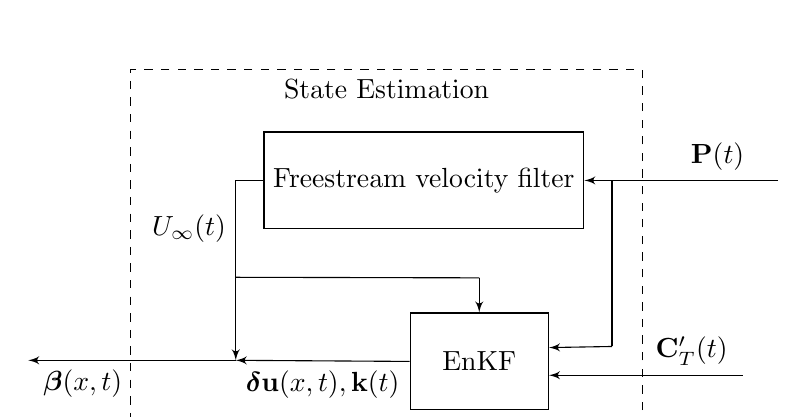
\begin{tikzpicture}[auto, node distance=2.25cm,>=latex']

% Blocks and Nodes
\node [block, name=FVF] {Freestream velocity filter};
\node [block, below=3em of FVF,xshift=2em] (enkf) {EnKF};
\node [dblock, yshift=-2.5em, xshift=-1.35em, minimum width=18.5em, minimum height=13em, label={[yshift=-1.4em]north:State Estimation}] (dummy) {};
\node [io, right=7em of FVF.east] (P){};
\node [io, right=1em of FVF.east] (P1){};
\node [io, below=6em of P1] (P2){};
\node [io, left=1em of FVF.west] (Ui){};
\node [io, below=3.5em of Ui] (Ui2){};
\node [io, above=1.25em of enkf.north] (Ui3){};
%\node [io, below=2em of Ui3] (Ui4){};
\node [io, below=6.5em of Ui] (out){};
\node [io, left=7.5em of out] (out2){};
\node [io, right=7em of enkf.east, yshift = -0.5em] (Ctp) {};

% Input to output
\draw [->, above right] (P) -- node {$\mathbf{P}(t)$} (FVF.east) {};
\draw [-] (P1) -- node {} (P2) {};
\draw [->] (P2) -- node {} ([yshift=0.5em]enkf.east) {};
\draw [-] (FVF.west) -- node {} (Ui) {};
\draw [-, left] (Ui) -- node {$U_\infty(t)$} (Ui2) {};
\draw [->] (Ui2) -- node {} (out) {};
\draw[-](Ui2) -- node{} (Ui3) {};
\draw[->](Ui3) -- node{} (enkf.north) {};
\draw[->, below left](out) -- node{$\boldsymbol \beta(x,t)$} (out2) {};
\draw[->, above right] (Ctp) -- node{$\mathbf{C}_T'(t)$} ([yshift=-0.5em]enkf.east) {};

%\draw [-] (Ui2) -- node {} (Ui3) {};
%\draw [-] (Ui3) -- node {} (Ui4) {};
%\draw [->] (Ui4) -- node {} ([yshift=1em]enkf.west) {};
\draw [->] (enkf.west) -- node {$\boldsymbol \delta \mathbf{u}(x,t), \mathbf{k}(t)$} (out) {};
\end{tikzpicture}
\end{center}
\caption{\label{fig:est}State estimation block diagram showing ensemble Kalman filter and freestream velocity filter.}
\end{figure}

This approach makes assumptions about the time scales associated with the wake model states and parameters. Since the freestream velocity $U_\infty(t)$ uniformly affects all turbines within the farm, we assume that it represents mesoscale phenomena that change over relatively long time scales compared to the advective scale of the wind farm. In other words, the incoming wind speed changes more slowly than the travel time of the wind through the farm. As a result, the slowly-varying freestream velocity is estimated using a first-order relaxation of measurements of the power at the first row of turbines turbine $P_1(t)$ with a time constant $\tau$
\begin{equation}
\tau \frac{dU_\infty}{dt} =  \frac{4+C_{T1}'(t)}{4} \left( \frac{8P_1(t)}{M \rho \pi D^2C_{T1}'(t)} \right)^\frac{1}{3} - U_\infty(t). \! 
\end{equation}

Since the wake expansion parameters $k_n(t)$ and velocity deficits $\delta u_n(x,t)$ vary over shorter time scales, and are therefore estimated using an EnKF~\cite{Evensen2003a} in the following manner. We first reformulate the continuous problem as a discrete update equation and select a noise model to approximate modeling errors. For simplicity, we consider an explicit first-order temporal and spatial discretization of the wake model with $N_x$ grid points in the streamwise direction. Using this discretization, the EnKF states---composed of discretizations of the velocity deficit fields $\boldsymbol \delta \mathbf{u}(x)$ and the wake expansion coefficient vector $\mathbf{k}(t)$---become the following finite-dimensional column vector
\begin{equation}
\boldsymbol \psi = \left[ \boldsymbol \delta \mathbf{u_1}^T,\hdots, \boldsymbol \delta \mathbf{u_N}^T, k_1, \hdots, k_N \right]^T \in \mathbb{R}^{N_s}, 
\end{equation}
where each vector $\boldsymbol \delta \mathbf{u_n}$ is a column vector representing the spatial discretization of $\delta u_n(x)$. 
The number of states is $N_s = (N_x+1)N$, where $N$ is the number of turbine rows. Similarly, the column vector consisting of the measured power output of each row of turbines is denoted $\boldsymbol \xi = \mathbf{P}(t) \in \mathbb{R}^{N_m}$. Since one measurement is taken at each turbine row, the number of measurements equals the number of turbine rows, i.e. $N_m = N$.

The resulting modeled wind farm system is governed by the discrete update equations~\eqref{eq:nonlinear_plant1}--\eqref{eq:nonlinear_plant2}, where $\boldsymbol \psi_{k+1} = \mathbf{f}( \boldsymbol \psi_k, \mathbf{C}_{Tk}')$ and $ \boldsymbol \xi_k = \mathbf{h}(\boldsymbol \psi_k, \mathbf{C}_{Tk}')$ are temporal and spatial discretizations of~\eqref{eq:delta_un}--\eqref{eq:forcing} and~\eqref{eq:estimated_velocity}--\eqref{eq:estimated_power_row}, respectively. Measurement and modeling errors are represented by the i.i.d. white noise processes $\boldsymbol \epsilon \in \mathbb{R}^N_m$ and $\boldsymbol \chi \in \mathbb{R}^{N_p}$ with $N_p = 2N$, respectively. All measurement noise has zero mean and equal variance $\sigma_P^2$. The process noise is subdivided into two vectors $\boldsymbol \chi = [\boldsymbol \chi_{\delta u}^T, \boldsymbol \chi_k^T]^T \in \mathbb{R}^{N_p}$, where $\boldsymbol \chi_{\delta u} \in \mathbb{R}^N$ has variance $\sigma_{\delta u}^2$  with zero mean and $\boldsymbol \chi_k \in \mathbb{R}^N$ has variance $\sigma_{k}^2$ with zero mean.

In many applications, independent process noise enters all states, i.e. the identify matrix would be chosen for $\mathbf{J}$. In this application, we wish to only supply one error correction term to each wake deficit equation. Therefore, the error terms have a lower dimension and are distributed to each wake deficit field independently. This distribution is implemented by selecting
\begin{equation}
\mathbf{J} = 
\begin{bmatrix}
\mathbf{J}_{\delta u} & \mathbf{0}_{N_x N\times N}\\
 \mathbf{0}_{N\times N} & \mathbf{I}_{N \times N}
\end{bmatrix}\in \mathbb{R}^{N_s \times 2N},
\end{equation}
where $\mathbf{I}_{N \times N}$ is the identity, $\mathbf{0}$ are appropriately sized matrices filled with zeros, and the matrix $\mathbf{J}_{\delta u}$ distributes the process noise $\boldsymbol \chi_{\delta u}$ to the wake deficits $\boldsymbol \delta \mathbf{u}$. We assume the wake deficit uncertainties are independent, such that $\mathbf{J}_{\delta u}$ is the block diagonal matrix
\begin{equation}
\mathbf{J}_{\delta u} = 
\begin{bmatrix}
\mathbf{G_1} 	& 			 &			&				\\
			& \mathbf{G_2} & 			&				\\
			&			& \ddots 		&				\\
			&			&			& \mathbf{G_N}	
\end{bmatrix}\in \mathbb{R}^{N_x N \times N}
\end{equation}
where each column vector $\mathbf{G_n} \in \mathbb{R}^{Nx}$ is a spatial discretization of $G(x-s_n)$ in~\eqref{eq:gaussian}. The resulting noise is therefore only distributed about each turbine and there is no noise coupling between turbine rows.

\subsection{Validation -- simulations}
\label{subsec:estimation-ensemble-validation}
The state and parameter estimation, discussed in Section~\ref{subsec:estimation-ensemble-wake} of the wake velocity deficits $\delta u_n(x,t)$, wake expansion coefficients $k_n(t)$, and freestream velocity $U_\infty(t)$ is tested using measurements from three LES of an 84-turbine wind farm, discussed in Section~\ref{subsec:methods-les-farm}, with independent initial conditions. For each test, the wake expansion coefficients are all set to the same initial value of $k_n = 0.05$. The standard deviation of the state and output perturbations---$\sigma_k = 0.0001$, $\sigma_{\delta u} = 0.05$ m/s, and $\sigma_P = 0.29$ MW---are tuned to provide good estimation performance. An ensemble of 250 members is generated by forcing with random noise terms. Each noise term is a normally-distributed number proportional to the standard deviation times the square-root of the step size~\cite{Evensen2003a}. The initial error distributions are formed by integrating each member forward in time~\cite{Evensen2003a} for one advective time scale of the entire farm.

\begin{table}[b]
\caption{Average relative estimation error of power $\frac{1}{T}\int_0^T |\hat{P}_n - P_n|/P_n \, dt$ (\%) by row $n$.}
\label{tab:P_error}
\begin{center}
\begin{tabular}{c c c c c c c c}
\hline
n & 1 & 2 & 3 & 4 & 5 & 6 & 7 \\
\hline
Test 1 & 0.26 & 1.23 & 0.39 & 0.46 & 0.37 & 0.33 & 0.41 \\
Test 2 & 0.22 & 0.80 & 0.41 & 0.42 & 0.39 & 0.35 & 0.35 \\
Test 3 & 0.23 & 0.68 & 0.41 & 0.47 & 0.38 & 0.37 & 0.37 \\
\hline
\end{tabular}
\end{center}
\end{table}

\begin{figure}
\centering
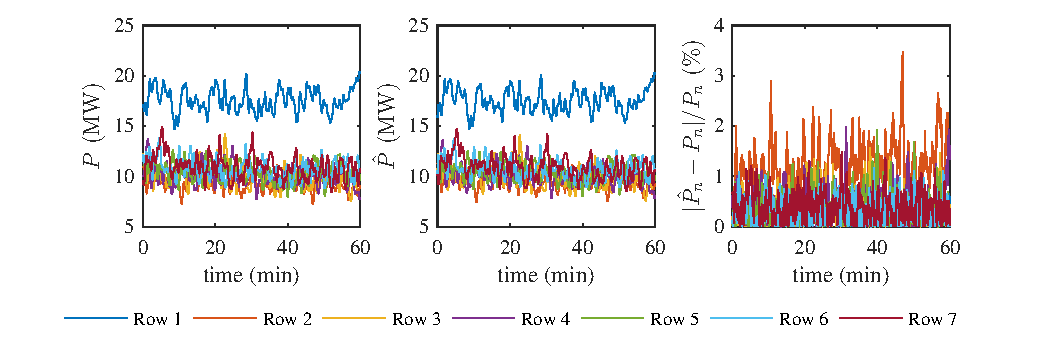
\includegraphics{./fig/r1-power.pdf}
\caption{Power generation of wind farm rows in LES (left) and the EnKF (center), as well as the instantaneous relative error of the wake model estimation for each row (right).}
\label{fig:r1-power}
\end{figure}

To examine the error in power estimation, we use the average relative estimation error measure $\frac{1}{T}\int_0^T |\hat{P}_n(t) - P_n(t)|/P_n(t) \, dt$ for each row, where $P_n(t)$ is the measured power in LES and $\hat{P}_n(t)$ is the estimated power. Table~\ref{tab:P_error} shows the average relative estimation error for all initial conditions. Instantaneous plots of the measured power from LES, the estimated power, and the relative error by row are shown in Figure~\ref{fig:r1-power}. Taken together, these results demonstrate that the instantaneous relative error does not exceed 4\% and the average relative estimation error is always less than 1.25\%.

\begin{figure}
\centering
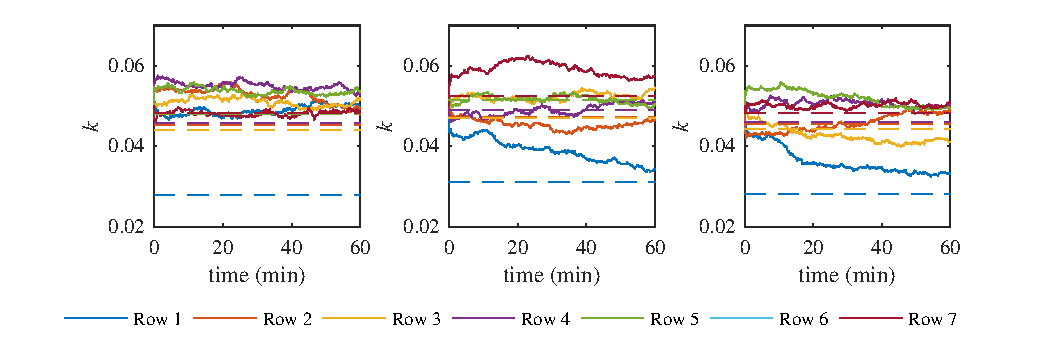
\includegraphics{./fig/k.pdf}
\caption{Comparison of wake expansion coefficients by row as calculated using EnKF (\full) and \textit{ex post facto} best fit of mean power generation using the wake model (\broken). Each panel shows a different initial condition. Two of the three panels capture the substantial difference between the wake expansion rates of the first row and subsequent rows.}
\label{fig:k}
\end{figure}


The estimated values of the wake expansion coefficients are shown in Figure~\ref{fig:k}. For each initial condition, the wake expansion coefficients are compared to a best-fit estimate of these coefficients from the average power of each row over the entire validation window. This best-fit is performed after the simulation and assumes a constant wake expansion rate for each turbine row for the entire window. For each initial condition, these best-fit coefficients demonstrate that the wake expansion rate is lower $k_1 \approx 0.03$ for the first row than subsequent rows $k_n \approx 0.05$. For the last two initial conditions, we see that the estimated wake expansion coefficients approach the distribution of wake expansion coefficients expected from the best fit. The first initial condition, however, does not approach the expected distribution, and more exploration is needed to study this case.


The wake model's streamwise velocity field $u(x,t)$ defined in~\eqref{eq:u} is compared to the LES velocity field $\tilde{u}(x,y,z_h,t)$ at the height of the turbine rotor $z_h$. In order to compare the modeled streamwise velocity along each turbine row, the row-averaged LES velocity field is computed using
\begin{equation}
\label{eq:u_tilde_avg}
\langle \tilde{u} \rangle(x,t) = \frac{1}{DM}\int_0^{L_y} \left[\sum_{m=1}^M H\left(\frac{D}{2}-|y-y_m|\right) \right] \tilde{u}(x,y,z_h,t) \, dy,
\end{equation}
where $H(y)$ is the Heaviside function and $y_m$ is the location of the $m$-th column of turbines. Figure~\ref{fig:u} compares a modeled streamwise velocity field using the EnKF $u(x,t)$ to a row-averaged streamwise velocity profile from LES $\langle \tilde{u} \rangle(x,t)$. This velocity field comparison demonstrates good correspondence between the measured and estimated velocity field near the location of each turbine and captures the changing wake expansion rates and advection of the velocity deficits. As expected, the errors increase downstream of each turbine where measurements are not available.

\begin{figure}[t!]
\centering
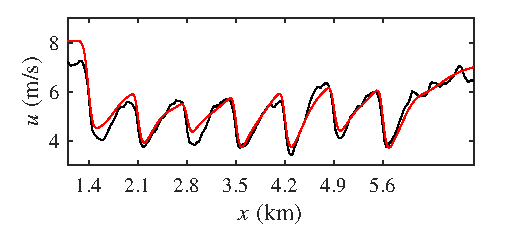
\includegraphics[width=0.65\textwidth]{./fig/u.pdf}
\caption{Instantaneous row-averaged velocity profile from LES (\full), as defined in~\eqref{eq:u_tilde_avg} and the EnKF wake model estimate ({\color{red}\full}), as defined in~\eqref{eq:u} and~\eqref{eq:enkf_final}. Each tick mark denotes a turbine row location.}
\label{fig:u}
\end{figure}

\section{Conclusions}
\label{sec:estimation-conclusons}
Sensing and estimation is vital for providing effective control through closed-loop feedback. In this chapter, we present two methods for providing error correction using measures of power within the wind farm. The first approach is simple to implement, but does not provide state and parameter correction. The second approach uses an EnKF to provide online state and parameter estimation in a computationally efficient manner. The addition of the EnKF provides a more practical approach for estimating wake model parameters and correcting wake model states because parameters do not have to be fit prior to initiation of the control.






\chapter{Model-based receding horizon control}
\label{chap:rhc}
\chaptermark{Model-based receding horizon control}

In this chapter, we address the power tracking problem of secondary frequency regulation using a model-based receding horizon control method~\cite{Rawlings2009a}.  Previous work has used a high-fidelity numerical simulation as a state-space representation of the wind farm for the associated optimal control problem~\cite{Goit2015a}. Instead, we use the time-varying one-dimensional PDE wake model discussed in Section~\ref{sec:dynwake-1d}. Feedback from measurements of wind velocity at each turbine is used to correct modeling errors at each control step. By reducing the number of states by many orders of magnitude, the online optimization problem can be solved in real time. We test the controller on a LES wind farm test system ith actuator disk turbine models, discussed in more detail in Section~\ref{subsec:methods-les-farm}. A diagram of the controlled wind farm system is shown in Figure~\ref{fig:diagram}.

\begin{figure}[]
\centering
\includegraphics[width=\textwidth]{./fig/block_diagram.pdf}
\caption{Diagram of the controlled wind farm system used to track a power reference signal $\text{P}_\text{ref}$. The model-based receding horizon controller (left block) sends local thrust coefficient control signals $\text{C}_\text{T}'$ to the wind farm test system (right block) and closed-loop feedback is based on wind speed measurements $\mathbf{u}$ at each turbine that are passed though an error correction filter. The wind farm is depicted via instantaneous streamwise velocity contours from LES, where slow velocity is blue and high velocity is red. Turbine locations are shown as black lines toward the end of the domain.}
\label{fig:diagram}
\end{figure}

\section{Control design}
\label{sec:rhc-control}

We now incorporate the model developed in Section~\ref{sec:dynwake-1d} into a model-based receding horizon control framework~\cite{Rawlings2009a}. This approach to the power-tracking problem iteratively solves a finite-time optimal control problem, as shown in the schematic diagram of Figure~\ref{fig:receding_horizon}. At each iteration, the problem is solved for a time horizon of length $T$. The controls computed for each iteration, however, are only implemented for a time period of length $T_A < T$, after which the optimal control problem is re-solved~\cite{Bewley2001a, Goit2015a}. Closed-loop error correction is provided using the temporally-damped correction of Section~\ref{sec:estimation-damped}.

The local thrust coefficient $C_T'$ is used as the control variable in the receding horizon control. While generator torque or blade pitch angle are more realistic wind turbine control variables~\cite{Pao2011a}, the local thrust coefficient can parameterize these controls~\cite{Goit2015a}. The local thrust coefficient, however, should be limited to ensure realistic operating conditions. For ease of implementation, we add a regularization term to the cost functional of the optimal control problem described below instead of constraining the optimal control problem using box constraints~\cite{Goit2015a}. 

For each optimization iteration, the power tracking problem can be rewritten as a minimization problem of a cost functional $\mathcal{J}$ constrained by the wake model
\begin{align}
\label{eq:minimize_J}
\underset{\mathbf{C_{T}'}, \mathbf{q}}{\text{minimize}} \qquad & \mathcal{J}(\mathbf{C_T'}, \mathbf{q} ) \\
\label{eq:constraint1}
\text{subject to} \qquad & \frac{\partial \delta u_n}{\partial t} +U_\infty \frac{\partial \delta u_n}{\partial x} = -w_n(x) \delta u_n(x,t) + f_n(x,t) \\
\label{eq:constraint2}
& \hat{u}_n (t) = U_\infty - \int_0^L  \left(\sum_{m=1}^N \delta u_m^2(x,t)\right)^{1/2}G(x - s_n) \, dx + \epsilon_n(t),
\end{align}
where the states are $\mathbf{q} \equiv [\boldsymbol \delta \mathbf{u}(x,t), \mathbf{\hat{u}}(t)]$. We use a cost functional
\begin{equation}
\begin{split}
\mathcal{J} =& \frac{1}{\mathcal{P}^2T}\int_0^T \left( \sum_{n=1}^{N}\hat{P}_n(t)  - P_\text{ref}(t)  \right)^2 \, dt + \frac{\eta}{T}\sum_{n=1}^{N} \int_0^T \left( C_{Tn}'(t)  - C'_{T\text{ref}}\right)^2 \, dt \\
&+ \gamma T\sum_{n=1}^{N} \int_0^T \left( \frac{d C_{Tn}'}{dt}\right)^2 \, dt
\end{split}
\end{equation}
that is the weighted sum of three terms: the first describes the reference tracking goal; the second penalizes deviations away from the pre-control thrust coefficient $C'_{T\text{ref}}$,  which can be seen as a relaxation of bounds on the local thrust coefficient; and the third penalizes large time derivatives of the thrust coefficients to prevent high frequency oscillations in the control. The constant $\mathcal{P} = M \frac{1}{2}\rho\frac{ \pi D^2}{4} U_\infty^3 $ normalizes the power of each row of $M$ turbines and makes the regularization cost functionals the same order of magnitude as the tracking cost functional. The weighting coefficients $\eta$ and $\gamma$, which are much smaller than one, are the relative weights of the regularizations.

\begin{figure}[t]
\centering
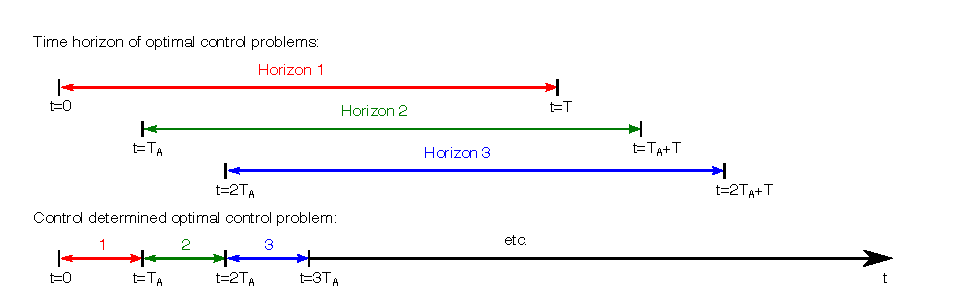
\includegraphics[width=\textwidth]{./fig/receding_horizon.pdf}
\caption{Schematic diagram of the receding horizon control approach.}
\label{fig:receding_horizon}
\end{figure}

We solve the optimization problem by reformulating it using the unconstrained reduced cost functional $\tilde{\mathcal{J}}(\mathbf{C_T'}) = \mathcal{J}(\mathbf{q},\mathbf{C_T'})$~\cite{Bewley2001a, Goit2015a} and minimizing this modified problem in the manner discussed in Section~\ref{sec:methods-pdeopt}. The minimization is performed for a fixed number of iterations using the gradient-based nonlinear Polak-Ribi\`{e}re conjugate gradient method~\cite{Press2007a} combined with the Mor\'{e}-Thuente line search method~\cite{More1994a}. Each Polak-Ribi\`{e}re conjugate gradient iteration requires the computation of the gradient of the reduced cost functional $\nabla\tilde{\mathcal{J}}$ for a given control $\mathbf{C_T'}(t)$. Even for this simplified wake model, direct finite differencing is impractical; instead the gradient is computed using one backward simulation of the adjoint equations, as discussed in Section~\ref{sec:methods-pdeopt}.

The gradient of the reduced cost functional and the adjoint equations are derived using the formal Lagrangian method~\cite{Goit2015a, Borzi2011a}. A Lagrangian is constructed with adjoint variables $\mathbf{q^*} \equiv [\boldsymbol \delta \mathbf{u}^*(x,t), \mathbf{\hat{u}^*}(t)]$ as Lagrange multipliers, which are denoted by stars
\begin{align}
&\mathcal{L}(\mathbf{C_T'}, \mathbf{q}, \mathbf{q^*}) = \mathcal{J}(\mathbf{C_T'},\mathbf{q}) \\
&+ \sum_{n=1}^N \int_0^T \int_0^L \left[   \frac{\partial \delta u_n}{\partial t} + U_\infty \frac{\partial \delta u_n}{\partial x} + w_n(x) \delta u_n(x,t) - f_n(x,t)   \right] \delta u_n^*(x,t) \, dx \, dt    \nonumber\\
&+ \sum_{n=1}^N \int_0^T\left[\hat{u}_n (t) - U_\infty + \int_0^L  \left(\sum_{m=1}^N \delta u_m^2(x,t)\right)^{1/2}G(x - s_n) \, dx - \epsilon_n(t) \right]  \, \hat{u}_n^*(t) \, dt. \nonumber
\end{align}
Let the G\^{a}teaux derivative of a functional $\mathcal{F}(\mathbf{x})$ in the direction $\boldsymbol \Delta x$ be denoted by $\mathcal{F}_\mathbf{x}(\Delta \mathbf{x})$. The adjoint equations are found by enforcing the optimality condition $\mathcal{L}_\mathbf{q}(\Delta \mathbf{q}) = 0$, which after taking the G\^{a}teaux derivative, integrating by parts, and exchanging summation indices can be written as
\begingroup
\allowdisplaybreaks
\begin{align}
& \mathcal{L}_\mathbf{q}(\Delta \mathbf{q})  = \sum_{n=1}^N \int_0^T \int_0^L \left[   \frac{\partial \delta u_n^*}{\partial t} - U_\infty \frac{\partial \delta u_n^*}{\partial x} + w_n(x) \delta u_n^*(x,t) \right.   \nonumber \\
&+ \left. \frac{\sum_{k=1}^N\delta u_n(x,t) \hat{u}_k^*(t) G(x - s_k)  }{\left(\sum_{m=1}^N \delta u_m^2(x,t)\right)^{1/2}}\right] \Delta \delta u_n(x,t) \, dx \, dt  \nonumber\\
&+  \sum_{n=1}^N \int_0^T \left[\frac{\partial \mathcal{J}}{\partial C_{Tn}'} + \hat{u}_n^*(t) \right] \Delta \hat{u}_n(t) \, dt \\
&+ \sum_{n=1}^N \int_0^L U_\infty \left[ \delta u_n^*(x,T) \Delta  \delta u_n(x,T) - \delta u_n^*(x,0) \Delta  \delta u_n(x,0) \right] \, dx \nonumber \\
&+ \sum_{n=1}^N \int_0^T \left[ \delta u_n^*(L,t) \Delta  \delta u_n(L,t) - \delta u_n^*(0,t) \Delta  \delta u_n(0,t) \right] \, dt.  \nonumber
\end{align}
\endgroup
The adjoint equations are found by making each term in square brackets vanish. The gradient of the reduced cost functional is identified in its Reisz representation form
\begin{align}
\label{eq:L_CT}
&\mathcal{L}_\mathbf{C_T'}(\Delta \mathbf{C_T'}) = \sum_{n=1}^N \int_0^T \frac{\partial \tilde{\mathcal{J}}}{\partial C'_{Tn}} \Delta C'_{Tn}(t) \, dt =  \sum_{n=1}^N \int_0^T \frac{\partial \mathcal{J}}{\partial C'_{Tn}} \Delta C'_{Tn}(t) \, dt \nonumber\\
&+ \sum_{n=1}^N \int_0^T \int_0^L - \frac{2 U_\infty^2}{ d_n^2(x)} \left[\frac{\Delta C_{Tn}'(t)}{4 + C_{Tn}'(t)} - \frac{C_{Tn}'(t)\Delta C_{Tn}'(t)}{(4 + C_{Tn}'(t))^2} \right]G(x-s_n) \delta u_n^*(x,t) \, dx \, dt \nonumber \\
=& \sum_{n=1}^N \int_0^T \left[ \frac{\partial \mathcal{J}}{\partial C'_{Tn}} - \frac{8 U_\infty^2 }{(4 + C_{Tn}'(t))^2} \int_0^L\frac{G(x-s_n)}{ d_n^2(x)} \delta u_n^*(x,t) \, dx \right]\Delta C'_{Tn}(t) \, dt,
\end{align}
where the gradient is identified as the term inside the square brackets on the last line of~\eqref{eq:L_CT}.

The adjoint equations then are given by
\begin{align}
\label{eq:adjoint1}
& - \frac{\partial \delta u_n^*}{\delta t} - U_\infty \frac{\partial \delta u_n^*}{\partial x} = -w_n(x) \delta u_n^*(x,t) + f_n^*(x,t) \\
\label{eq:adjoint2}
& \hat{u}_n^*(t) = \frac{\partial \mathcal{J}}{\partial C_{Tn}'}
\end{align}
with the final condition $\delta u_n^*(x,T) = 0$ and boundary condition $\delta u_n^*(L,t) = 0$. Note that these equations have specified final values and must be solved backward in time with flow occurring from outlet to inlet. Furthermore, the adjoint of the local turbine velocities $\hat{u}_n^*(t)$ is computed from the derivative of the cost functional with respect to the control variables. Finally, the adjoint forcing term is a sum of upstream Gaussians
\begin{equation}
f^*_n(x,t) = - \frac{\sum_{k=1}^N G(x-s_k)\hat{u}_k^*(t)}{\sqrt{\sum_{m=1}^N \delta u_m^2(x,t)}}\delta u_n(x,t),
\end{equation} 
and the gradient of the reduced cost functional is
\begin{equation}
\frac{\partial \tilde{\mathcal{J}}}{\partial C_{Tn}'} = \frac{\partial \mathcal{J}}{\partial C_{Tn}'}  - \frac{8 U_\infty^2}{(4 + C_T'(t))^2} \int_0^L \frac{G(x-s_n)}{d_n^2(x)} \delta u_n^*(x,t) \, dx.
\end{equation}
With these analytic formulations, a combination of a forward simulation of the wake model and a backward simulation of the adjoint wake model computes the reduced cost functional and its gradient.

\subsection{Results and discussion}
\label{subsec:rhc-control-results}
The control algorithm is tested using LES of an 84-turbine wind farm as a surrogate for a real wind farm, as discussed in more detail in Section~\ref{subsec:methods-les-farm}. Prior to initiation of the control, the farm is operated at a constant local thrust coefficient $C_{T,\text{ref}}' = 1.33$, which is meant to represent typical wind farm operating conditions~\cite{Calaf2010a}. The five-minute average power output of the farm prior to initiation of the control is used to fit of the wake expansion coefficients and freestream velocity, yielding wake expansion rates of $k_1 = 0.026$--0.028 for the first row and $k_n=0.037$--0.054 for subsequent rows. The freestream velocity $U_\infty$ and wake expansion coefficient are kept constant during the control period. The exponential decay term for the error correction is $\tau = 120$ s. The backward adjoint simulations were integrated using analytically derived discrete adjoints of the forward simulation Runge-Kutta time integration scheme. Third-order downwind biased spatial discretization is used in the adjoint equations. Using this numerical scheme, the gradients computed using the adjoint equations were satisfactorily close to the gradient computed using finite differencing on a small test system with fewer states. 

For the receding horizon control, a control horizon of $T = 40$ min, corresponding to the length of the control simulation, and an advancement time of $T_A = 10$ s are used. Only 100 iterations are used in each optimization iteration to reduce optimization time. The coefficients for the regularizations of the cost function are $\eta = 0.005$ and $\gamma = 2.083\times 10^{-5}$.

\begin{figure}[h]
\begin{center}
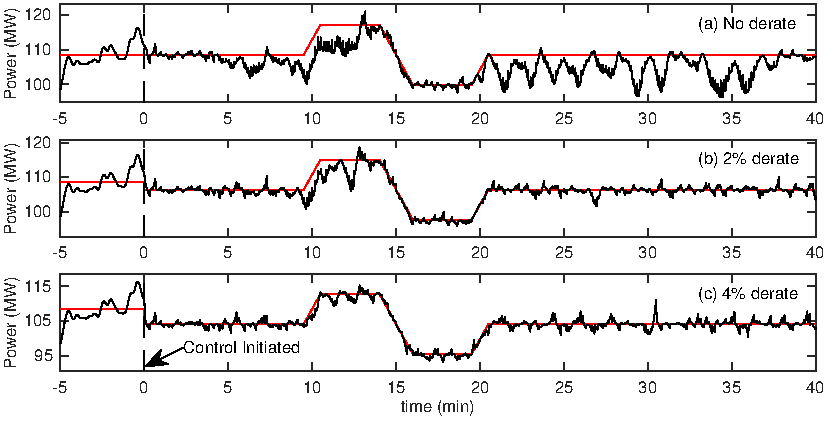
\includegraphics[width=\textwidth]{./fig/Pfarm.pdf}
\caption{Simulated total farm power from controlled LES (black) and reference signal (red) versus time for (a) no derate, (b) 2\% derate, and (c) 4\% derate cases with inflow condition 1. Control is started at t = 0 (denoted by vertical black dashed line), and the pre-control reference signal shows the five-minute pre-control average wind farm power production. Since the magnitude of the reference signal is different in each panel, the bounds of the ordinate are scaled to $P(t) \in [0.95 \min_{0 \le t \le T} P_\text{ref}(t), 1.05\max_{0 \le t \le T}  P_\text{ref}(t)]$.}
\label{fig:Pfarm}
\end{center}
\end{figure}

The power reference signal, shown in red in Figure~\ref{fig:Pfarm}, is specified as 
\begin{equation}
P_\text{ref}(t) = [1-\alpha + r(t) ]P_\text{base}.
\end{equation}
We define the baseline power $P_\text{base}$ as the five-minute average of the power output prior to the initiation of the control. Averaging over five-minute windows was found to provide reasonable averages; for an LES with a constant $C_T' = 1.33$ the root-mean-square of the total power output after averaging over five-minute windows is less than 2.5\% of the mean power output over a 45-minute period. The time-varying change in power setpoint $r(t)$ varies by $\pm 0.08$ and is meant to be representative of secondary frequency regulation signals used by grid operators~\cite{PJMm12}. The parameter $\alpha$ is the reduction in the power setpoints to compensate for the need to track increases in power demand. It is also a measure of the fraction of revenue lost for the supply of bulk power. We consider three different cases $\alpha = 0$, 0.02, and 0.04, which are referred to as derate cases because they correspond to derating the total power output by 0, 2, and 4\% for a given condition. These derates are not imposed by an \textit{a priori} reduction in the local thrust coefficient; instead, the controller imposes the derates by dynamically responding to the power reference signal at the initiation of the control. Each derate case is tested with three inflow initial conditions generated by separate atmospheric boundary layer simulations, resulting in nine total simulations of the control approach in LES.

Table~\ref{tab:rmse} compares the controller performance for the three derate cases under all three inflow conditions. For each inflow condition the baseline five-minute pre-control average power $P_\text{base}$ is provided. The error between the controlled LES wind farm power $P(t)$ and the reference signal $P_\text{ref}(t)$ is reported as the root mean square error 
\begin{equation}
\text{RMSE} = \left(\frac{1}{T} \int_0^T [P(t) - P_\text{ref}(t)]^2 \, dt\,\right)^{1/2}
\end{equation}
 in MW. To compare the performance between different inflow conditions, the RMSE normalized by the baseline power $\text{NRMSE} = \text{RMSE}/P_\text{base}$ is also provided. These results demonstrate that the RMSE decreases with increasing derate, indicating improved performance. Performance can also vary substantially depending on the inflow conditions, but this sensitivity decreases with increasing derate. 
 
\begin{table}
\caption{Comparison of controller performance for three derate cases and three inflow conditions. For each inflow condition the table reports the pre-control five-minute average power $\text{P}_\text{base}$. The error between the controlled LES wind farm power and the reference signal is reported as both the root mean square error (RMSE) in MW and normalized root mean square error (NRMSE) in \% relative to $\text{P}_\text{base}$ in MW.}
\label{tab:rmse}
\centering
\small
\begin{tabular}{c c c c c c c c}
\toprule
Inflow & & \multicolumn{2}{c}{No Derate} & \multicolumn{2}{c}{2\% Derate} & \multicolumn{2}{c}{4\% Derate} \\
Conditions & $P_{\text{base}}$  & RMSE  & NRMSE & RMSE & NRMSE & RMSE & NRMSE  \\
\midrule
1 & 108.6 & 4.30 & 3.96 & 1.63 & 1.50 & 1.07 & 0.98 \\
2 & 96.6 & 1.68 & 1.74 & 0.89 & 0.93 & 0.90 & 0.93 \\
3 & 99.2 & 1.05 & 1.05 & 0.90 & 0.90 & 0.89 & 0.90 \\
\midrule
Mean & & 2.34 & 2.25 & 1.14 & 1.11 & 0.95 & 0.94 \\
\bottomrule
\end{tabular}
\end{table}

Figure~\ref{fig:Pfarm} further illustrates the improved performance of the controller with increasing derate by comparing the total farm power from controlled LES for each case to the reference signal for the first inflow condition. This inflow case has the highest RMSE for all derate cases and thus illustrates the worst performance of the controller for each derate case. For the least successful simulation, the no derate case in Figure~\ref{fig:Pfarm}(a), the control has difficulty following the reference signal. For the 2\% derate case in Figure~\ref{fig:Pfarm}(b) the wind farm power generally follows the reference signal, except when the reference signal requires a large increase in power. For the 4\% derate case shown in Figure~\ref{fig:Pfarm}(c) the total farm power closely follows the reference signal with fluctuations about the reference. Interestingly, the mean power production during minutes 20--40 in the no derate case is lower than the other cases. This may be because the controller has extracted more kinetic energy from the flow field to try to meet the reference signal during the preceding 20 minutes and therefore cannot increase the power level further. Furthermore, the fluctuations during the controlled period are noticeably smaller than the pre-control fluctuations with constant $C_T'$. In other words, the control also damps the natural turbulent fluctuations in power output, which may also be beneficial for system operations.


These results demonstrate the importance of derating the power production in order to provide secondary frequency regulation. Since the power production will naturally fluctuate around an average production level, controlling power at the average may not be possible. For example, the controller is unable to maintain the baseline power during the last half of the control period in the no derate case shown in Figure~\ref{fig:Pfarm}(a). During periods where the reference signal is larger than the available energy from the inflow conditions the control will fail to track the power reference signal. This could also explain the failure to track the signal during the up-ramps in Figure~\ref{fig:Pfarm}(a)--(b), 

The importance of including aerodynamic interactions in the control strategy is highlighted by Figure~\ref{fig:Ctp}, which shows representative control trajectories in each row for inflow condition 3 with no initial derate. In particular, these results show that the control signal for the last row of farm, which does not influence the power output of upstream turbines, operates differently than the other rows. Furthermore, during the few minutes preceding the up-ramp of the reference signal, the thrust coefficients of the first six rows decline in order to move power generation from the first row to downstream rows, as shown in Figure~\ref{fig:P_contribution}. This movement towards a different operating state may allow the farm to extract additional power over a short period (10--15 minutes) by the slow ramping of the thrust coefficients. 

\begin{figure}[h]
\begin{center}
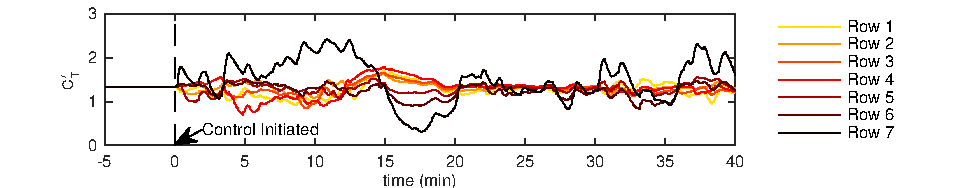
\includegraphics[width=\textwidth]{./fig/Ctp.pdf}
\caption{Control trajectories $\text{C}'_\text{T}$ of each row for inflow condition 3 and no initial derate.}
\label{fig:Ctp}
\end{center}
\end{figure}

\begin{figure}[b]
\begin{center}
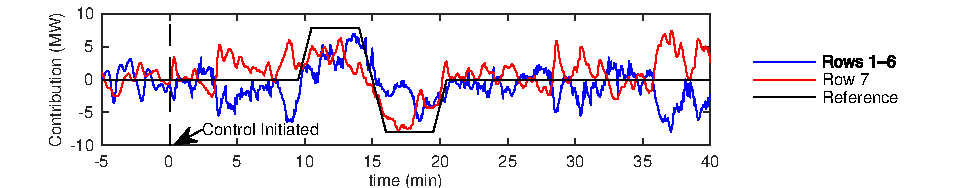
\includegraphics[width=\textwidth]{./fig/Pcont.pdf}
\caption{Contribution of first six rows and last row to the regulation for inflow condition 3 with no initial derate. The contribution is computed by subtracting the pre-control average power production for each collection of rows. The pre-control average power production for the entire farm is subtracted from the reference shown.}
\label{fig:P_contribution}
\end{center}
\end{figure}

By leveraging these aerodynamic effects, the proposed control strategy has demonstrated the potential to reduce the setpoint reduction used in previous work~\cite{Aho2013a, Aho2014a, Jeong2014a}, where the power production is derated by an amount equal to the maximum up-regulation of the signal. The consistent success of the 4\% derate case, indicates that for the test system and initial operating conditions used (LES with the actuator disk model) the derate can be 50\% of that normally employed in single turbine based control strategies. However, the required derate most likely depends on the maximum duration of the required up-regulation, the size of the wind farm, the wind farm spacing and configuration, and the thrust and power coefficient curves of the wind turbines, among other factors. Understanding these effects as well as others affection implementation are a direction for future work.

The reduced derate required to provide this power tracking service has large potential economic consequences for wind operators. Previous studies have indicated that the trade-off between payments from bulk power supply and participation in frequency regulation markets are important for the viability of wind farms participating in frequency regulation. Within the context of previous work, where wind farms were derated by an amount equal to the maximum up-regulation of the signal, the economic viability of wind farm secondary frequency regulation was of some debate~\cite{Kirby2010a, Rose2014a}. Reducing the required derate increases steady-state operating power generation, thereby allowing wind farm operators to provide a higher level of bulk power and still participate in frequency regulation markets; i.e. it reduces the cost burden of providing frequency regulation and may lead to increases in revenue due to the ability to provide this new service.

\section{Grid operator qualification tests}
\label{sec:rhc-pjm}
In this section, we evaluate the control approach described above with regulation test signals from PJM, an independent system operator (ISO) in the United States Eastern Interconnection~\cite{PJMm11, PJMm12}. PJM has two types of secondary frequency regulation signals that are based on the Area Control Error (ACE) signal, a combined measure of the power imbalance and deviation of the frequency from its nominal operating value. The ``RegA'' signal is a low pass filter of the ACE that is generally followed using traditional regulating resources, such as fossil fuel plants. The ``RegD'' signal is a high pass filter of the ACE that can be followed by more quickly responding resources, such as energy storage devices. We evaluate the performance of the controller using PJM's performance evaluation criteria~\cite{PJMm11, PJMm12} to determine whether the controlled wind farm system can meet PJM's threshold for qualification in these two regulation markets. These computations also allow us to evaluate whether wind farms with this control strategy are better suited to provide traditional or fast-acting regulation.

In order to participate in PJM's regulation market, power plants must pass the Regulation Qualification Tests for the particular regulation signal being supplied. These tests are carried out over a 40-minute period, and the tracking capability is quantified using a composite performance score, which is the weighted sum of accuracy, delay, and precision scores~\cite{PJMm11,PJMm12}. The accuracy score measures the ability of the signal to respond to a change in the ISO regulation signal. The delay score measures the delay in the plant's response to the regulation signal. The precision score measures the difference between the requested power and the plant's power output. A minimum composite score of 75\% is needed to qualify to participate in each of the two regulation services. Once qualified for a particular service, a plant is continuously evaluated; if its average score over the last 100 hours drops below 40\%, then the plant is disqualified from providing the service and must retake the initial performance tests to requalify. 

The performance of the controlled wind farms is evaluated using PJM's published RegA and RegD test signals as well as historical RegA and RegD signals from three hours in 2015~\cite{PJMm11,PJMm12, PJM2018a}. For each regulation signal, we use three different initial conditions for the wind farm and two levels of power derate. As in the previous section, the reference signal for each test is defined as $P_\text{ref}(t) = [1 - \alpha + 0.08r(t)]P_\text{base}$, where $P_\text{base}$ is the 5-minute average power prior to initiation of the control, $\alpha$ is the derate amount, and $r(t) \in [-1,1]$ is the regulation signal from the ISO. 

The combination of test signals and initial conditions lead to 48 unique test cases, each of which is given a unique identifier that is a combination of identifiers for each of the variable types shown in Table~\ref{tab:cases}. ``Signal'' refers to the regulation signal type (RegA or RegD), ``Derate'' refers the to derate amount (4 or 6\%), ``Initial condition'' refers to the initial condition of the controlled plant simulation, and ``Period'' refers to the regulation signal period, which is either the PJM test signals or one of the selected hours in 2015. For example, the test case ``RegA.D4.IC1.TS'' refers to the case with the RegA test signal, 4\% derate, and the first initial condition. 
%
\begin{center}
\begin{table}[t]
\caption{\label{tab:cases} Test case identifiers describing the signal type, derate amount, initial condition of the wind farm, and regulation signal period. For example, the test case ``RegD.D6.IC1.H2' refers to the case with the second RegD historical signal, 6\% derate, and the first initial condition.}
\centering
\begin{tabular}{@{}*{7}{l}}
\hline
Identifier & Type & Description\\
\hline
RegA & Signal & Traditional RegA regulation signal\\
RegD & Signal & Fast-responding RegD regulation signal\\
D4 & Derate & Power setpoint is reduced by 4\% of $P_\text{base}$\\
D6 & Derate & Power setpoint is reduced by 6\% of $P_\text{base}$\\
IC1 & Initial condition & Initial condition 1\\
IC2 & Initial condition & Initial condition 2\\
IC3 & Initial condition & Initial condition 3\\
TS & Period & PJM test signals\\
H1 & Period & PJM historical hour 1\\
H2 & Period & PJM historical hour 2\\
H3 & Period & PJM historical hour 3\\
\hline
\end{tabular}
\end{table}
\end{center}

\subsection{Historical PJM regulation signals}
\label{subsec:rhc-pjm-hist}
The number of historical hours used to test the controlled wind farm is constrained by the computational cost of running the model wind farm LES. As a result, it is impractical to select enough hours to sample the entire range of possible regulation signals provided by PJM. To prevent systematic bias, the three hours were selected without considering the characteristics of the regulation signals during those periods. 


\begin{figure}[t]
\begin{center}
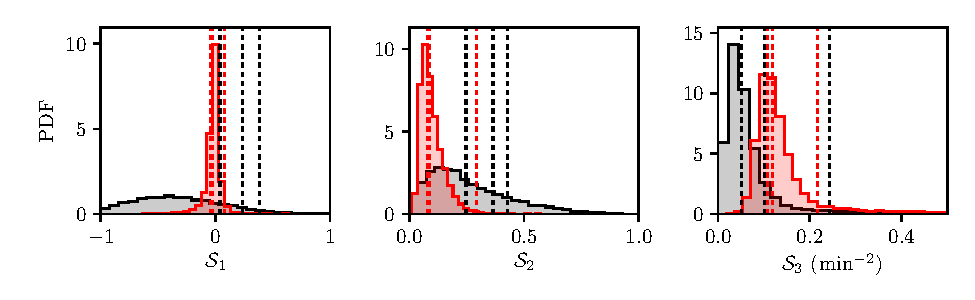
\includegraphics[width=\textwidth]{./fig/f4.pdf}
\end{center}
\caption{\label{fig:pdfs} Probability density functions of $\mathcal{S}_1$--$\mathcal{S}_3$ defined in Eq.~\eqref{eq:stats} for RegA (black) and RegD (red) during 2015. The three selected historical hours are shown in the PDFs as vertical dashed lines.}
\end{figure}

In order to evaluate whether the selected signals are representative cases, we compare them to the range of all possible regulation signals provided by PJM in 2015 using three statistics
\begin{equation}
\label{eq:stats}
\mathcal{S}_1 = \frac{1}{T}\int_0^T r(t) \, dt \qquad \mathcal{S}_2 = \frac{1}{T}\int_0^T r^2(t) \, dt - \mathcal{S}_1^2  \qquad \mathcal{S}_3 = \frac{1}{T}\int_0^T \left(\frac{dr}{dt}\right)^2 \, dt ,
\end{equation}
where $r(t)$ is the regulation signal, $T = 60$ min, $\mathcal{S}_1$ is the mean of $r(t)$, $\mathcal{S}_2$ is the variance of $r(t)$, and $\mathcal{S}_3$ is the variance of $\frac{dr}{dt}$. For each of these statistical measures, the probability density function (PDF) is calculated using all possible hourly signals provided by PJM in 2015 and is shown in Figure~\ref{fig:pdfs}. These PDFs demonstrate the differences between the RegA and RegD signals. The RegA signals have a larger mean and variance than the RegD signals, but the variance of $\frac{dr}{dt}$ is smaller. The values of these statistics for the three selected hours is compared to the PDFs over the entire year in Figure~\ref{fig:pdfs}. These figures show that the selected historical signals represent a reasonable cross section of the possible PJM regulation signals. The only exception, the high percentile ranking in $\mathcal{S}_1$ of the RegA signals, represents a more difficult test for the controlled wind farm because more energy is requested than the average.


\subsection{Wind farm initial conditions}
\label{subsec:rhc-pjm-ic}
We set the initial conditions of the controlled wind farm simulations to correspond to uncontrolled simulations with a local thrust coefficient of $C_{T,\text{ref}}'=1.33$, as previously discussed. The inflow characteristics for the three initial conditions of interest are provided in Table~\ref{tab:params}. The inflow velocities of the initial conditions have a mean $\overline{u} \approx 9.5$ m/s and a standard deviation $\sigma_u \approx 1$ m/s as measured at the first row of turbines during the $T_0 = 5$ min prior to initiation of the control
\begin{align}
\overline{u} &= \frac{4 + C_{T,\text{ref}}'}{4}\frac{1}{T_0 M} \int_{-T_0}^0 \sum_{m=1}^M u_{1m}(t) \, dt \\
\sigma_u &= \frac{4 + C_{T,\text{ref}}'}{4} \left[\frac{1}{T_0M} \int_{-T_0}^0\sum_{m=1}^M \left(u_{1m}(t) - \overline{u}\right)^2 \, dt \right]^{1/2}.
\end{align}
The turbulence intensity as measured at the center of each of the turbine rotors is approximately 13\%, which corresponds to low to medium IEC turbulence levels~\cite{IEC2005a}. The simulations assume region 2 operation~\cite{Johnson2006a} with idealized aerodynamic characteristics of $C_P' = C_T'$. In order to avoid any significant interaction with the rated regime, we presume wind turbines with a rated wind speed of at least 12m/s, which corresponds to the 99th percentile of the LES velocity field.

The required parameters of the static and dynamic wake models, inlet velocity $U_\infty$ and wake expansion coefficients $k_n$, are also calculated for each initial condition using measurements from the $T_0 = 5$ min prior to initialization of the control. The inlet velocity is set using the relationship $U_\infty =\frac{1}{4}(4 + C_{T,\text{ref}}')T^{-1}\int_{-T_0}^0 u_1(t) \, dt$, and the wake expansion coefficients are found using a least squares fit between the measured power and the power predicted by the static model. Note that the inlet velocity for the model is defined using the average power and therefore  the average inflow velocity is not equal to the inlet velocity for the models $\overline{u} \ne U_\infty$. The resulting parameters are also shown in Table~\ref{tab:params}.
%
\begin{center}
\begin{table}[h!]
\caption{\label{tab:params} Characteristics of the three wind farm initial conditions, including mean inlet velocity $\overline{u}$, standard deviation of inlet velocity $\sigma_u$, and turbulence intensity TI. The corresponding wake model inlet velocity $U_\infty$ and wake expansion coefficients $k_n$ are also shown.}
\centering
\begin{tabular}{@{}*{12}{l}}
\hline
Initial & $\overline{u}$ & $\sigma_u$& TI & $U_\infty$& $k_1$ & $k_2$ & $k_3$ & $k_4$ & $k_5$ & $k_6$ & $k_7$\\
condition & m/s & m/s & \% &  m/s & - & - & - & - & - & - & - \\
\hline
1 & 9.53 & 1.12 & 13.6 & 9.65 & 0.028 & 0.049 & 0.041 & 0.047 & 0.053 & 0.054 & 0.054 \\
2 & 9.22 & 0.97 & 13.3 & 9.32 & 0.026 & 0.046 & 0.043 & 0.047 & 0.054 & 0.052 & 0.052 \\
3 & 9.56 & 0.93 & 12.5 & 9.64 & 0.026 & 0.040 & 0.040 & 0.037 & 0.044 & 0.041 & 0.041 \\
\hline
\end{tabular}
\end{table}
\end{center}

\subsection{Results and discussion}
\label{subsec:rhc-pjm-results}
The time evolution of the total controlled LES wind farm power is compared to the reference signals for initial condition 3 and a 4\% derate in Figure~\ref{fig:pfarm4}, which shows all regulation signals (RegA or RegD) and regulation period combinations. The controlled wind farm power production is also compared to the uncontrolled case, where the wind farm is kept at the constant pre-control thrust coefficient. These results demonstrate the good overall tracking performance of the controlled wind farm, except for a few specific periods of under-performance. Furthermore, the results demonstrate that the dynamic-model based receding horizon control method is able to reduce the natural turbulent fluctuations in the wind farm power production. Indeed, the root-mean-square (RMS) of the controlled wind farm power production about the reference signal is 1.06 MW, which is almost a quarter of the 3.93 MW RMS of uncontrolled power production about the baseline power. 

\begin{figure}[t]
\begin{center}
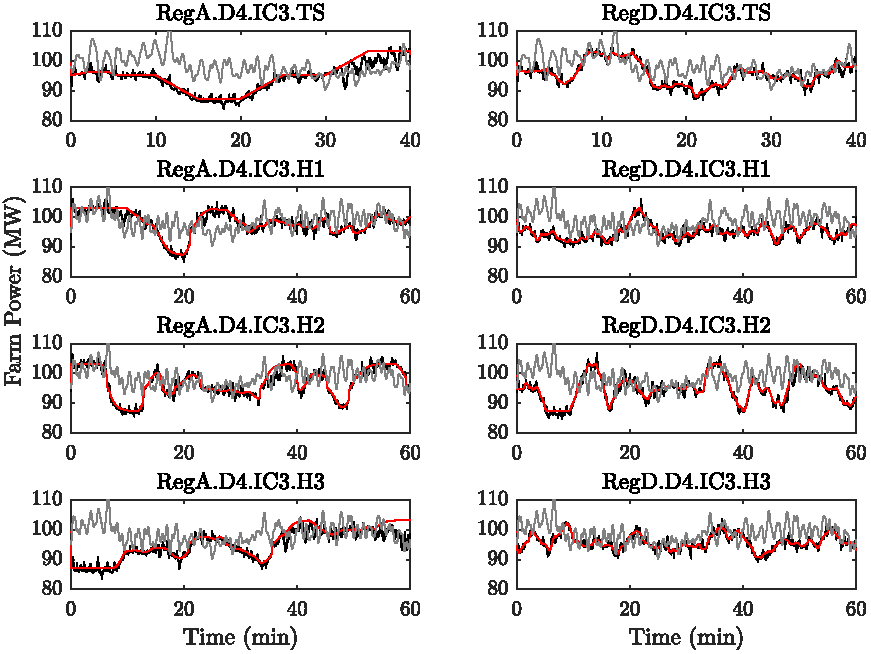
\includegraphics[width=\textwidth]{./fig/f8.pdf}
\end{center}
\caption{\label{fig:pfarm4}Power tracking performance of dynamic-model controlled wind farms comparing simulated farm power from a controlled LES wind farm model (------), an uncontrolled LES wind farm model ({\color{gray}------}), and power reference signals ({\color{red}------}) for 4\% derates and initial condition 3.}
\end{figure}

Quantitative measures of the performance of each regulation signal type (RegA or RegD) for derate values of 4\% and 6\% are shown in terms of PJM's performance scores in Figure~\ref{fig:boxplots}. The controlled wind farm performs better for the RegD signals, meeting the composite score threshold for qualification of 75\% in all cases. The performance of the controlled farm in tracking the RegA signals is also satisfactory for PJM participation, but the controlled farm would not have qualified in all tests. These lower composite scores may be explained by the large values in $\mathcal{S}_1$, which represent the total energy requested in the signals, compared to other PJM signals. However, in cases where the controlled wind farm had poor performance for the RegA signal with 4\% derate, increasing the derate to 6\% markedly improved the overall performance.

\begin{figure}[h]
\begin{center}
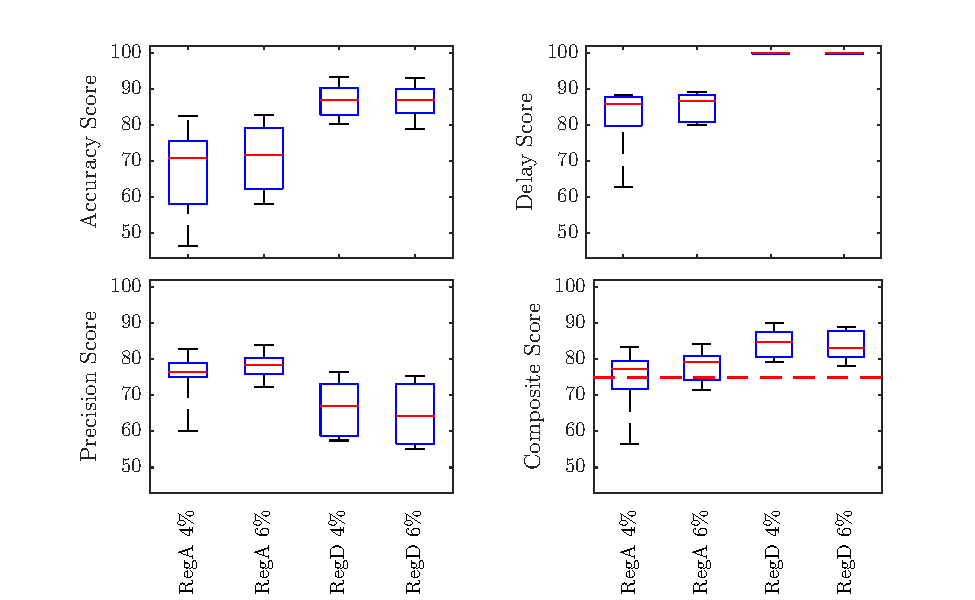
\includegraphics[width=\textwidth]{./fig/f9.pdf}
\end{center}
\caption{\label{fig:boxplots}Boxplots of PJM performance scores for dynamic-model controlled wind farm for all regulation signal types (RegA or RegD) with derate values of 4\% and 6\%. The qualification threshold of 75\% for the composite score ({\color{red}--- --- ---}) is shown in the lower right panel. The average controlled system performance exceeds the 75\% for both signal types, but only the RegD cases pass all of the time.}
\end{figure}

The results shown in Figures~\ref{fig:boxplots}--\ref{fig:reg_a_4d} provide important insights into the possible strengths and limitations of the proposed approach to wind farm control for frequency regulation. These results suggest that wind farms may be well suited to act as a quickly responding resource for grid regulation services. For example, the consistent passing of the composite performance score for the RegD signals indicates that dynamic-model controlled wind farms are able to provide this service reliably. 

The power tracking results in Figure~\ref{fig:pfarm4} demonstrate that the controller is able to track the up-regulation portions of the RegA signals at the beginning of the control period, such as during the first 5--10 minutes of the first two historical signals. In several cases the controlled LES wind farm is able to produce more power than the uncontrolled case, such as after minute 20 of the ``RegA.D4.IC3.H1'' and ``RegD.D4.IC3.H1'' simulations. However, when up-regulation is requested for prolonged periods or towards the end of the control interval, such as the last 10 minutes of the ``RegA.D4.IC3.TS'' and ``RegA.D4.IC3.H3'' cases, the controller does not perform as well. A possible explanation is that the available energy in the wind is slowly changing as the atmospheric boundary layer evolves, as demonstrated by the declining power production of the uncontrolled simulations during these time periods. Since estimates of available energy are readily available over short time horizons, more frequent market clearing may allow wind farms to more effectively provide regulation. Ultimately, future work is needed to determine whether this is a fundamental limitation of the wind farm dynamics or the control strategy and whether additional sensing or forecasting data can overcome these issues.

\section{Comparison to static wake model control}
\label{sec:rhc-static}
In this section we consider the effect of reducing the control design and wake model complexity. In particular, we evaluate the importance of explicitly modeling the dynamics of wake advection by comparing the performance of the dynamic-model approach to a similar static-model approach; i.e. we replace the dynamic wake model with the Jensen model~\cite{Katic1986a}. The standard Jensen model assumes each turbine generates a wake region that expands radially at a linear rate $k$ with increasing downstream distance from the turbine. This leads to following definition of the wake diameter 
\begin{equation}
\label{eq:dw}
D_w(x) = D + 2kx,
\end{equation} 
where $x$ is the streamwise distance from the turbine rotor plane. 

Conservation of mass leads to the following velocity deficit in the wake of the $m$-th turbine in the $n$-th row
\begin{equation}
\label{eq:jens-delta}
\delta u_{nm}(x)  = \frac{2 U_\infty a_{nm}}{\left[D_w(x-s_n)/D\right]^2},
\end{equation}
where $a_{nm}$ is the induction factor and $U_\infty$ is the velocity upstream of the wind farm. This representation yields top-hat profiles of velocity deficits in each cross-stream plane. The velocity field experienced by the each turbine is found by superimposing the squared velocity deficits
\begin{align}
\label{eq:jens-uinfty}
u_{\infty nm} &= U_\infty -\sqrt{ \sum_{(j,k) \in \mathcal{S}_{nm}} \delta u_{jk}^2(s_n-s_j)},
\end{align}
where $\mathcal{S}_{nm}$ is defined as the set of turbines whose wakes lie within the swept area of the turbine rotor of the $m$-th turbine in row $n$. The definition of these sets means that Eq.~\eqref{eq:jens-uinfty} reduces to $u_{\infty1m} = U_\infty$ for the first row of turbines. The power production of each turbine is subsequently found using 
\begin{equation}
\label{eq:Pjens}
\hat{P}_{nm} = \frac{1}{2}\rho\frac{\pi D^2}{4} C_{Pnm} u_{\infty nm}^3,
\end{equation}
where $C_{P nm}$ is the power coefficient of the turbine in row $n$ and column $m$.

To make the Jensen model used here comparable to the dynamic model discussed in Section~\ref{sec:dynwake-1d}, we make the following modifications to the standard Jensen model. First, we consider each row of turbines collectively, which means that each modeled value is homogeneous in the spanwise direction and we neglect the spanwise merging of wakes. To reflect this modification, the column index $m$ used in the Eqs.~\eqref{eq:jens-delta}--\eqref{eq:jens-uinfty} is dropped in subsequent equations. Second, to account for entrance effects in the farm and compensate for the neglected spanwise wake interactions, we allow each wind turbine row to have a separate wake expansion rate $k_n$. 

Furthermore, we express the turbine power production using the local thrust coefficient $C_{Tn}'$ and modeled velocity at the turbine rotor $\hat{u}_n$. From momentum theory, we know that
\begin{equation}
\label{eq:relationships}
a_n = \frac{C_{Tn}'}{4+C_{Tn}'}, \qquad \hat{u}_n = (1-a_n) u_{\infty n}, \quad \text{and}  \qquad  C_{Tn}' = C_{Pn}' = \frac{C_{Tn}}{(1-a_n)^2}.
\end{equation}
Replacing  the induction factor $a_n$ in Eq.~\eqref{eq:jens-delta},  the modeled upstream velocity $u_{\infty n}$ in Eq.~\eqref{eq:jens-uinfty}, and the power power coefficient $C_{Pn}$ in Eq.~\eqref{eq:Pjens} with these equations, the power production can be rewritten as 
\begin{equation}
\label{eq:power-hat}
\hat{P}_{n} = M\frac{1}{2}\rho\frac{\pi D^2}{4} C_{Tn}' \hat{u}_n^3.
\end{equation}

The static wake model used in this work is the Jensen model with the modifications described above. In order to use this static wake model in a model-based controller for the farm power production, the model must be augmented to account for time-varying changes in the local thrust coefficient $C_{Tn}'(t)$. Including time dependency in the thrust coefficient and replacing the induction factor in Eq.~\eqref{eq:jens-delta} with the expression in Eq.~\eqref{eq:relationships} gives the following expression for the velocity deficit for the $n$-th turbine 
\begin{equation}
\label{eq:static1}
\delta u_n(x,t)  = \frac{C_{Tn}'(t)}{4 + C_{Tn}'(t)}\frac{2 U_\infty}{\left[1 + 2k_n (x - s_n)/D\right]^2}.
\end{equation}
With this approach, thrust coefficient changes instantaneously affect the velocity deficit everywhere; i.e., the wakes implicitly have an infinitely fast advection speed. Finally, the velocity at the turbines of the $n$-th row can be found by explicitly writing out the set of upstream turbines in Eq.~\eqref{eq:jens-uinfty} affecting the velocity at the $n$-th turbine and using the equation for the rotor-averaged velocity in Eq.~\eqref{eq:relationships}
\begin{equation}
\label{eq:static2}
\hat{u}_n(t) = \left(1- \frac{C_{Tn}'(t)}{4 + C_{Tn}'(t)}\right)\left( U_\infty - \sqrt{  \sum_{m=1}^{n-1} \delta u_m^2(s_n-s_m) } \, \right).
\end{equation}
Eqs.~\eqref{eq:static1} and~\eqref{eq:static2} are therefore the static wake model equations $\mathbf{W}_s(\mathbf{C}_{T}', \mathbf{q}_s) = \mathbf{0}$, where $\mathbf{q}_s = [\boldsymbol \delta \mathbf{u}, \mathbf{\hat{u}}]$ denote the model states and boldface indicates vectors. 

In order to make appropriate comparisons, the static-model controller solves an online optimization problem with feedback similar to that solved in the dynamic-model controller. As in the dynamic-model controller of Section~\ref{sec:rhc-control}, the static-model controller calculates the local thrust coefficient trajectories by repeatedly solving a minimization problem of the form
\begin{align}
\label{eq:minimize_J_static}
\underset{\mathbf{C_{T}'}, \mathbf{q}}{\text{minimize}} \qquad & \mathcal{J}(\mathbf{C_T'}, \mathbf{q} ) \\
\label{eq:constraint1_static}
\text{subject to} \qquad & \delta u_n(x,t)  = \frac{C_{Tn}'(t)}{4 + C_{Tn}'(t)}\frac{2 U_\infty}{\left[1 + 2k_n (x - s_n)/D\right]^2}\\
\label{eq:constraint2}
& \hat{u}_n(t) = \left(1- \frac{C_{Tn}'(t)}{4 + C_{Tn}'(t)}\right)\left( U_\infty - \sqrt{  \sum_{m=1}^{n-1} \delta u_m^2(s_n-s_m) } \, \right).
\end{align}
where the cost function is
\begin{equation}
\begin{split}
 \mathcal{J}(\mathbf{C_T'}, \mathbf{q} ) =& \frac{1}{\mathcal{P}^2}\left( \sum_{n=1}^N \hat{P}_n(t) - P_{\text{ref}}(t)\right)^2 + \eta \sum_{n=1}^N\left( C_{Tn}'(t) - C_{T, \text{ref}} \right)^2 \\
 &+ \gamma T^2 \sum_{n=1}^N\left( \frac{d C_{Tn}'}{dt}  \right)^2.
 \end{split}
\end{equation}
The constants $\mathcal{P}$, $\gamma$, and $\eta$ are the same as those used in the dynamic-model controller. Although both controllers solve an online optimization problem, the mechanics of the implementation are quite different. Since the equations for the static model have no dynamics, every instance in time is uncoupled. Therefore, the static-model controller can consider each point in time as a separate minimization problem, and the cost functionals can be written solely in terms of the current state. The dynamic-model controller in Section~\ref{sec:rhc-control}, on the other hand, accounts for the time-dependent advection of turbine wake.  Consistent with the distinction between the non-predictive and predictive nature of the static-model and dynamic-model controllers, the functionals for the static wake model are not integrated forward in time. In other words, the static wake model is not a receding horizon method because the modeled system does not include dynamics.

\subsection{Results and discussion}
\label{subsec:rhc-static-results}
The power tracking performance and control trajectories of the controlled wind farm, represented by the LES described in Section~\ref{subsec:methods-les-farm}, are shown in Figures~\ref{fig:reg_a_4d} and~\ref{fig:reg_d_4d}. The left and right panels of these figures show the performance of the static and dynamic-model controllers, respectively. Figure~\ref{fig:reg_a_4d} shows the response of the controlled farms to the RegA test signals, and Figure~\ref{fig:reg_d_4d} shows the response of the controllers to the RegD test signals. The dynamic-model control demonstrates good overall tracking performance, although it has some trouble tracking the reference signal during the last 5--10 minutes of the RegA.D4.IC1.TS and RegA.D4.IC3.TS cases. On the other hand, the static-model control demonstrates poor overall tracking performance, although it is able to track the signal for certain down regulation events, e.g. around minute 20 in all cases in Figure~\ref{fig:reg_a_4d}.

The static-model control method appears to switch between two distinct operating points, depending on the characteristics of the regulation signal. Down-regulation trajectories are often successfully tracked by increasing the thrust coefficient of the first row of turbines to values above \mbox{$C_T'=2$}. This change in operating conditions increases the magnitude of the velocity deficits throughout the farm, thereby reducing the overall wind speed throughout the farm and total power production. When there is a period of up-regulation approaching or the wind farm is slightly underproducing, the controller quickly reduces the upstream thrust coefficients and moves to the Betz-optimal thrust coefficient \mbox{$C_T'=2$} \cite{Goit2015a} for the last row. This operating point is likely the optimal power point for the Jensen model with constant wake expansion coefficients.

\clearpage 

\begin{figure}[h!]
\begin{center}
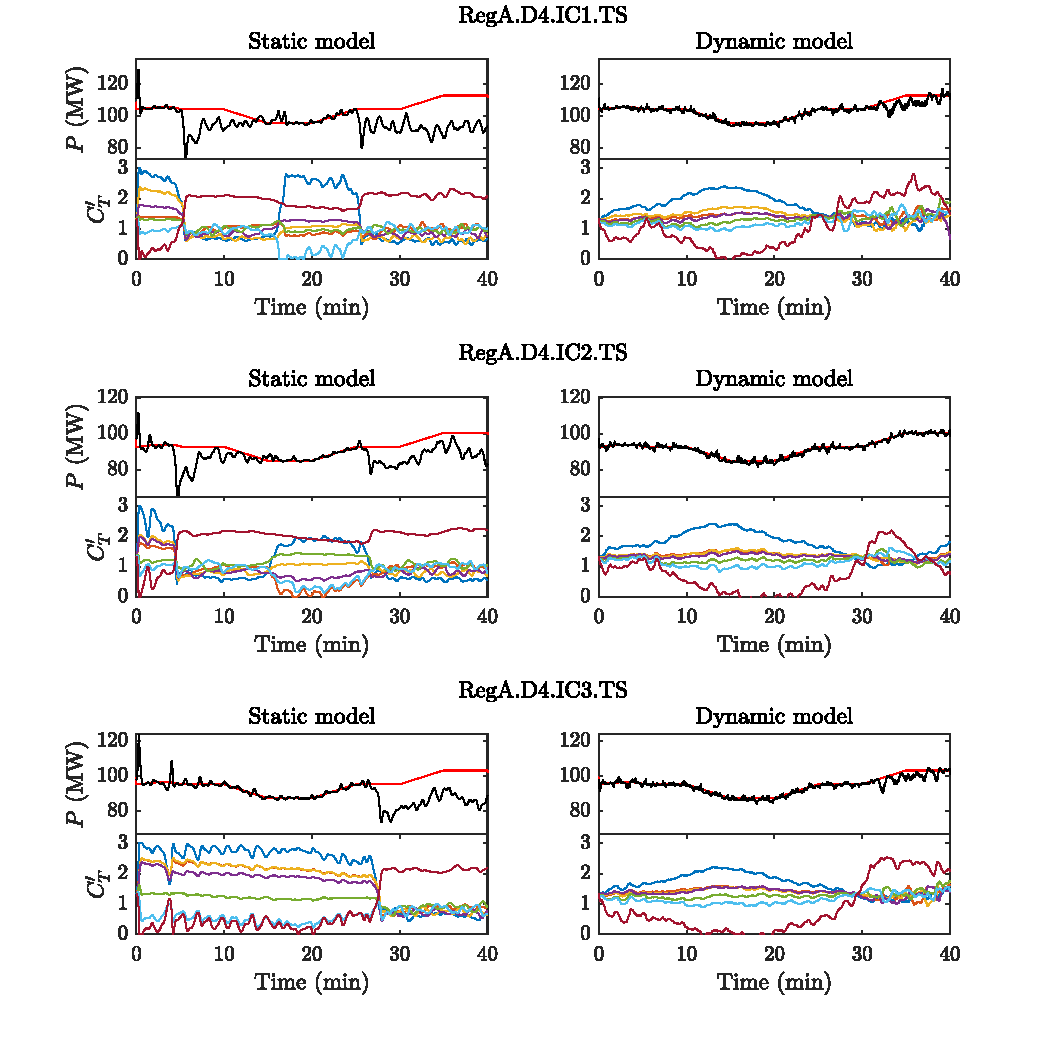
\includegraphics[width=\textwidth]{./fig/f5.pdf}
\end{center}
\caption{\label{fig:reg_a_4d} Comparison of static-model (left) and dynamic-model (right) control methods for RegA test signals with 4\% derates. All three initial conditions 1--3 are shown from top to bottom. The top panel in each row shows the controlled LES wind farm model power production (------) compared to the reference signal ({\color{red}------}). The bottom panel in each row shows the local thrust coefficients calculated by control methods by row: row  1 ({\color{co1}------}), row  2 ({\color{co2}------}), row  3 ({\color{co3}------}), row  4 ({\color{co4}------}), row  5 ({\color{co5}------}), row  6 ({\color{co6}------}), row  7 ({\color{co7}------}).}
\end{figure}

\begin{figure}[h!]
\begin{center}
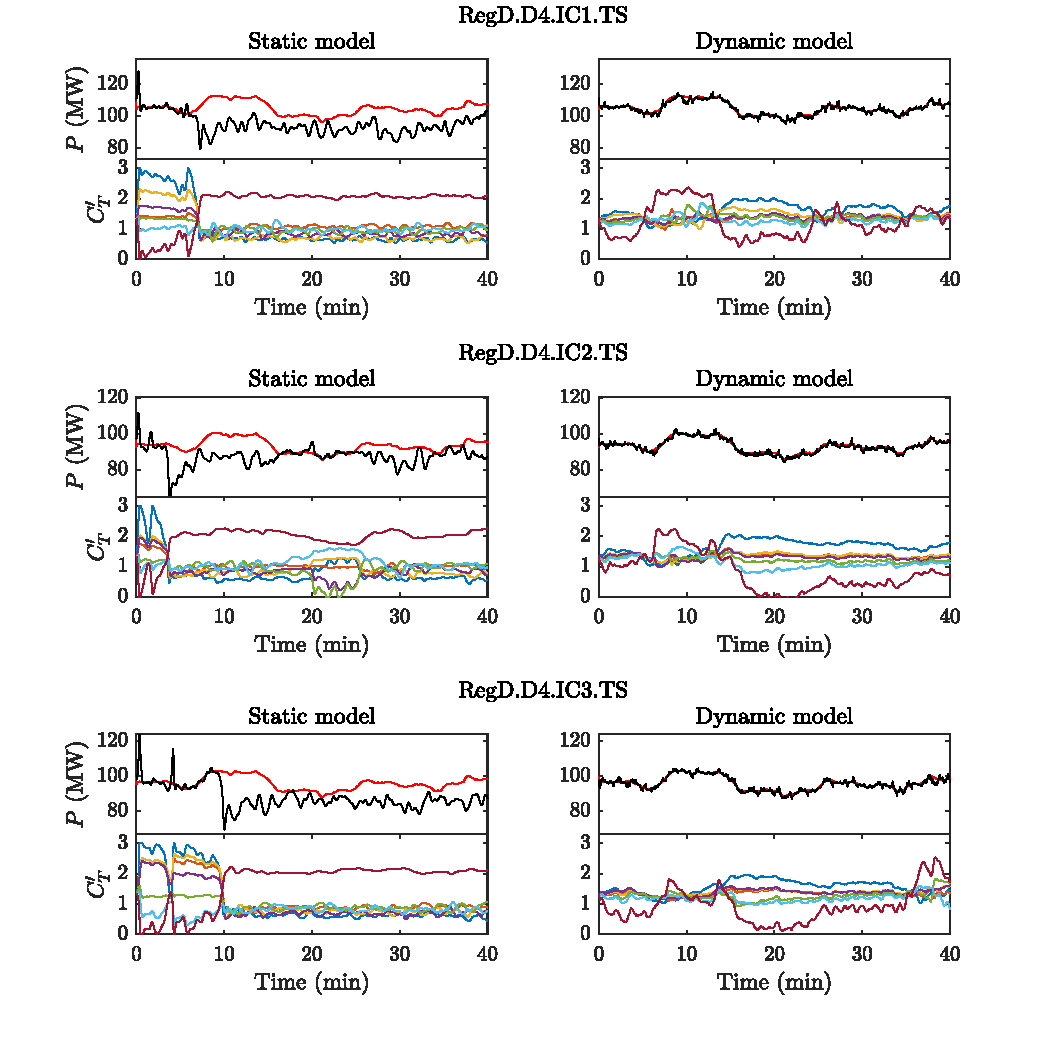
\includegraphics[width=\textwidth]{./fig/f6.pdf}
\end{center}
\caption{\label{fig:reg_d_4d} Comparison of static-model (left) and dynamic-model (right) control methods for RegD test signals with 4\% derates. All three initial conditions 1--3 are shown from top to bottom. The top panel in each row shows the controlled LES wind farm model power production (------) compared to the reference signal ({\color{red}------}). The bottom panel in each row shows the local thrust coefficients calculated by control methods by row: row  1 ({\color{co1}------}), row  2 ({\color{co2}------}), row  3 ({\color{co3}------}), row  4 ({\color{co4}------}), row  5 ({\color{co5}------}), row  6 ({\color{co6}------}), row  7 ({\color{co7}------}).}\end{figure}

\clearpage

\begin{figure}[b!]
\begin{center}
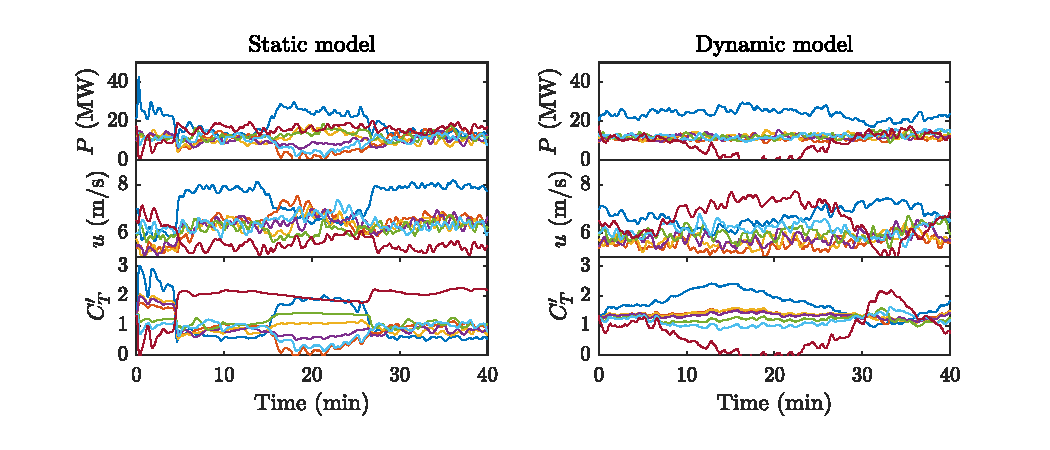
\includegraphics[width=\textwidth]{./fig/f7.pdf}
\end{center}
\caption{\label{fig:reg_a_4d-all} Comparison of static-model (left) and dynamic-model (right) control methods for RegA.D4.IC2.TS simulation case. Each panel shows the controlled LES wind farm model power production, rotor-averaged velocity, and thrust coefficients by row: row  1 ({\color{co1}------}), row  2 ({\color{co2}------}), row  3 ({\color{co3}------}), row  4 ({\color{co4}------}), row  5 ({\color{co5}------}), row  6 ({\color{co6}------}), row  7 ({\color{co7}------}).}\end{figure}

The performance of the static-model control provides an interesting demonstration of the importance of including time dependency in the wake model used in the type of model-based receding horizon control for frequency regulation described in this chapter. In an attempt to track the changing reference signal, the controller switches quickly between the two operating points discussed above. The static Jensen model erroneously models these transitions between operating points as an instantaneous change of the wake velocity deficit throughout the farm. In reality, the air around the turbine will slowly respond to a sudden change in the thrust coefficient and the reduced wake deficit must travel through the farm before the effects of changing upstream thrust coefficients on downstream power production and wind speeds are realized. Detailed trajectories of the power and rotor-averaged velocity of each row in Figure~\ref{fig:reg_a_4d-all}  show that the LES wind farm does not respond instantaneously to the change in operating point. Instead, power production slowly increases between minutes 5 and 15.

As a result of these modeling errors, the static-model controller produces large transient variations in power production when moving between operating points. When moving to the up-regulation operating point identified by the controller, the power production of the farm plunges. In some cases, the total power production slowly recovers to the desired setpoint. Furthermore, all of the static-model control cases in Figures~\ref{fig:reg_a_4d} and~\ref{fig:reg_d_4d} demonstrate significant overshoot in the power production during the first 30 seconds of the simulations as the thrust coefficients quickly move away from the pre-control level. 

The dynamic-model control uses strategies similar to those of the static-model controller, including increasing the thrust coefficient during down-regulation periods and moving toward a Jensen model optimal power point for up-regulation periods. However, by including the time-dependent effects of wake advection, the controller avoids large transient changes when changing between states. The underlying dynamic model can correctly predict the time-varying effect of changing upstream thrust coefficients on downstream power production.

\section{Closed-loop controller with EnKF state and parameter estimation}
\label{sec:rhc-enkf}
In this section we several improvements to the controller introduced in Section~\ref{sec:rhc-control} and implemented in Sections~\ref{subsec:rhc-pjm-hist} and~\ref{subsec:rhc-pjm-ic}. First, we implement the improved state and parameter estimation methods of Section~\ref{subsec:estimation-ensemble-wake}. Second, we eliminate the regulation terms of the cost functional and introduce an auxiliary control variable to keep the control actions within physically acceptable ranges. Finally, we implement a constrained Quasi-Newton optimization method to increase the speed of the control.

In this implementation, we use a cost functional that represents the power tracking problem by penalizing deviations from the reference power $P_\text{ref}(t)$
\begin{equation}
\mathcal{J} = \int_{t_0}^{t_0+T} \left( \sum_{n=1}^N \hat{P}_n(t) - P_\text{ref}(t) \right)^2 \, dt,
\end{equation}
where $t_0$ is the current time. Using this cost function, we solve the following minimization problem
\begin{align}
\label{eq:minimize_J_enkf}
\underset{\boldsymbol \varphi(t), \mathbf{q}(x,t)}{\text{minimize}} \qquad & \mathcal{J}(\mathbf{q}(x,t)) \\
\label{eq:constraint1_enkf}
\text{subject to} \qquad& \mathbf{W}(\mathbf{q}(x,t)) = \mathbf{0} \\
\label{eq:constraint2_enkf}
& \frac{dC_{Tn}'}{dt} = \frac{1}{\tau} \left[ \varphi_n(t) - C_{Tn}'(t)\right]\\
\label{eq:constraint3_enkf}
& 0 \le \varphi_n(t) \le 2.
\end{align}
where $\mathbf{q}(x,t) = [\boldsymbol \delta \mathbf{u}(x,t), \mathbf{\hat{u}}(t), \mathbf{C}_T'(t)]$, $\boldsymbol \varphi(t)$ are auxiliary control variables, and $\mathbf{W}(\mathbf{q}(x,t)) = \mathbf{0}$ represents the wake model discussed of Section~\ref{sec:dynwake-1d}. The auxiliary control variables $\boldsymbol \varphi(t)$, whose rate of change is unconstrained, are used to prevent high-frequency oscillations of the local thrust coefficient. By specifying $\mathbf{C}_T'(t)$ through a  first-order relaxation of $\boldsymbol \varphi(t)$ with a time constant $\tau$, the rate of change of $\mathbf{C}_T'(t)$ is implicitly limited. Furthermore, we select bounds on the control variables of $\varphi_n(t) \in [0, 2]$ to prevent the local thrust coefficient from becoming negative or exceeding the Betz limit of $C_T'=2$~\cite{Meyers2016a}. Minimization is performed using the limited-memory bound-constrained quasi-Newton method L-BFGS-B~\cite{Zhu1997a}. 

With the time horizon and advancement time parameters that are employed in this implementation, as well as the optimization method used, each minimization problem is solved in a fraction of the advancement time on a single processor. In this implementation, we choose a time horizon of $T = 10$ min, which is longer than the time it takes for the wind to travel across the seven-row wind farm considered here, and an advancement time of $T_A \approx 1$ s. This speed is accomplished by using the adjoint equations to compute the gradient, limiting the number of iterations of the minimization algorithm, and using the optimization solution over the previous time horizon as an initial guess for the next time horizon. As a result, this control algorithm can be implemented in real time.

The controlled wind farm is tested in twelve total simulations. We use derates of $\alpha = 0.04$ and 0.06. The signal $r(t)$ is taken from the PJM RegA and RegD test signals~\cite{PJMm11, PJMm12}.  Each derate and signal type combination is tested using all three ending states of the EnKF test cases in Section~\ref{subsec:estimation-ensemble-validation}.

The performance of the controlled wind farm is shown for all twelve simulations in Figure~\ref{fig:enkf-rhc}. Each panel shows the reference signal as described above, the controlled power output, and the uncontrolled power output if the pre-control thrust coefficient $C_{Tn}' = 1.33$ were continued from $t=0$ using the same wind farm state. The performance of the controlled wind farm under the first two initial conditions demonstrate good tracking performance for the the slowly-varying RegA signals as well as the fast-acting RegD signal. The rate-limiting of the control actuation filter results in noticeable fluctuations around the requested power reference signal and some overshoot at the beginning of the control period. However, the controlled farm power has noticeably smaller fluctuations than the turbulent fluctuations of the uncontrolled power. By reducing turbulent fluctuations, the wind farm behaves more like a conventional generator by providing more consistent power output to the grid.


\begin{figure}[h!]
\centering
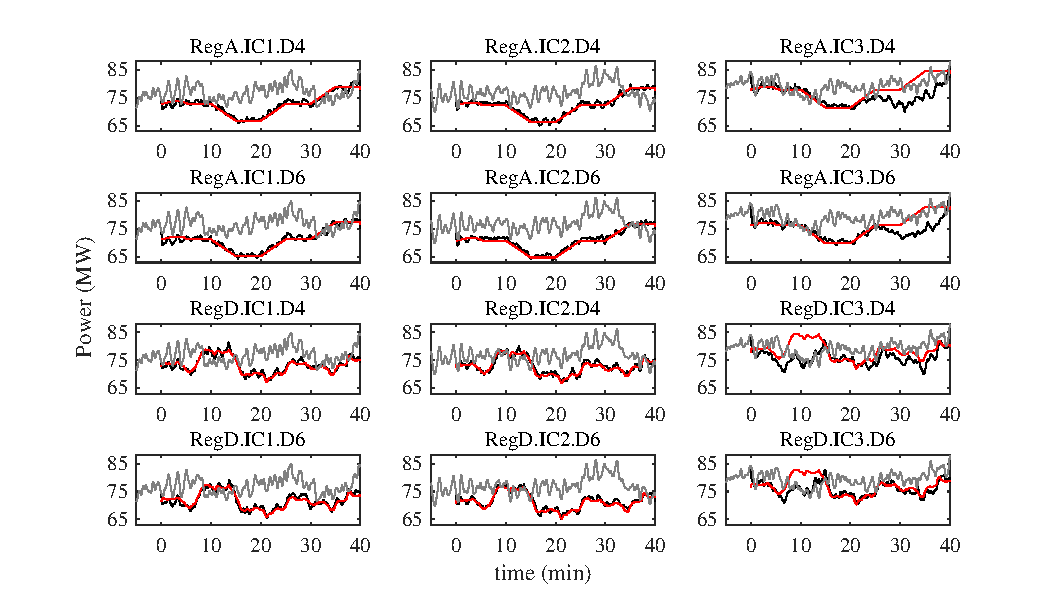
\includegraphics[width=\textwidth]{./fig/enkf-rhc.pdf}
\caption{Controlled wind farm power output (\full) compared to reference signal ({\color{red}\full}) and uncontrolled wind farm power output({\color{gray}\full}). All twelve simulations are shown and denoted by the signal type (RegA or RegD), the initial conditions (IC1--IC3), and derate (D4 for 4\% and D6 for 6\%).}
\label{fig:enkf-rhc}
\end{figure}
These simulations also demonstrate the importance of including a dynamic wake model into the model-based receding horizon control design. During some periods of the simulation---such as around the 10-minute mark of the RegD.IC1.D4 signal and the last 5 minutes of the RegA.IC2.D4 signal---the controlled wind farm was able to produce more power than the uncontrolled farm. Similar trends were seen in Sections~\ref{sec:rhc-control} and~\ref{sec:rhc-static}, where the controller is able to reduce the energy extraction of upstream turbines during periods with more available energy in the flow field, thereby providing increased power production potential for downstream rows. This mechanism would allow for increased production for a short duration by deferring upstream wind turbine energy extraction.

The relatively poor tracking performance of the third initial condition requires further investigation. Periods where the uncontrolled wind farm produces more power than the controlled farm are particularly hard to explain. In some cases, such as the under-production during the last twenty minutes of the RegA cases with the third initial condition, the uncontrolled farm produces more power than requested by the reference signal prior to the period. Therefore, the controlled wind farm probably has at least as much kinetic energy stored in its flow field as the uncontrolled case during this period. Determining the cause of this behavior is the focus of ongoing work.

On the other hand, the under-production around the 10 minute mark of the RegD.IC3.D4 and RegD.IC3.D6 signals in Figure~\ref{fig:enkf-rhc} is likely due to insufficient energy availability. The uncontrolled farm produces less power than requested by the reference signal, and the wind farm may be unable to accommodate the significant increased production requested by the grid operator. In other words, there simply may not be enough available kinetic energy in the flow field to provide the required level of power during this time period.

\section{Conclusions}
In this chapter, we showed that a wind farm using model-based receding horizon controller built around a dynamic wake model (see Section~\ref{sec:dynwake-1d}) can effectively provide secondary frequency regulation for the power grid. The controlled wind farm not only passes numerous qualification tests from PJM, a grid operator in the United States, but can provide secondary frequency regulation with smaller derates than single-turbine controllers. This has important implications for improving the profitability of wind farms providing secondary regulation. This derate reduction is accomplished by leveraging the dynamics of advection and wake dynamics through the wind farm, the controller can store kinetic energy in the flow field for a short period of time. Furthermore, we demonstrated that using a dynamic model is necessary to provide acceptable power tracking by comparing the control method to a similar controller built around the static Jensen model. Finally, we showed how the state and parameter estimation method of Section~\ref{subsec:estimation-ensemble-wake} can be incorporated allow continuous operation of the controller.
\chapter{Coordinated pitch and torque control}
\label{chap:rhc2}
\chaptermark{Coordinated pitch and torque control}

In this chapter, the model-based receding horizon controller proposed and validated in Chapter~\ref{chap:rhc} is extended in three ways. First, the actuation signals are changed to of blade pitch angle and generator torque, which were previously assumed to be parameterized by the thrust coefficient. Second, the wake model, which was previously one dimensional, is extended to two dimensions to  allow for irregular wind farm configurations. Third, the first-order drive train dynamics of the turbines are included to enable the control of rotor speed and storage of kinetic energy in the rotating rotor. While the energy stored in the rotation of the rotor is somewhat less than the energy that can be stored in the flow field (see Appendix~\ref{app}), the rotor's ability to store kinetic energy has been shown to be useful in reducing turbulent power fluctuations in wind farms~\cite{DeRijcke2015a} and providing inertial frequency regulation~\cite{Aho2013a}. The new generalized control framework is easier to implement in existing wind farms because it can be directly tied to existing wind turbine control loops (pitch and generator torque) and improves control authority by allowing direct control of each wind turbine. Numerical simulations illustrate the application of the approach to two wind farm configurations and demonstrate how the kinetic energy reserves are exploited to achieve the tracking objectives.

The remainder of this chapter is organized as follows. Section~\ref{sec:rhc2-model} describes the improved wake model. The controller design is discussed in Section~\ref{sec:rhc2-control}. Simulations are discussed in Section~\ref{sec:rhc2-results}. Conclusions are made in Section~\ref{sec:rhc2-conclusions}.

\section{Wake and turbine model}
\label{sec:rhc2-model}
The time-varying wake and turbine model described in this section are extensions of the model of Section~\ref{sec:dynwake-1d}, which parameterized the turbine actions through the local thrust coefficient $C_T'$ and assumed that each row of turbines operated collectively. The extended model proposed here explicitly includes blade pitch angle $\beta$ and generator torque $Q$. It also incorporates the first-order drive train equations for wind turbines and generalizes the superposition equations to accommodate irregular wind farm configurations.

Consider an $N$-turbine wind farm whose horizontal coordinates parallel and orthogonal to the prevailing wind velocity $U_\infty$ with density $\rho$ are denoted as $x$ and $y$, respectively. Here the wind direction is assumed to remain constant, although future work could extend the model to allow for changing orientations. The corresponding streamwise and lateral spatial extents of the farm are denoted as $L_x$ and $L_y$, respectively. Each turbine has a rotor diameter of $D$ and the $n$-th turbine is located at $(x,y) = (s_n^x,  s_n^y)$. Each turbine rotor has a moment of inertia $J$ and rotates at a speed $\omega_n$. Turbine $n$ is controlled via blade pitch angle $\beta_n$ and generator torque $Q_n$.

The turbines are represented using an actuator disk model, where the control actions of the $n$-th turbine modify the thrust force and aerodynamic power via the thrust $C_{Tn}$ and power $C_{Pn}$ coefficients~\cite{Burton2011a}. These coefficients are assumed to be functions of the pitch angle $\beta_n$ and tip speed ratio $\lambda_n = \frac{\omega_n D}{2 U_\infty}$~\cite{Burton2011a, Pao2011a}. In addition to the local~\cite{Meyers2010a, Calaf2010a} thrust and power coefficients defined in Section~\ref{subsec:methods-les-turbine}, we define the local tip speed ratio as
%
\begin{equation}
\lambda_n' = \frac{\lambda_n}{1-a_n},
\end{equation}
%
where $a_n$ is the induction factor.

The thrust and power coefficient curves are modeled using blade element momentum theory~\cite{Hansen2008a}. Transformed curves based on the local rotor-averaged velocity $C_T'(\beta, \lambda')$ and $C_P'(\beta,\lambda')$  are obtained using interpolation. These relationships are implemented as lookup tables that are interpolated using monotone piecewise cubic interpolation~\cite{Fritsch1980a}.

We use the wake model described in Section~\ref{sec:dynwake-1d} with some modifications to allow for irregular arrangements and pitch and generator torque control. The modifications are highlighted in the following discussion. The forcing function
\begin{equation}
\label{eq:f}
f_n(x,t) = \frac{2 U_\infty^2 }{ d_n^2(x)} \frac{C_{Tn}'(\beta(t), \lambda'(t))}{4 + C_{Tn}'(\beta(t), \lambda'(t))} G(x-s_n)
\end{equation}
is now a function of the pitch angle and tip speed ratio. The velocity field is given by
\begin{equation}
u(x,y,t) = U_\infty - \left( \textstyle{\sum}_{n=1}^N \delta u^2_n(x,t) I_n(x,y) \right)^{1/2},
\end{equation}
where $I_n(x,y)$ is the indicator function specifying the width of the wake  defined by the normalized wake diameter
\begin{equation}
I_n(x,y) = H(d_n(x-s_n^x)D/2 - \vert y-s_n^y \vert),
\end{equation}
and $H(x)$ is the Heaviside (unit step) function. The rotor-averaged velocity at each turbine is subsequently calculated by sampling this velocity field as
\begin{equation}
\hat{u}_n(t) = \int\displaylimits_0^{\vphantom{L_y}L_x} \int\displaylimits_0^{L_y} u(x,y,t) G(x-s^x_n) \tilde{H}(y- s^y_n)\, dy \, dx,
\end{equation}
where $\tilde{H}(y) = D^{-1}H(D/2 - \vert y \vert)$ is a normalized top-hat function. The velocity expression above differ from the model of Section~\ref{sec:dynwake-1d}, which neglected spanwise interactions. The rotational speed $\omega_n(t)$ of the rotor is governed by first order drive-train dynamics~\cite{Pao2011a}
\begin{equation}
\label{eq:rotspeed}
\frac{d \omega_n}{dt} = \frac{1}{J}\left(  \frac{\hat{P}_n(t)}{\omega_n(t)} -Q_n(t) \right),
\end{equation}
where $\hat{P}_n(t) = \frac{1}{8}\rho \pi D^2 C_{Pn}'\hat{u}_n^3(t)$ is the aerodynamic power. The power delivered by the generator to the power grid is 
\begin{equation}
\label{eq:P}
P_n(t) = Q_n(t) \omega_n(t).
\end{equation}
We next present the controller design that uses the wake model described above to calculate control actuation.

\section{Controller design}
\label{sec:rhc2-control}
The control goal in secondary frequency regulation applications is tracking a reference signal $P_\text{ref}(t)$. Here we modify the problem described in Chapter~\ref{chap:rhc} to control the power output of a wind farm, via actuating the blade pitch angles $\beta_n(t)$ and generator torques $Q_n(t)$ of each turbine. The power tracking goal is represented by the cost functional 
\label{sec:controller}
\begin{equation}
\mathcal{J} = \int_{t_0}^{t_0+T} \left( \sum_{n=1}^N Q_n(t) \omega_n(t) - P_\text{ref}(t)\right)^2 \, dt,
\end{equation}
where $Q_n(t) \omega_n(t)$ is the power generated by turbine $n$ and $t_0$ is the current time. The control is then accomplished by solving the following minimization problem
\begin{align}
\label{eq:minimize_J}
\underset{\boldsymbol \varphi(t), \mathbf{q}(x,y,t)}{\text{minimize}} \qquad & \mathcal{J}(\mathbf{q}(x,y,t)) \\
\label{eq:constraint1}
\text{subject to} \qquad& \mathbf{W}(\mathbf{q}(x,y,t), \boldsymbol \varphi(t)) = \mathbf{0} \\
\label{eq:constraint2}
& Q_n(t) = \left(1-\alpha_n(t)\right) \frac{\hat{P}_n(t)}{\omega_n(t)}.
\end{align}
The control inputs $\boldsymbol \varphi(t) = \left[ \boldsymbol \beta_n(t), \boldsymbol \alpha_n(t) \right]$ include the blade pitch angle and an auxiliary control variable $\boldsymbol \alpha(t)$ that specifies the imbalance between the aerodynamic and generator torques; i.e. the torques $\hat{P}_n(t)/\omega_n(t) - Q_n(t) = \alpha_n(t) \hat{P}_n(t)/\omega_n(t)$ are balanced when $\alpha = 0$. This auxiliary control variable increases the computational efficiency of the minimization problem. The states of the wind farm model $\mathbf{q}(x,y,t) = \left[  \boldsymbol \delta \mathbf{u}(x,t), u(x,y,t), \mathbf{\hat{u}}(t), \boldsymbol \omega(t)\right]$ are respectively the wake velocity deficits, superposed velocity field, rotor-averaged velocities, and rotor speeds. The dynamics of the states are governed by the wind farm model \mbox{$\mathbf{W}(\mathbf{q}(x,y,t), \boldsymbol \varphi(t)) = \mathbf{0}$} in~\eqref{eq:f}--\eqref{eq:P}. This wind farm model and generator torque equation~\eqref{eq:constraint2} are represented in discrete-time state space form as
\begin{align}
\mathbf{q}_{k+1} &= \mathbf{f}(\mathbf{q_k}, \boldsymbol \varphi_k)\\
\mathbf{z}_{k} &= \mathbf{h}(\mathbf{q_k}, \boldsymbol \varphi_k).
\end{align}
The nonlinear functions $\mathbf{f}(\mathbf{q_k}, \boldsymbol \varphi_k)$ are first-order temporal and spatial discretizations of~\eqref{eq:f}--\eqref{eq:rotspeed} and~\eqref{eq:constraint2}. The outputs are the power output of each turbine $\mathbf{z}(t) = \mathbf{P}(t)$, and the nonlinear output  equation $\mathbf{h}(\mathbf{q_k}, \boldsymbol \varphi_k)$ corresponds to~\eqref{eq:P}. 

The controller calculates control trajectories for pitch angle and generator torque by solving a reformulation of~\eqref{eq:minimize_J}--\eqref{eq:constraint2} using a receding horizon approach, where $T$ is the length of the time horizon considered. The horizon length is selected to include a significant fraction of the advection time through the farm; i.e. $T \sim L_x/U_\infty$. As previously discussed in Chapter~\ref{chap:rhc}, we solve the PDE-constrained optimization problem~\eqref{eq:minimize_J}--\eqref{eq:constraint2}, via the related unconstrained minimization of the reduced cost functional $\tilde{\mathcal{J}}(\boldsymbol \varphi) = \mathcal{J}(\boldsymbol \varphi, \mathbf{q}(\boldsymbol \varphi))$, where $\mathbf{q}(\boldsymbol \varphi)$ denotes the solution of~\eqref{eq:constraint1}. The reduced cost functional is evaluated by integrating the wind farm model forward in time, and its gradient is evaluated using adjoint equations derived analytically using the formal Lagrangian approach~\cite{Borzi2011a}.  The minimization is performed using a limited-memory bound-constrained quasi-Newton method~\cite{Zhu1997a}. The optimization method is described in detail in Chapter~\ref{chap:rhc}.

The adjoint equations and the gradient of the reduced cost functional are derived using the formal Lagrangian approach~\cite{Borzi2011a},discussed in Section~\ref{sec:methods-pdeopt}. We define the Lagrangian of the PDE-constrained problem by adding the inner product $\langle \cdot, \cdot \rangle$ of the constraining set of equations~\eqref{eq:constraint1}--\eqref{eq:constraint2}, denoted as $\mathbf{B}(\mathbf{q}, \boldsymbol \varphi)$, and a suitable set of Lagrange multipliers \mbox{$\mathbf{q}^* = \left[  \boldsymbol \delta \mathbf{u}^*(x,t), u^*(x,y,t), \mathbf{\hat{u}}^*(t), \boldsymbol \omega^*(t)\right]$} to the cost functional~\eqref{eq:minimize_J} $
\mathcal{L}(\boldsymbol \varphi, \mathbf{q}, \mathbf{q}^*) = \mathcal{J}(\boldsymbol \varphi, \mathbf{q}) + \left\langle \mathbf{B}(\mathbf{q}, \boldsymbol \varphi), \mathbf{q}^*  \right\rangle.$
The adjoint equations $\mathbf{B}^*(\boldsymbol \varphi, \mathbf{q},\mathbf{q}^*)$ are found by representing the Gateaux derivative of the Lagrangian with respect to the state variables in its Riesz representation form \mbox{$\mathcal{L}_\mathbf{q}(\boldsymbol \Delta \mathbf{q}) = \left \langle  \mathbf{B}^*(\boldsymbol \varphi, \mathbf{q},\mathbf{q}^*), \boldsymbol \Delta \mathbf{q} \right\rangle$}. The adjoint equations

\begin{align}
\label{eq:adjoint1}
-\frac{\partial \delta u^*_n}{\delta t} - U_\infty& \frac{\partial \delta u^*_n}{\partial x} =- w_n(x) \delta u^*_n(x,t) + f_n^*(x,t) \\
%
\label{eq:adjoint2}
u^*(x,y,t) =& \sum_{n=1}^N G(x-s_n^x) \frac{I_n(x,y)}{D d_n(x)} \hat{u}_n^*(t)\\
%
\label{eq:adjoint3}
\begin{split}
\hat{u}_n^*(t) =& U_{\mathcal{J}n}(t) + U_{\omega n}(t) \omega_n^*(t) \\
&+ U_{\delta u n}(t) \int_0^{L_x} f_n(x, t) \delta u_n^*(x,t) \, dx
\end{split}\\
%
\label{eq:adjoint4}
\begin{split}
- \frac{d \omega_n^*}{dt} =& W_{\mathcal{J}n}(t) + W_{\omega n}(t) \omega_n^*(t) \\
&+ W_{\delta u n}(t) \int_0^{L_x} f_n(x,t) \delta u_n^*(x,t) \, dx.
\end{split}
 \end{align}
are integrated backward in time with final time boundary conditions. The forcing for the adjoint velocity deficits and the terms on the right hand sides of~\eqref{eq:adjoint3} and~\eqref{eq:adjoint4} are
\begin{equation*}
\begin{split}
f_n^*(x,t) = - \delta u_n&(x,t) \int_0^{L_y} I_n(x,y) u^*(x,y,t)\\
&\left(\sum_{m=1}^N \delta u_m^2(x,t) I_m(x,y)\right)^{-1/2} \, dy 
\end{split}
\end{equation*}
\vspace{-1.4em}
\begin{align*}
\begin{split}
U_{\mathcal{J}n}(t) =& -2 \left(\sum_{m=1}^N \left[ 1 - \alpha_m(t) \right] \hat{P}_m(t) - P_\text{ref}(t)  \right)  \\
&\left[ 1 - \alpha_n(t) \right] \hat{P}_n(t)  \left[ \frac{3}{\hat{u}_n(t)} - \frac{\omega_n(t) R}{C_{Pn}'(t) \hat{u}_n^2(t)} \frac{\partial C_{Pn}'}{\partial \lambda_n'} \right] 
\end{split}\\
%
U_{\omega n}(t) =& \frac{\alpha_n(t)}{J} \hat{P}_n(t) \left[ \frac{3}{\omega_n(t) \hat{u}_n(t)} -  \frac{R}{C_{Pn}'(t) \hat{u}_n^2(t)} \frac{\partial C_{Pn}'}{\partial \lambda_n'} \right] \\
%
U_{\delta u n}(t) =& - \frac{4}{C_{Tn}'(t)}\frac{1}{4 + C_{Tn}'(t)} \frac{\partial C_{Tn}'}{\partial \lambda_n'} \frac{\omega_n(t) R}{\hat{u}_n^2(t)}\\
%
\begin{split}
W_{\mathcal{J}n}(t) = &-2 \left(\sum_{m=1}^N \left[ 1 - \alpha_m(t) \right] \hat{P}_m(t) - P_\text{ref}(t)  \right) \\
 & \left[ 1 - \alpha_n(t) \right] \hat{P}_n(t)\frac{1}{C_{Pn}'(t)} \frac{\partial C_{Pn}'}{\partial \lambda_n'}  \frac{R}{ \hat{u}_n(t)}
\end{split}\\
%
W_{\omega n}(t) =& \frac{\alpha_n(t)}{J} \left[ \frac{\hat{P}_n(t)}{\omega_n(t)} \frac{1}{C_{Pn'}(t)} \frac{\partial C_{Pn}'}{\partial \lambda_n'} \frac{R}{\hat{u}_n(t)} - \frac{\hat{P}_n(t)}{\omega^2_n(t)} \right] \\
%
W_{\delta u n}(t) =&\frac{4}{C_{Tn}'(t)}\frac{1}{4 + C_{Tn}'(t)} \frac{\partial C_{Tn}'}{\partial \lambda_n'} \frac{R}{\hat{u}_n(t)}.
\end{align*}
%

The gradient of the reduced cost functional $\partial \tilde{\mathcal{J}} / \partial \boldsymbol \varphi$ is found by representing the Gateaux derivative of the Lagrangian with respect to the control variables in its Riesz representation form $\mathcal{L}_{\boldsymbol \varphi}(\boldsymbol \Delta {\boldsymbol \varphi}) = \left \langle  \partial \tilde{\mathcal{J}} / \partial \boldsymbol \varphi, \boldsymbol \Delta \boldsymbol \varphi \right\rangle$

%%% alpha gradient %%%
\begin{align}
\begin{split}
\frac{\partial \tilde{\mathcal{J}}}{\partial \alpha_n}=& \left[-2 \left(\sum_{m=1}^N \left[ 1 - \alpha_m(t) \right] \hat{P}_m(t) - P_\text{ref}(t)  \right) \right.\\
&\, \, \left. - \frac{\omega^*_n(t)}{J} \hat{P}_n(t)\frac{1}{\omega_n(t)}  \right] \hat{P}_n(t)
\end{split}\\
\begin{split}
\frac{\partial \tilde{\mathcal{J}}}{\partial \beta_n}=&B_{\mathcal{J}n}(t) + B_{\omega n}(t) \omega_n^*(t)\\
&+ B_{\delta u n}(t) \int_0^{L_x} f_n(x,t) \delta u_n^*(x,t) \, dx,
\end{split}
\end{align}
where the coefficients are
\begin{align*}
\begin{split}
B_{\mathcal{J}n}(t) =& 2 \left(\sum_{m=1}^N \left[ 1 - \alpha_m(t) \right] \hat{P}_m(t) - P_\text{ref}(t)  \right)\\
& \left[ 1 - \alpha_n(t) \right] \hat{P}_n(t) \frac{1}{C_{Pn}'(t)} \frac{\partial C_{Pn}'}{\partial \beta_n}
\end{split}\\
%
B_{\omega n}(t) =& - \frac{\alpha_n(t)}{J} \hat{P}_n(t)\frac{1}{\omega_n(t)} \frac{1}{C_{Pn}'(t)} \frac{\partial C_{Pn}'}{\partial \beta_n}\\
%
B_{\delta u n}(t) =& - \frac{4}{C_{Tn}'(t)}\frac{1}{4 + C_{Tn}'(t)} \frac{\partial C_{Tn}'}{\partial \beta_n}.
\end{align*}


\section{Results}
\label{sec:rhc2-results}
The controller design is validated using a model of a 16-turbine wind farm based on~\eqref{eq:f}--\eqref{eq:P}. Each turbine is an NREL 5MW offshore reference turbine~\cite{Jonkman2009a} with a rotor diameter of \mbox{$D = 126$ m}. The same wake and turbine model discussed in Section~\ref{sec:rhc2-model}~\eqref{eq:f}--\eqref{eq:P} is used both in the controller and as the wind farm plant model. Two layouts (regular and irregular), shown in Figure~\ref{fig:layout}, are used with an inflow velocity of $U_\infty = 9$ m/s and a constant wake expansion coefficient of $k_n = 0.05$. Since the inflow conditions are not changing in the model, the state and paremter estimation method is omitted. This coefficient value is typical of offshore wind farms~\cite{Barthelmie2010a}, and the inlet velocity chosen assumes each turbine is operating in region 2. The first layout is composed of four aligned rows with streamwise and spanwise spacings of $7D$ and $5D$, respectively. The second irregular layout is formed by randomly offsetting turbines from the first layout. The full block diagram of the controlled wind farm considered is shown in Figure~\ref{fig:block_diagram}. 


\begin{figure}[t]
\centering
\import{./fig/}{layout2.pdf_tex}
\vspace{-1.5em}
\caption{Two wind farm layouts considered, each with sixteen NREL 5MW turbines~\cite{Jonkman2009a}. The regular wind farm (left) has four aligned rows of turbines, with streamwise and spanwise spacings shown. The irregular layout (right) has been randomly offset from the regular layout. The inflow velocity, which is the same for each layout, is shown to the left and the extent of the modeled wakes with $k=0.05$ is shown in blue.}
\label{fig:layout}
\end{figure}

\begin{figure}[b!]
\vspace{1em}
\begin{center}
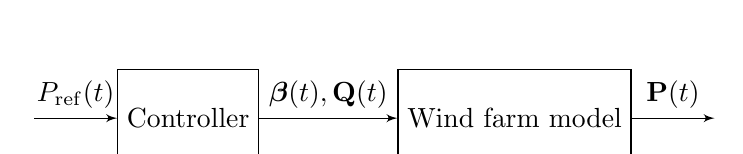
\begin{tikzpicture}[auto, node distance=2.25cm,>=latex']
% Blocks
\node [block, name=model] {Controller};
\node [io, left=3em of model.west] (reference){};
\node [block, right=5em of model] (farm) {Wind farm model};
\node [io, right=3em of farm.east] (Pfarm) {};
 
% Top input to output
\draw [->] (reference) -- node {$P_{\mathrm{ref}}(t)$} (model.west) {};
\draw [->] (model.east) -- node {$\boldsymbol \beta(t), \mathbf{Q}(t)$} (farm.west) {};
\draw [->] (farm.east) -- node {$\mathbf{P}(t)$} (Pfarm) {};
\end{tikzpicture}
\end{center}
\vspace{-0.5em}
\caption{\label{fig:block_diagram}Controlled wind farm system block diagram showing the model-based receding horizon controller and model wind farm. $P_\text{ref}(t)$ is the power reference signal, $\boldsymbol \beta(t)$ is the vector of pitch angles, $\mathbf{Q}(t)$ is the vector of generator torque, and $\mathbf{P}(t)$ is the vector of measured power generation.}
\end{figure}

All controlled cases are compared to the behavior of a wind farm operating under the traditional maximum power point control paradigm; i.e. each turbine operates at its maximum power point in region 2. In this regime, the blade pitch angle is kept fixed at the optimal value $\beta = \beta_*$ and the generator torque $Q = K\omega^2$ has a gain $K = \frac{1}{2}\rho \pi \left(\frac{D}{2}\right)^5 \frac{C_{P*}}{\lambda_*^3}$~\cite{Pao2011a} that drives the tip speed ratio to the optimal power coefficient \mbox{$C_{P*} = C_P(\lambda_*, \beta_*)$}. Since each turbine operates to maximize its own power production, rather than farm-level power, this operating condition is sometimes referred to as ``greedy" control~\cite{Munters2017a}.

The reference signal is composed of a fixed power generation level $P_0$, which would typically be sold in the bulk power market, and a power regulation reserve $\Delta P$ that can be provided in the regulation market. The resulting signal is
\begin{equation}
P_\text{ref}(t) = P_0 + \Delta P \, r(t),
\end{equation} 
where the regulation signal \mbox{$-1 \le r(t) \le 1$} is used by the grid operator to modulate the regulation power delivered by the farm. We select a bulk power supply of \mbox{$P_0 =  0.85P_*$}, where $P_*$ is the ``greedy" pre-control generation, and a regulation supply of $\Delta P = 0.3P_*$. This corresponds to a derate (power setpoint reduction) of only 50\% of $\Delta P$. We use a synthetic regulation signal $r(t)$, shown in red in Figure~\ref{fig:Pref}, that declines to $r(t)=0$ for the first 10 minutes before requesting an up-regulation of $r(t) = 1$ between 10:00 min and 15:00 min. The up-regulation ramp is $\Delta P = 0.3P_*$ and lasts for 5 minutes, which is approximately the travel time of the wind through the entire farm.

\begin{figure}[thpb]
\begin{center}
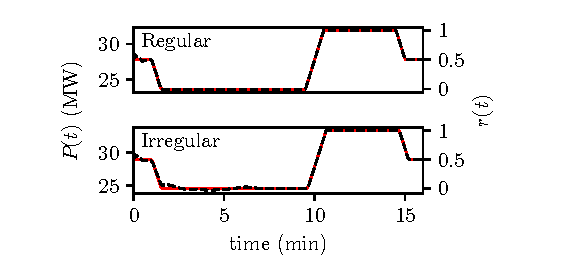
\includegraphics[width=0.75\textwidth]{./fig/Pref.pdf}
\vspace{-3em}
\end{center}
\caption{\label{fig:Pref}Total wind farm power output of both regular and regular layouts \mbox{$P(t) = \sum_{n=1}^N P_n(t)$} (\broken) compared to reference signal $P_\text{ref}(t)$ ({\color{red}\full}). The regulation signal $r(t)$ is also shown on the right side ordinate.}
\end{figure}

\begin{figure}[h]
\centering
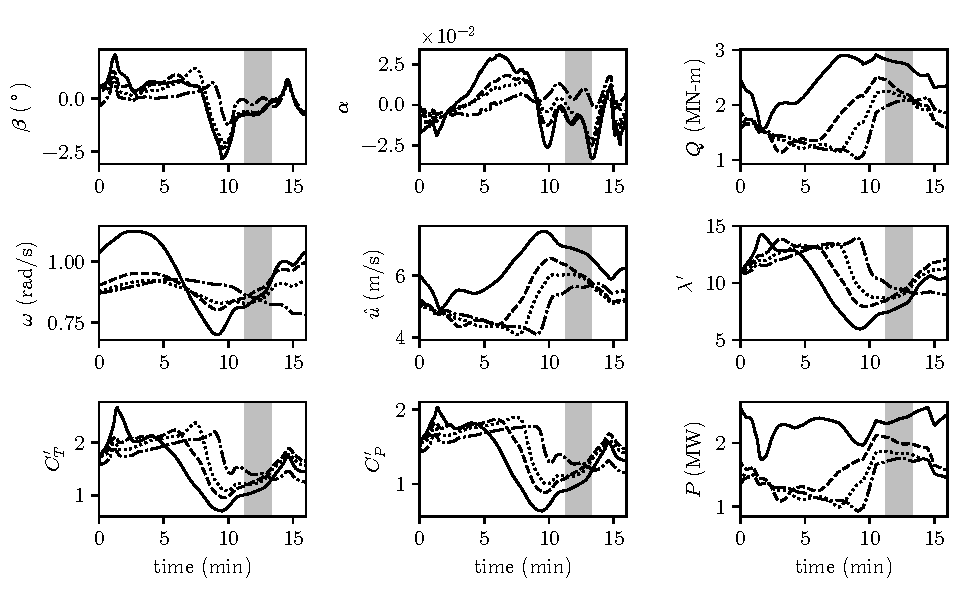
\includegraphics[width=\textwidth]{./fig/mpc.pdf}
\caption{Response of regular layout turbines 1 (\full), 2 (\broken), 3 (\dashed), and 4 (\dashdot) showing the pitch angle $\beta$, the auxiliary control variable $\alpha$, generator torque $Q$, rotor speed $\omega$, rotor-averaged velocity $\hat{u}$, local tip speed ratio $\lambda'$, local thrust coefficient $C_T'$, local power coefficient $C_P'$, and the generated power $P$. The up-regulation period $r(t) > 0.5$ is shaded gray between minutes 10 and 15.}
\label{fig:mpc}
\end{figure}

\begin{figure}[h]
\centering
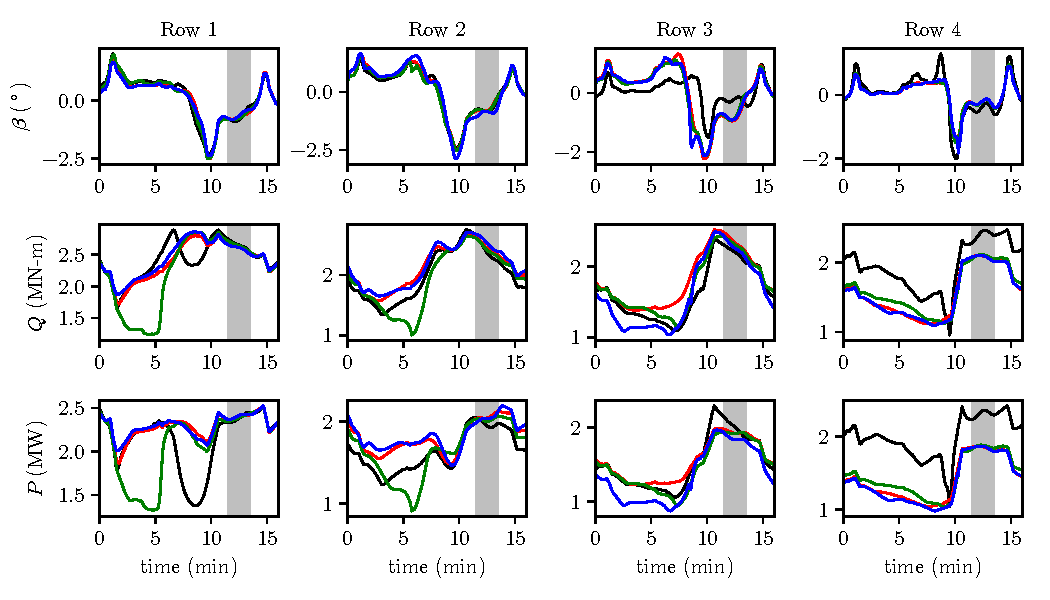
\includegraphics[width=\textwidth]{./fig/mpc2.pdf}
\caption{Response of all turbines in the irregular layout. The panels show the pitch angle $\beta$, generator torque $Q$, and generated power $P$. The up-regulation period $r(t) > 0.5$ is shaded gray between minutes 10 and 15. Colors denote turbines 1--4 (------), 5--8 ({\color{red}------}), 9--12 ({\color{blue}------}), 13--16 ({\color{forest_green}------}).}
\label{fig:mpc2}
\end{figure}


In both the regular and irregular layout, the controlled power output closely follows the power reference signal, as shown in Figure~\ref{fig:Pref}. The root mean square error
\begin{equation}
RMSE = \left(\frac{1}{T} \int\displaylimits_0^T \left[\sum_{n=1}^N Q_n(t) \omega_n(t) - P_\text{ref}(t)\right]^2 \, dt\right)^\frac{1}{2} \hspace{-1em}
\end{equation}
is 0.24\% and 0.56\% of $P_*$ for the regular and irregular configurations, respectively. This tracking performance is achieved with a signal that exceeds the ``greedy'' control power for a short period of time. This short-term over production is achieved by storing energy in the flow field and adjusting the rotational speed to hold kinetic energy in the rotors of the turbines, as described in more detail below.


\begin{figure}[thpb]
\centering
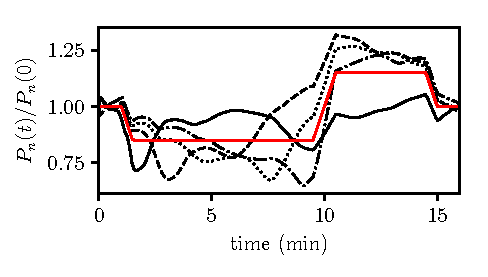
\includegraphics[width=0.5\textwidth]{./fig/Pnorm.pdf}
\vspace{-1.75em}
\caption{Power generation of regular layout turbines 1 (\full), 2 (\broken), 3 (\dashed), and 4 (\dashdot) normalized by their ``greedy" pre-control power generation compared to $P_\text{ref}(t)/P_*$ ({\color{red}\full}). Only one column is shown because all turbines in a row of the regular layout have the same control. Increased generation of turbines 2--4 for the 5-minute up-regulation period is enabled by storing energy in the flow field and rotation of the rotors.}
\label{fig:Pnorm}
\end{figure}

In the regularly arranged layout, the wakes do not expand enough to create spanwise interactions. As a result, the controller selects pitch and torque signals that are the same for all turbines in a particular row; i.e. the signals for turbines 1, 5, 9, and 13 are all the same. In a real wind farm, turbulent fluctuations in the wind field would break the equivalence of the control actions within a row. The power generation response of the controller for the turbines in the first column (turbines 1--4) is shown in Figure~\ref{fig:Pnorm}. The controller reduces the power generation of the first and last rows just preceding the up-regulation period, while keeping the generation of the second and third rows of turbines close to the pre-control power. The resulting generation during the up-regulation period is higher than the pre-control period for all downstream turbines, but this effect could not be sustained indefinitely. Since the first row of turbines cannot sustain generation higher than the optimal power point for five minutes, the first turbine produces near its pre-control output during the up-regulation period.

The pitch angle $\beta$, auxiliary control variable $\alpha$, generator torque $Q$, rotor speed $\omega$, rotor-averaged velocity $\hat{u}$, local tip speed ratio $\lambda'$, local thrust coefficient $C_T'$, local power coefficient $C_P'$, and the generated power $P$ trajectories for the first column of the regular layout are shown in Figure~\ref{fig:mpc}. The controller sequentially decreases the thrust and power coefficients of the upstream turbines, turbine 1 around $t = 5$:30 min, turbine 2 around $t = 7$:00 min, and turbine 3 around $t = 8$:30 min. These decreases in thrust coefficient reduce the magnitude of the wakes between the turbines, thus allowing higher velocity air to reach downstream turbines. The time of the decreases is closely tied to the advection time between turbines ($\approx 90$ s), allowing the velocity at each turbine to peak around 10:00 min, just prior to the up-regulation demand of the signal in Figure~\ref{fig:Pref}

The controller simultaneously uses pitch and generator torque to reduce the power production of the upstream turbines prior to the up-regulation period. All turbines pitch to feather between 8:00 min and 10:00 min, dropping the power and thrust coefficients. Furthermore, the generator torques are increased to slow down the rotor speed and reduce the tip speed ratio. On the other hand, the last turbine keeps its rotor speed slightly higher than the optimal tip speed ratio. This action stores kinetic energy that can later be extracted during the up-regulation period at 10:00 min.

The input and output trajectories for each turbine of the irregular layout are shown in Figure~\ref{fig:mpc2}. In this layout, each turbine has a different wake state and therefore the output power and control signals follow unique trajectories. However, the general trends of the regular configuration are also seen in these results. The thrust coefficients of upstream turbines decline prior to the up-regulation period via pitch-to-feather and increased generator torque actuation. Downstream turbines show a slight over-speeding of their rotors to store energy for the up-regulation period.

\section{Conclusions}
\label{sec:rhc2-conclusions}
A generalized dynamic wake model is presented that allows for irregular wind farm configurations, explicitly includes actuation of blade pitch angle and generator torque, and incorporates first-order drive train dynamics. These improvements are a significant step towards implementation of previously proposed model-based receding horizon control using existing wind turbine control loops. Control authority is improved by separately controlling each turbine and accounting for kinetic energy stored in the rotors.

Testing of the controller using wind farm plants consisting of the wake and turbine model and a synthetic power reference signal demonstrate the potential of this control design. Accounting for wake interactions and exploiting the storage of kinetic energy in the rotor, the controller is able to provide regulation power with derates less than the amount of regulation provided; i.e. $P_0 < P_* - \Delta P$. Further work includes adding a state and parameter estimation model~\cite{Shapiro2017b} as well as testing the closed-loop controller in high-fidelity wind farm simulations~\cite{Shapiro2018a} and operating wind farms. 
\chapter{Summary and future work}
\label{chap:conclusions}
\chaptermark{Summary and future work}

Grid frequency regulation will be an increasing challenge as wind energy and other renewable energy sources continue to grow. Developing controllers that allow wind farms to provide secondary frequency regulation for the grid effectively will therefore speed adoption of renewable energy sources in the future. This thesis works towards an integrated closed-loop model-based controller by deriving wake models for control applications, implementing sensing and estimation methods, and developing model-based receding horizon controllers.

While wake models have been extensively developing for decades, these models generally focused on maximizing power or minimizing loads in steady-state. In the context of frequency regulation, however, the dynamics of wind farm wake interactions become increasingly important, and a dynamic wake model is needed to develop control algorithms. As importantly, a control oriented dynamic wake model must be computationally efficient, solvable in fractions of a second. In Chapter~\ref{chap:dynwake} we develop a dynamic model of a wind farm wake from first principles. By making a few simplifying assumptions, such as linearized advection and time-invariance of the mixing rate of the wake with the surrounding air, the model reduces to a one-dimensional partial differential equation for the wake velocity deficit. In Section~\ref{sec:dynwake-1d} the model is further simplified by considering regular wind farm arrangements and using the Jensen model's square superposition approach. When compared to numerical simulations of a wind farm at start up, this simple dynamic wake model can predict the velocity at downstream wind turbines with enough accuracy to be included in a model-based control algorithm with closed-loop feedback.

Noticing the considerable disagreement of models of yawed turbines, a lifting line theory for the inviscid flow past a yawed wind turbine is developed in Chapter~\ref{chap:yaw}. Drawing on an analogy between a finite airfoil, the transverse lift distribution of a yawed actuator disk is shown to be elliptic. This elliptic distribution induces a constant transverse velocity behind the turbine, which can be combined with axial momentum conservation to derive expressions for the streamwise velocity deficit behind the turbine and the disk-averaged velocity through the rotor. When compared to simulations of yawed actuator disks, this lifting line theory more closely agrees than previous models. Finally, the lifting line theory is used as an initial condition for the wake model of Chapter~\ref{chap:dynwake}, matching measurements from the experiments of Bastankhah and Port\'{e}-Agel~\cite{Bastankhah2016a}. 

Although the dynamic model in Section~\ref{sec:dynwake-1d} provides acceptable agreement with numerical simulations, power measurements from wind farms can be used to improve the estimation capabilities of the model. The dynamic wake model, which is a nonlinear PDE, cannot be used directly in standard Kalman filter methods, however, because of the large state space and nonlinearity. Instead, we use an ensemble-based method that converges to the canonical Kalman filter and can be implemented in a computationally efficient way. Using an ensemble Kalman filter, we show in Chapter~\ref{chap:estimation} that power measurements can be used to improve estimates of the wake velocity deficit, wake expansion coefficients, and the inflow velocity. This approach is implemented in LES, providing good agreement with measured velocities and best-fit wake expansion coefficients.

In Chapter~\ref{chap:rhc} we build a model-based receding horizon controller around the wake model of Section~\ref{sec:dynwake-1d} and the state and parameter estimation of Chapter~\ref{chap:estimation}. This method is implemented using the PDE-constrained optimal control theories of Section~\ref{sec:methods-pdeopt}, and can therefore be applied in real time. Using LES as a ``virtual wind farm" we show that controlled wind farm can successfully track power reference signals and passes many of the qualification tests used by PJM. When compared against a static wake model-based controller, the dynamics of the wake model is shown to be important as the controlled wind farm of the static model cannot follow power reference signals. In Chapter~\ref{chap:rhc} we move toward pitch and generator torque based controls and demonstrate the potential improvements gained by this adaptation.

This study demonstrates that model-based receding horizon control can be used to effectively provide secondary frequency regulation services using wind farms. The results demonstrate that for the test system used (LES with the actuator disk turbine model) and the given initial conditions, up-regulation can be provided effectively with derates that are less than the maximum up-regulation requested. Previous studies~\cite{Aho2013a, Aho2014a, Jeong2014a} required a derate equal to the full magnitude of the largest increased power of the reference signal. The potential for reducing the required derate has important economic implications for wind farm operators. This derate reduction would mean that wind farms could generate more revenue from bulk power supply while still providing the same level of secondary frequency regulation. As a result, the cost-effectiveness of secondary regulation with wind farms could be altered significantly and wind farms may become a low-cost and dependable provider of secondary frequency regulation.

\section{Directions for future work}
While this thesis presents significant progress in allowing wind farms to provide secondary frequency regulation, more work is needed to fully implement the control approach presented in this thesis. The control algorithm presented in Chapter~\ref{chap:rhc2} needs to be tested in a high-fidelity simulation environment. Further tests in actuator line simulations or field tests would also be needed to fully vet the control algorithms. We also presented a yaw model that addresses limitations in the existing literature, but more work is needed implement and test the model in the context of wind farms with multiple turbines, implement sensing and estimation methods, and build a model-based controller for secondary frequency regulation. Finally, the approach of Chapter~\ref{chap:rhc} and~\ref{chap:rhc2} assumed that the regulation signal is known in advance instead of in real time. In order to implement the control in a realistic setting, forecasts of future regulation signals or control designs that maximize flexibility are needed.

Fortunately, the research presented in this thesis is part of a wide ranging effort from multiple research groups to advance wind energy integration into the power grid. No doubt significant advances will be made in the coming years. In the realm of yawed wind turbine research, researchers are rapidly understanding the wake behind a yawed turbine. Since initial observations of the curled wake several years ago~\cite{Howland2016a}, recent studies have shown the effect of wind shear, turbulence, and atmospheric stability on the evolution of the curled wake~\cite{Bartl2018a, Vollmer2016a}. The results of Chapter~\ref{chap:yaw} have already been used as an initial condition in an eddy-viscosity type model~\cite{Martinez2018a}. This rapid development will further our ability to model wind farms and improve control designs.

Recent work has also tried to address the down regulation strategy trade-offs alluded to in Chapter~\ref{chap:rhc2}. Specifically, what is the best downrate strategy to store kinetic energy in the rotor and reduce the thrust coefficient to maximize up-regulation potential? The approach of Chapter~\ref{chap:rhc2} attempts to computationally answer this equation, but other recent research~\cite{Hoek2018a, Kazda2018a, Siniscalchi-Minna2018a} is also trying to advance understanding by using power and thrust coefficient curves and quantifying power availability. In the coming years, a better understanding of the advantages of and potential trade-offs between storing energy in the rotation of the rotor and the flow field will improve control designs.

Since the beginning of this doctoral research, several new dynamic modeling and control approaches have been developed. PI control for secondary frequency regulation is still being studied and developed~\cite{vanWingerden2017a}. Dynamic yaw and thrust modulation has been used for power maximization~\cite{Munters2018a}. New controls-oriented models, such as 2D Navier-Stokes~\cite{Boersma2018a} and data-driven models~\cite{King2018a, Adcock2018a}, show promise. Low-resolution LES with adjoint-based estimation is an emerging research area~\cite{Bauweraerts2018a}. As these control methods mature and develop, a comprehensive comparison of their strengths and weaknesses will be needed to drive innovation.

The research presented in this thesis is ultimately part of a vibrant community of wind energy researchers trying to push our understanding of wind farm aerodynamics and improve control algorithms. As this research continues, our ability to increase the penetration of wind energy on the electric power system will continue to expand. With continued work, we can help meet the world's commitment to renewable energy and start to address the enormous challenges posed by global climate change.








% Appendix
\appendix
\chapter{Energy storage potential and efficiency}
\label{app}
\chaptermark{Energy storage potential and efficiency}

\section*{Energy storage}

We have presented a controller that can leverage energy stored in the rotation of the wind turbine rotors as well as the wind flow field. To get a sense of the relative energy storage capacity of these two mechanisms, the energy stored in the rotation of one turbine operating at the maximum power point is compared to the additional energy available in the flow field to a downstream turbine if the turbine is turned off. At the maximum power point, with optimal tip speed ratio $\lambda_* = \omega R / U_\infty$, the energy stored in the rotation of the rotor is
\begin{equation}
E_\text{rot} = \frac{1}{2} J \omega^2 =  \frac{1}{2} J \left( \frac{\lambda_* U_\infty}{R} \right)^2 ,
\end{equation}
where $J$ is the moment of inertia of the turbine rotor, $\omega$ is the rotational speed of the rotor, $U_\infty$ is the inflow velocity, and $R$ is the radius of the rotor swept area. For a turbine turned off, the energy stored in the wind flow field is equal to the additional power that can be generated by the downstream turbine $P_\text{add}$ times the advective time between the turbines $t_\text{adv}$
\begin{equation}
E_\text{wake} = P_\text{add} \, t_\text{adv}.
\end{equation}
Using the Jensen model~\cite{Jensen1983a}, the additional power is
\begin{equation}
P_\text{add} = \frac{1}{2} \rho \pi R^2 C_P \left[ U_\infty^3 - \left(U_\infty - \frac{2U_\infty a}{(1 + 2ks_x)^2}\right)^3 \right]
\end{equation}
where $C_P$ is the power coefficient, $a$ is the induction factor, $k$ is the wake expansion coefficient, and $2s_xR$ is the spacing between the turbines. The advective time is
\begin{equation}
t_\text{adv} = \frac{2 s_x R}{U_\infty}.
\end{equation}

The ratio of the energy stored in the flow field to the stored rotational energy is therefore
\begin{equation}
\frac{E_\text{wake}}{E_\text{rot}} = \frac{2 \rho \pi R^5s _x}{J} \frac{C_P}{\lambda_*^2} \left[ 1 - \left(1 - \frac{2 a}{(1 + 2ks_x)^2}\right)^3\right]
\end{equation}
If we consider a NREL 5MW turbine~\cite{Jonkman2009a}, with $U_\infty = 8$ m/s, $J = 4.0469\times 10^7$ kg m$^2$, $\lambda_* = 7.75$, $a = 0.292$, $C_P = 0.529$, $R = 63$ m, $\rho = 1.225$ kg/m$^3$, $k = 0.05$, and a streamwise spacing of $s_x = 7$, the rotational energy stored is $E_\text{rot} = 19.6$ MJ (5.5 kWh) and energy stored in the flow field is $E_\text{wake} = 112.2$ MJ (31.1 kWh). The corresponding ratio is
\begin{equation}
\left(\frac{E_\text{wake}}{E_\text{rot}}\right)_\text{NREL} = 5.725,
\end{equation}
which means that in this case the energy that can be stored in the flow is 5--6 times larger than the energy that can be stored in the rotation of the rotor. However, the ratio will depend on the configuration of the farm and will change for larger farms with more wake interactions.

\section*{Storage efficiency}
We have demonstrated that a wind farm can store energy in the flow field by reducing the power generation of upstream turbines. This effectively trades generation between time periods. To estimate the round trip storage efficiency of the wind farm, we simulate the effect of dynamically turning the first row of turbines in the wind farm discussed in Chapter~\ref{subsec:methods-les-farm} on and off, as shown in Figure~\ref{fig:app-dyn}.

\begin{figure}[h!]
\centering
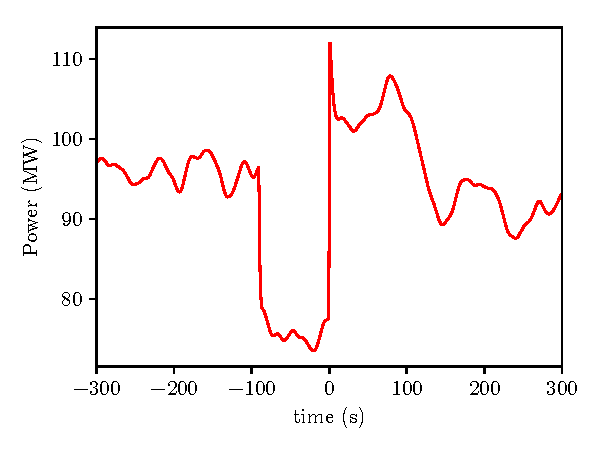
\includegraphics{./fig/fr.pdf}
\caption{Power generation of wind farm, where the first row of turbines is turned off at $t= -90$ s and turned back on at $t=0$ s. }
\label{fig:app-dyn}
\end{figure}

Initially, all turbines are operating at $C_T' = 4/3$, generating approximately 96 MW. At $t=-90$ s, the first row of turbines are turned off, $C_T' = 0$, reducing the generation to approximately 76 MW and eliminating the wake behind the first row of turbines. After 90 seconds, which is the advective time between the turbine rows, the wake from the first row is no longer affecting the generation of the second row. At this point, the first row of turbines is turned back on, which increases the generation to approximately 104 MW. This increased generation continues until around $t = 90$~s, at which point the generation returns to approximately 96 MW. This experiment demonstrates that time-shifting through energy storage in the flow field is feasible. In this case, the storage efficiency was around 45\%; however, the actual efficiency will depend on the turbulent inflow, layout of the farm control actions, and atmospheric conditions.



% References
\bibliographystyle{IEEEtran}
\bibliography{\string~/Dropbox/References/biblio}

% Vita
\begin{vita}
Carl Robert Shapiro was born in Atlanta, Georgia in 1987 and graduated from North Springs High School in Sandy Springs, Georgia in 2006. He received a B.S. in Engineering from Swarthmore College where he also minored in Music. Before beginning his graduate studies at Johns Hopkins, Carl worked as intern at National Renewable Energy Laboratory and an engineer at Steven Winter Associates. Carl received his M.S.E from Johns Hopkins University in 2016.
\end{vita}

\end{document}
